% ==== Document Class & Packages =====
\documentclass[12pt,hidelinks]{article}
	\usepackage[explicit]{titlesec}
	\usepackage{titletoc}
	\usepackage{tocloft}
	\usepackage{charter}
	\usepackage[many]{tcolorbox}
	\usepackage{amsmath}
	\usepackage{graphicx}
	\usepackage{xcolor}
	\usepackage{tikz,lipsum,lmodern}
	\usetikzlibrary{calc}
	\usepackage[english]{babel}
	\usepackage[utf8]{inputenc}
	\usepackage{fancyhdr}
	\usepackage{mathrsfs}
	\usepackage{empheq}
	\usepackage{fourier}% change to lmodern if fourier is no available
	\usepackage{wrapfig}
	\usepackage{fancyref}
	\usepackage{hyperref}
	\usepackage{cleveref}
	\usepackage{listings}
	\usepackage{varwidth}
	\usepackage{longfbox}
	\usepackage{geometry}
	\usepackage{marginnote}
	\usepackage{setspace}
	%\usepackage{subfigure}
	\usepackage{minted}
	\tcbuselibrary{theorems}
	\tcbuselibrary{breakable, skins}
	\tcbuselibrary{listings, documentation}
	\geometry{
		a4paper,
		left=33mm,
		right=33mm,
		top=20mm}
% ========= Path to images ============
%   - Direct the computer on the path 
% 	  to the folder containg the images
% =====================================
\graphicspath{{./images/}}
% ============= Macros ================
\newcommand{\fillin}{\underline{\hspace{.75in}}{\;}}
\newcommand{\solution}{\textcolor{mordantred19}{Solution:}}
\setlength{\parindent}{0pt}
\addto{\captionsenglish}{\renewcommand*{\contentsname}{Table of Contents}}
\linespread{1.2}
% ======== Footers & Headers ==========
\cfoot{\thepage}
\chead{}\rhead{}\lhead{}
% =====================================
\renewcommand{\thesection}{\arabic{section}}
\newcommand\sectionnumfont{% font specification for the number
	\fontsize{380}{130}\color{myblueii}\selectfont}
\newcommand\sectionnamefont{% font specification for the name "PART"
	\normalfont\color{white}\scshape\small\bfseries }
% ============= Colors ================
% ----- Red -----
\definecolor{mordantred19}{rgb}{0.68, 0.05, 0.0}
% ----- Blue -----
\definecolor{st.patrick\'sblue}{rgb}{0.14, 0.16, 0.48}
\definecolor{teal}{rgb}{0.0, 0.5, 0.5}
\definecolor{beaublue}{rgb}{0.74, 0.83, 0.9}
\definecolor{mybluei}{RGB}{0,173,239}
\definecolor{myblueii}{RGB}{63,200,244}
\definecolor{myblueiii}{RGB}{199,234,253}
% ---- Yellow ----
\definecolor{blond}{rgb}{0.98, 0.94, 0.75}
\definecolor{cream}{rgb}{1.0, 0.99, 0.82}
% ----- Green ------
\definecolor{emerald}{rgb}{0.31, 0.78, 0.47}
\definecolor{darkspringgreen}{rgb}{0.09, 0.45, 0.27}
\definecolor{applegreen}{rgb}{0.55, 0.71, 0.0}
% ---- White -----
\definecolor{ghostwhite}{rgb}{0.97, 0.97, 1.0}
\definecolor{splashedwhite}{rgb}{1.0, 0.99, 1.0}
% ---- Grey -----
\definecolor{whitesmoke}{rgb}{0.96, 0.96, 0.96}
\definecolor{lightgray}{rgb}{0.92, 0.92, 0.92}
\definecolor{floralwhite}{rgb}{1.0, 0.98, 0.94}
% ========= Part Format ==========
\titleformat{\section}
{\normalfont\huge\filleft}
{}
{20pt}
{\begin{tikzpicture}[remember picture,overlay]
	\fill[myblueiii] 
	(current page.north west) rectangle ([yshift=-13cm]current page.north east);   
\node[
	fill=mybluei,
	text width=2\paperwidth,
	rounded corners=6cm,
	text depth=18cm,
	anchor=center,
	inner sep=0pt] at (current page.north east) (parttop)
	{\thepart};%
\node[
	anchor=south east,
	inner sep=0pt,
	outer sep=0pt] (partnum) at ([xshift=-20pt]parttop.south) 
	{\sectionnumfont\thesection};
\node[
	anchor=south,
	inner sep=0pt] (partname) at ([yshift=2pt]partnum.south)   
	{\sectionnamefont SECTION};
\node[
	anchor=north east,
	align=right,
	inner xsep=0pt] at ([yshift=-0.5cm]partname.east|-partnum.south) 
	{\parbox{.7\textwidth}{\raggedleft#1}};
\end{tikzpicture}%
}
% ========= Hyper Ref ===========
\hypersetup{
	colorlinks,
	linkcolor={red!50!black},
	citecolor={blue!50!black},
	urlcolor={blue!80!black}
}
% ========= Example Boxes =============
\tcbset{
	defstyle/.style={
		fonttitle=\bfseries\upshape, 
		fontupper=\slshape,
		arc=0mm, 
		beamer,
		colback=blue!5!white,
		colframe=blue!75!black},
	theostyle/.style={
		fonttitle=\bfseries\upshape, 
		fontupper=\slshape,
		colback=red!10!white,
		colframe=red!75!black},
	visualstyle/.style={
		height=6.5cm,
		breakable,
		enhanced,
		leftrule=0pt,
		rightrule=0pt,
		bottomrule=0pt,
		outer arc=0pt,
		arc=0pt,
		colframe=mordantred19,
		colback=lightgray,
		attach boxed title to top left,
		boxed title style={
			colback=mordantred19,
			outer arc=0pt,
			arc=0pt,
			top=3pt,
			bottom=3pt,
		},
		fonttitle=\sffamily,},
	discussionstyle/.style={
		height=6.5cm,
		breakable,
		enhanced,
		rightrule=0pt,
		toprule=0pt,
		outer arc=0pt,
		arc=0pt,
		colframe=mordantred19,
		colback=lightgray,
		attach boxed title to top left,
		boxed title style={
			colback=mordantred19,
			outer arc=0pt,
			arc=0pt,
			top=3pt,
			bottom=3pt,
		},
		fonttitle=\sffamily},
	mystyle/.style={
		height=6.5cm,
		breakable,
		enhanced,
		rightrule=0pt,
		leftrule=0pt,
		bottomrule=0pt,
		outer arc=0pt,
		arc=0pt,
		colframe=mordantred19,
		colback=lightgray,
		attach boxed title to top left,
		boxed title style={
			colback=mordantred19,
			outer arc=0pt,
			arc=0pt,
			top=3pt,
			bottom=3pt,
		},
		fonttitle=\sffamily},
	aastyle/.style={
			height=3.5cm,
			enhanced,
			colframe=teal,
			colback=lightgray,
			colbacktitle=floralwhite,
			fonttitle=\bfseries,
			coltitle=black,
		attach boxed title to top center={
	  		yshift=-0.25mm-\tcboxedtitleheight/2,
	   		yshifttext=2mm-\tcboxedtitleheight/2}, 
		boxed title style={boxrule=0.5mm,
			frame code={ \path[tcb fill frame] ([xshift=-4mm]frame.west)
				-- (frame.north west) -- (frame.north east) -- ([xshift=4mm]frame.east)
				-- (frame.south east) -- (frame.south west) -- cycle; },
			interior code={ 
				\path[tcb fill interior] ([xshift=-2mm]interior.west)
				-- (interior.north west) -- (interior.north east)
				-- ([xshift=2mm]interior.east) -- (interior.south east) -- (interior.south west)
				-- cycle;} }
				},
	examstyle/.style={
		height=9.5cm,
		breakable,
		enhanced,
		rightrule=0pt,
		leftrule=0pt,
		bottomrule=0pt,
		outer arc=0pt,
		arc=0pt,
		colframe=mordantred19,
		colback=lightgray,
		attach boxed title to top left,
		boxed title style={
			colback=mordantred19,
			outer arc=0pt,
			arc=0pt,
			top=3pt,
			bottom=3pt,
		},
		fonttitle=\sffamily},
	doc head command={
		interior style={
			fill,
			left color=yellow!20!white, 
			right color=white}},
	doc head environment={
		boxsep=4pt,
		arc=2pt,
		colback=yellow!30!white,
		},
	doclang/environment content=text
}
% ============= Boxes ================
\newtcolorbox[auto counter,number within=section]{example}[1][]{
	mystyle,
	title=Example~\thetcbcounter,
	overlay unbroken and first={
		\path
		let
		\p1=(title.north east),
		\p2=(frame.north east)
		in
		node[anchor=
			west,
			font=\sffamily,
			color=st.patrick\'sblue,
			text width=\x2-\x1] 
		at (title.east) {#1};
	}
}
\newtcolorbox[auto counter,number within=section]{longexample}[1][]{
	examstyle,
	title=Example~\thetcbcounter,
	overlay unbroken and first={
		\path
		let
		\p1=(title.north east),
		\p2=(frame.north east)
		in
		node[anchor=
		west,
		font=\sffamily,
		color=st.patrick\'sblue,
		text width=\x2-\x1] 
		at (title.east) {#1};
	}
}
\newtcolorbox[auto counter,number within=section]{example2}[1][]{
	aastyle,
	title=Example~\thetcbcounter,{}
}
\newtcolorbox[auto counter,number within=section]{discussion}[1][]{
	discussionstyle,
	title=Discussion~\thetcbcounter,
	overlay unbroken and first={
		\path
		let
		\p1=(title.north east),
		\p2=(frame.north east)
		in
		node[anchor=
		west,
		font=\sffamily,
		color=st.patrick\'sblue,
		text width=\x2-\x1] 
		at (title.east) {#1};
	}
}
\newtcolorbox[auto counter,number within=section]{visualization}[1][]{
	visualstyle,
	title=Visualization~\thetcbcounter,
	overlay unbroken and first={
		\path
		let
		\p1=(title.north east),
		\p2=(frame.north east)
		in
		node[anchor=
		west,
		font=\sffamily,
		color=st.patrick\'sblue,
		text width=\x2-\x1] 
		at (title.east) {#1};
	}
}
% --------- Theorems ---------
\newtcbtheorem[number within=subsection,crefname={definition}{definitions}]%
	{Definition}{Definition}{defstyle}{def}%
\newtcbtheorem[use counter from=Definition,crefname={theorem}{theorems}]%
	{Theorem}{Theorem}{theostyle}{theo}
	%
\newtcbtheorem[use counter from=Definition]{theo}{Theorem}%
{
	theorem style=plain,
	enhanced,
	colframe=blue!50!black,
	colback=yellow!20!white,
	coltitle=red!50!black,
	fonttitle=\upshape\bfseries,
	fontupper=\itshape,
	drop fuzzy shadow=blue!50!black!50!white,
	boxrule=0.4pt}{theo}
\newtcbtheorem[use counter from=Definition]{DashedDefinition}{Definition}%
 {
 	enhanced,
 	frame empty,
 	interior empty,
 	colframe=darkspringgreen!50!white,
	coltitle=darkspringgreen!50!black,
	fonttitle=\bfseries,
	colbacktitle=darkspringgreen!15!white,
	borderline={0.5mm}{0mm}{darkspringgreen!15!white},
	borderline={0.5mm}{0mm}{darkspringgreen!50!white,dashed},
	attach boxed title to top center={yshift=-2mm},
	boxed title style={boxrule=0.4pt},
	varwidth boxed title}{theo}
%%%%%%%%%%%%%%%%%%%%%%%%%%%%%%%%%%%%%%%%
\newtcblisting[auto counter,number within=section]{disexam}{
	skin=bicolor,
	colback=white!30!beaublue,
	colbacklower=white,
	colframe=black,
	before skip=\medskipamount,
	after skip=\medskipamount,
	fontlower=\footnotesize,
	listing options={style=tcblatex,texcsstyle=*\color{red!70!black}},}
%%%%%%%%%%%%%%%%%%%%%%%%%%%%%%%%%%%%%%%

\begin{document}
\begin{titlepage}
	\centering % Center everything on the title page
	\scshape % Use small caps for all text on the title page
	\vspace*{1.5\baselineskip} % White space at the top of the page
% ===================
%	Title Section 	
% ===================

	\rule{13cm}{1.6pt}\vspace*{-\baselineskip}\vspace*{2pt} % Thick horizontal rule
	\rule{13cm}{0.4pt} % Thin horizontal rule
	
		\vspace{0.75\baselineskip} % Whitespace above the title
% ========== Title ===============	
	{	\Huge Dspace\\ 
			\vspace{4mm}
		MANUAL  \\	}
% ======================================
		\vspace{0.75\baselineskip} % Whitespace below the title
	\rule{13cm}{0.4pt}\vspace*{-\baselineskip}\vspace{3.2pt} % Thin horizontal rule
	\rule{13cm}{1.6pt} % Thick horizontal rule
	
		\vspace{1.75\baselineskip} % Whitespace after the title block
% =================
%	Information	
% =================
	{\large Leonard \\
		\vspace*{1.2\baselineskip}
	EMAIL: leonardcampelo@ibict.br} \\
	\vfill

\end{titlepage}
%%%%%%%%%%%%%%%%%%%%%%%%%%%%%%%%%%%%%%%%%%%%%%%%%%%%%%%%%%%
\tableofcontents
\vfill
\small{\noindent \textbf{About This File} \vspace{-3mm}\\
\noindent \rule{3.3cm}{0.5pt} \\
This file was created for the benefit of all teachers and students wanting to use Latex for tests/exams/lessons/thesis/articles etc.\\
The entirety of the contents within this file, and folder, are free for public use.}
\newpage
\newgeometry{
	left=29mm, 
	right=29mm, 
	top=20mm, 
	bottom=15mm}
%%%%%%%%%%%%%%%%%%%%%%%%%%%%%%%%%%%%%%%%%%%%%%%%%%%%%%%%%%%
\section{Introdução}
\newpage
    \subsection{O que é o DSpace?}
        Este manual oferece instruções sobre o uso do software DSpace. Além da instalação e configurações básicas.
        O DSpace é um dos softwares mais utilizados mundialmente para construção e gerenciamento de repositórios digitais e que apesar de ser uma ferramenta simples dispõe de muitos recursos.
        \singlespacing
        A utilização crescente do software para repositórios pelas instituições brasileiras e as constantes atualizações e mudanças ocorridas foram fatores que impulsionaram a criação deste manual. 
         \singlespacing
         Utilizando a versão 6.3 do DSpace, este documento foi estruturado contendo as principais funcionalidades necessárias para a gestão de um repositório digital, focando principalmente repositórios institucionais. Esclarece ainda sobre temas correlatos que podem auxiliar os gestores na qualidade de dados de seus repositórios como: as diretrizes de metadados e a ferramenta para correção de dado, OpenRefine.
        \singlespacing
        O manual está composto por seções explicando o funcionamento do DSpace, a estrutura em que as informações são organizadas, as principais ferramentas disponíveis para os administradores dos repositórios, como realizar o depósito de um documento, as tarefas que envolvem o fluxo de depósito, breves explicações sobre o formulário de entrada, informações sobre as principais diretrizes de metadados e esclarecimentos sobre o uso da ferramenta Google OpenRefine.
\newpage
        \singlespacing
\section{Como funciona o DSpace}
\newpage
    \subsection{Visão geral:}
        \singlespacing \textbullet \hspace{6pt} Crie as estruturas de armazenamento: comunidades, subcomunidades e coleções;
        
        \textbullet \hspace{6pt} Defina as políticas das comunidades, subcomunidades e coleções: como será o fluxo de depósito; quem poderá depositar em cada coleção; configurações de acesso – aberto, restrito ou embargado.

        \textbullet \hspace{6pt} Atribua permissões aos usuários do repositório: defina quem poderá fazer depósitos; quem poderá editar e excluir depósitos; quem fará a avaliação e revisão dos depósitos; quais serão os administradores;

        \subsection{Sobre as permissões}
        O gerenciamento do DSpace é realizado por meio de diferentes permissões de acesso. Isso significa que os usuários cadastrados no sistema podem ter funções diferentes e, por isso, têm acesso a diferentes funcionalidades e ferramentas do sistema. O usuário administrador é o único que pode realizar todas as ações no sistema, pode também delegar funções e permissões para outros usuários, inclusive dar permissões de administrador para outros usuários.
        
        \subsection{Sobre as políticas}
        É possível criar políticas para cada elemento integrante do repositório:
        
            \centerline{Comunidade}      
            \centerline{Subcomunidade}      
            \centerline{Coleção}      
            \centerline{Item}      
            \centerline{Bitstream}
        \singlespacing
        A política aplicada ao item será sempre aquela atribuída ao elemento de menor hierarquia. Por exemplo, uma determinada coleção possui uma política de tornar todos os seus itens disponíveis ao público geral (permissão READ ao grupo Anonymous). Contudo, um item pertencente a esta coleção pode ter uma política que restrinja o acesso a ele, mesmo que a coleção da qual faz parte (hierarquia superior) tenha uma política diferente. Da mesma forma, o item pode ser composto de vários arquivos (bitstreams) e restringir o acesso a apenas um ou alguns desses arquivos, já que é possível atribuir políticas específicas ao bitstream.
        \singlespacing
        \textbf{\underline{NOTA}}: \emph{Bitstreams}  são os arquivos de computadores comuns. Por exemplo, o arquivo PDF de uma tese é um \emph{bitstream} no contexto dos repositórios.
        \singlespacing
        \textbf{\underline{IMPORTANTE}}: se você alterar a política de uma coleção que já possui itens, a nova política só valerá para os itens depositados depois da mudança. Os itens existentes permanecerão com as políticas antigas, ou seja, não serão atualizados automaticamente. Para atualizá-los, siga os procedimentos descritos em 5.3.4 Ferramenta avançada de administração de políticas.
\newpage
        Visualização das comunidades e coleções:
        
        \begin{figure}[!htp]
                \centering
                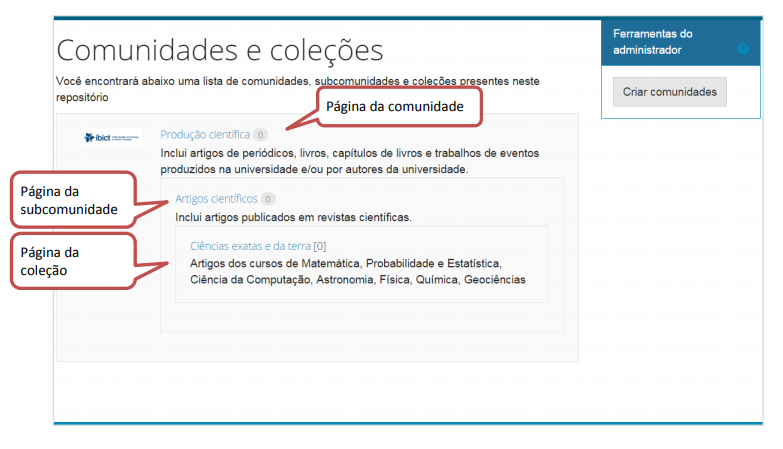
\includegraphics[scale=0.8]{figura/Figura1.png}
                \caption{Visualização das comunidades e coleções}
            \label{Rotulo}
        \end{figure}
        
\newpage
\section{Logar no repositório}
\newpage
    Para fazer o login no sistema é necessário ser um usuário registrado e ter uma senha de acesso. Para se registrar no sistema, siga os passos abaixo (1-6). Caso você já seja cadastrado no sistema pule para o passo 7
    \subsection{Registrar novo usuário no repositório}
    
    Passo 1: Na barra superior, clique no menu “Entrar em:” e acesse <Meu espaço>.
     \begin{figure}[!htp]
                \centering
                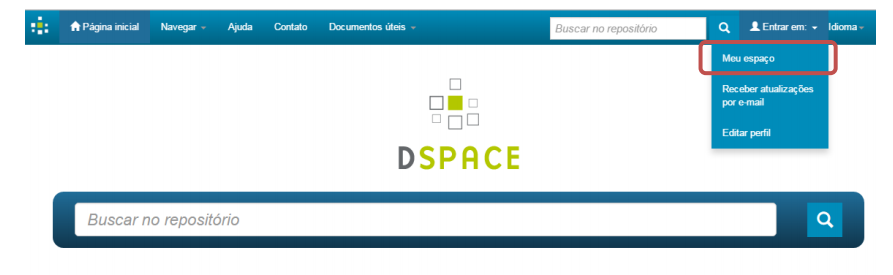
\includegraphics[scale=0.7]{figura/Figura2.png}
                \caption{Meu espaço}
            \label{Rotulo}
        \end{figure}   
        
       Passo 2 : Clique em <Usuário novo? Clique aqui para se registrar>. 
       
       \begin{figure}[!htp]
                \centering
                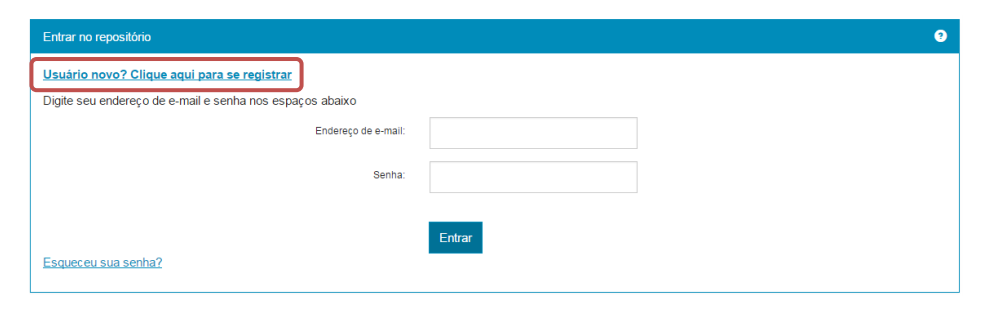
\includegraphics[scale=0.6]{figura/Figura3.png}
                \caption{Figura 3 - Cadastro de novo usuário}
            \label{Rotulo}
        \end{figure}  
        
    
        Passo 3: Informe seu endereço de e-mail que será cadastrado no sistema e clique em <Registrar>. Note que o endereço de e-mail cadastrado será utilizado para o envio de mensagens do sistema para você.
        
        \begin{figure}[!htp]
                \centering
                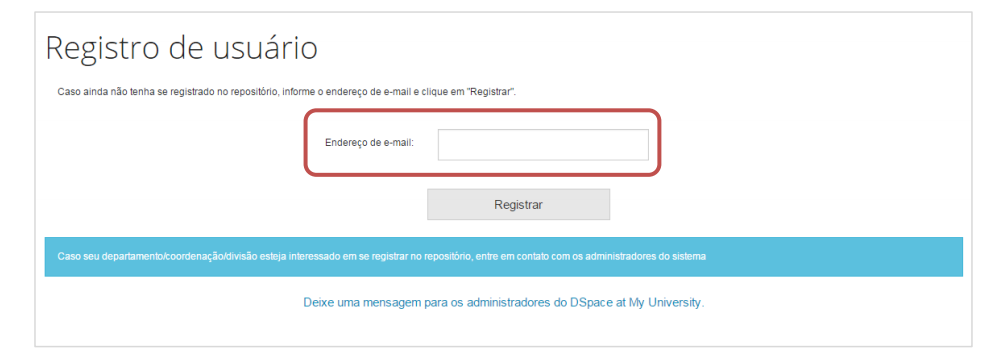
\includegraphics[scale=0.6]{figura/Figura4.png}
                \caption{Registro de usuário}
            \label{Rotulo}
        \end{figure}
\newpage        
        Passo 4: Após informar o endereço de e-mail e clicar em registrar, deverá aparecer uma mensagem informando que seu e-mail foi registrado e que você receberá uma mensagem no e-mail cadastrado. Caso isto não aconteça repita o passo três.
        
        \begin{figure}[!htp]
                \centering
                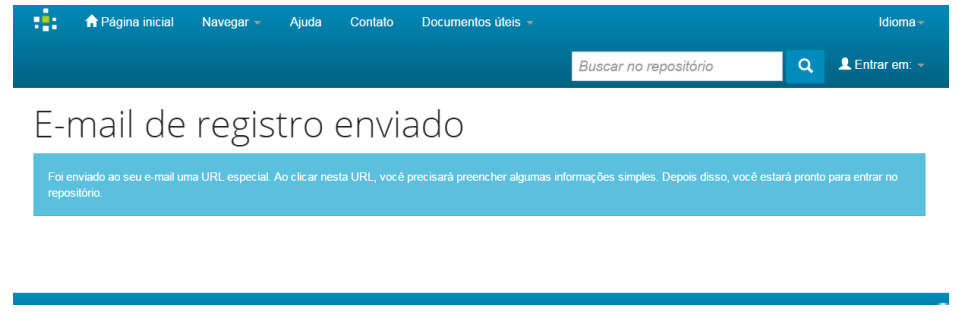
\includegraphics[scale=0.6]{figura/Figura5.png}
                \caption{Confirmação de registro}
            \label{Rotulo}
        \end{figure}
        
        Passo 5: Abra a mensagem que você recebeu na conta de e-mail registrada e clique no link que foi enviado.
        \singlespacing
        Passo 6: Ao clicar no link, uma nova página do repositório será aberta. Preencha as informações solicitadas e clique em <Complete o registro>. É obrigatório o preenchimento do “Primeiro nome” e do “Último nome”. 
        
        \begin{figure}[!htp]
                \centering
                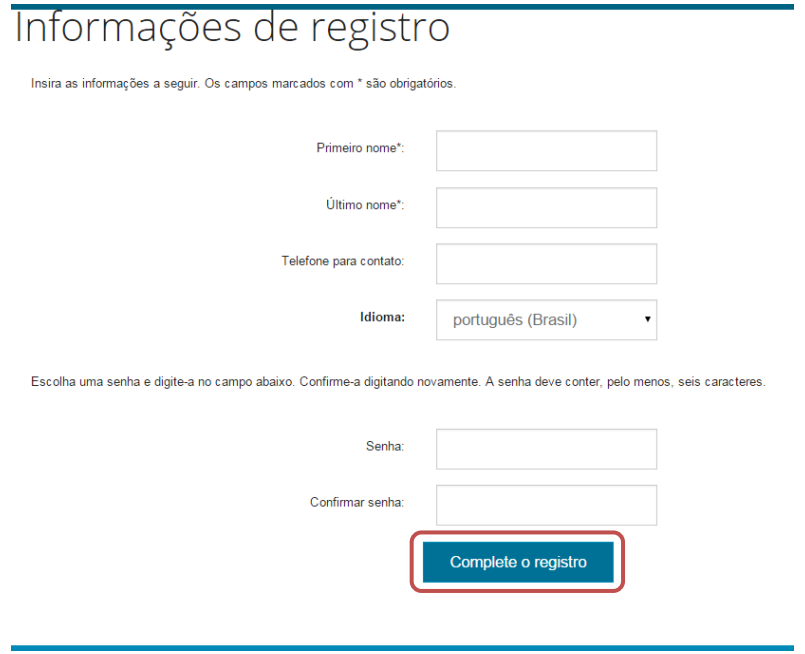
\includegraphics[scale=0.5]{figura/Figura6.png}
                \caption{Confirmação de registro}
            \label{Rotulo}
        \end{figure}
        
\newpage
        \subsection{Logar no repositório a partir de uma conta já existente}
        
        Passo 7: Na barra superior, clique no menu “Entrar em:” e acesse <Meu espaço>.
        
        \begin{figure}[!htp]
                \centering
                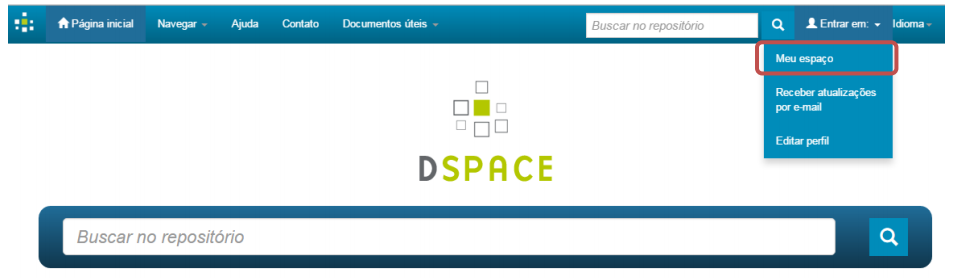
\includegraphics[scale=0.6]{figura/Figura7.png}
                \caption{Meu espaço}
            \label{Rotulo}
        \end{figure}
        
        Passo 8: Informe o endereço de e-mail cadastrado no repositório, a senha de acesso e clique em <Entrar>.
        
        \begin{figure}[!htp]
                \centering
                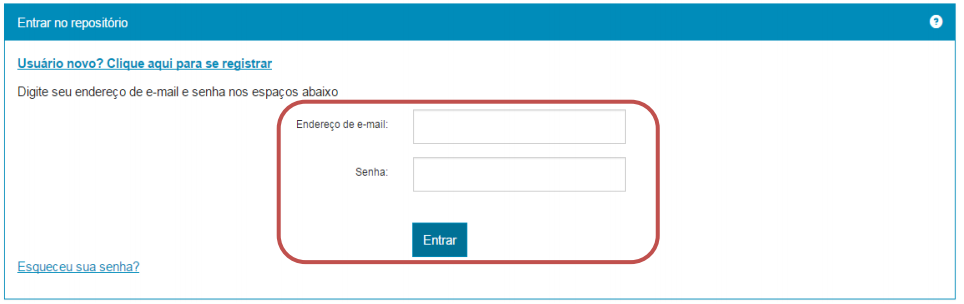
\includegraphics[scale=0.6]{figura/Figura8.png}
                \caption{Entrar no repositório}
            \label{Rotulo}
        \end{figure}
        
\newpage
        Passo 9: Acesso à “Meu espaço”. Após o login, você será direcionado a página <Meu espaço>, que apresenta as opções de iniciar um novo depósito, visualizar depósitos aceitos ou ver as tarefas pendentes:
        
        \begin{figure}[!htp]
                \centering
                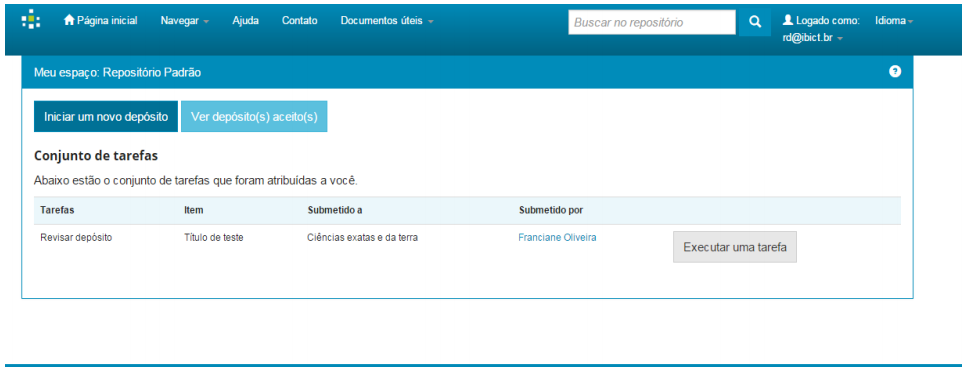
\includegraphics[scale=0.6]{figura/Figura9.png}
                \caption{Acesso à página “Meu espaço”}
            \label{Rotulo}
        \end{figure}
        
        
\newpage        
\section{Criar comunidades, subcomunidades e coleções}
\newpage

    Para iniciar o depósito de arquivos no repositório é recomendável que sejam criadas as
    estruturas de \underline{comunidades}, \underline{subcomunidades} e \underline{coleções}. 
    \singlespacing
    A criação destas três estruturas não é obrigatória. É possível criar uma única comunidade e depositar todos os arquivos na mesma comunidade. No entanto, a estrutura de comunidades, subcomunidades e coleções possui a funcionalidade de organizar o conteúdo dentro do repositório, permitindo assim melhor navegabilidade e atribuição de políticas e permissões diferenciadas segundo necessidades determinadas. Um exemplo de organização em comunidades, subcomunidades e coleções é apresentado a seguir:
    
    \begin{figure}[!htp]
                \centering
                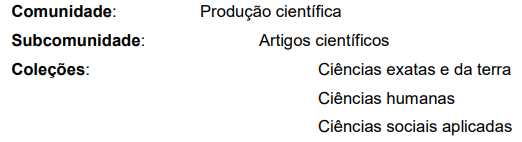
\includegraphics[scale=0.6]{figura/Comunidades.png}
            \label{Rotulo}
        \end{figure}
    
        \subsection{Criação de comunidade}
        
        Passo 1: Na barra superior, clique no menu “Navegar” e acesse <Comunidades e coleções>. 
        
        \begin{figure}[!htp]
                \centering
                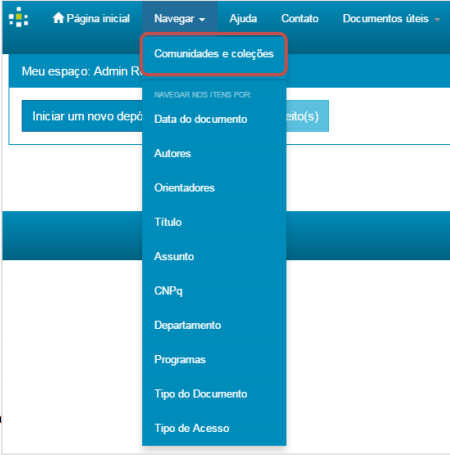
\includegraphics[scale=0.8]{figura/Figura10.png}
                \caption{Comunidades e coleções}
            \label{Rotulo}
        \end{figure}
    
\newpage
     Passo 2: Em ferramenta do administrador, clique em "Criar comunidades". 
     
     \begin{figure}[!htp]
                \centering
                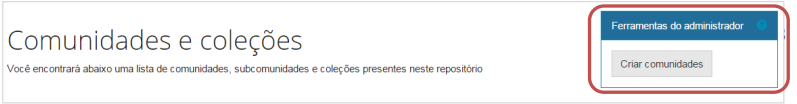
\includegraphics[scale=0.8]{figura/Figura11.png}
                \caption{Como criar comunidades}
            \label{Rotulo}
        \end{figure}
        
    Passo 3: Descreva a comunidade que será criada nos campos adequados e clique em <Criar>. Note que apenas o campo “Nome” é obrigatório, no entanto o preenchimento dos outros campos pode ser importante para prestar informações para os gestores que alimentarão a comunidade e para os usuários finais.
    
    \begin{figure}[!htp]
                \centering
                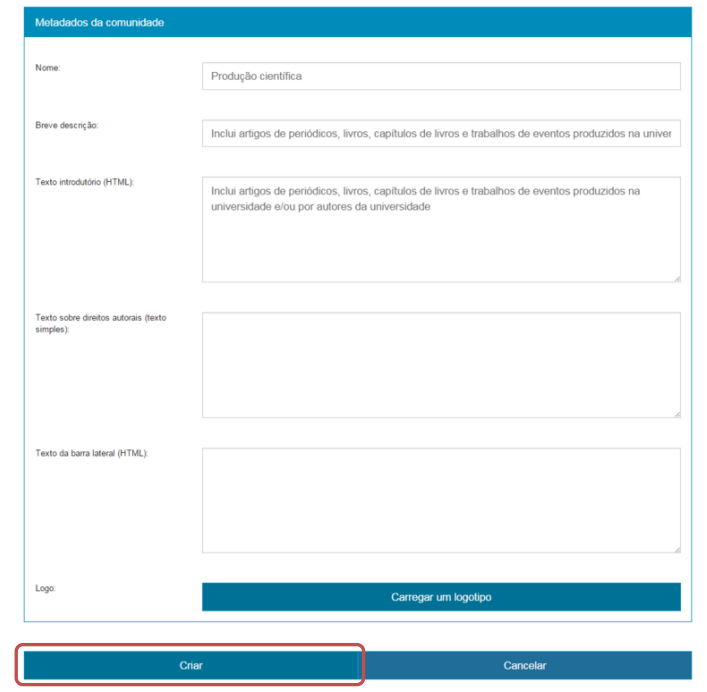
\includegraphics[scale=0.9]{figura/Figura12.png}
                \caption{Criar comunidade}
            \label{Rotulo}
        \end{figure}

\newpage
    Para saber mais sobre o preenchimento dos campos, siga as orientações abaixo:
    \singlespacing
    \textbullet \hspace{6pt} \textbf{Nome:} informe o nome que será dado à comunidade. Exemplo: Produção científica.
    \singlespacing
    \textbullet \hspace{6pt} \textbf{Texto introdutório (HTML):} insira um texto sobre a comunidade. Permite o uso de tags html que alteram a apresentação do texto. Exemplo: <p>Inclui artigos de periódicos, livros, capítulos de livros e trabalhos de eventos <b> produzidos na universidade </b> e/ou por autores da universidade.</p>
    \singlespacing
    \textbullet \hspace{6pt} \textbf{Texto sobre direitos autorais:} insira um texto sobre os direitos autorais que serão estabelecidos para os documentos da comunidade.
    \singlespacing
    \textbullet \hspace{6pt} \textbf{Texto da barra lateral:}  insira outro texto que queira para descrever a comunidade que aparecerá na barra lateral da página da comunidade.
    \singlespacing
    Passo 4: Atribuir um logotipo à comunidade. Ao criar uma comunidade é possível ainda relacioná-la ao seu logotipo, caso ela tenha uma imagem representativa. Para o uso do logo pela comunidade clique em <Carregar um logotipo>.
    
    \begin{figure}[!htp]
                \centering
                
\includegraphics[scale=0.8]{figura/Figura13.png}
                \caption{Carregar logotipo}
            \label{Rotulo}
        \end{figure}
        
    Passo 5: Clique em <Escolher arquivo> para selecionar uma imagem armazenada em seu computador. 
    
    \begin{figure}[!htp]
                \centering
                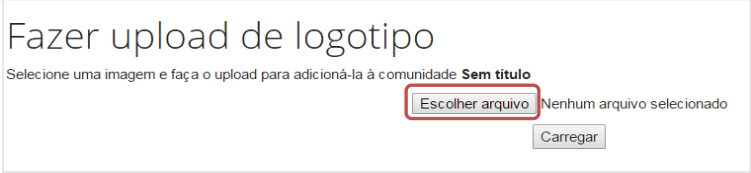
\includegraphics[scale=0.8]{figura/Figura14.png}
                \caption{Carregar logotipo}
            \label{Rotulo}
        \end{figure}
        
\newpage
    Passo 6: Selecione a imagem navegando pelas pastas de seu computador e clique em <Carregar>.
    
    \begin{figure}[!htp]
                \centering
                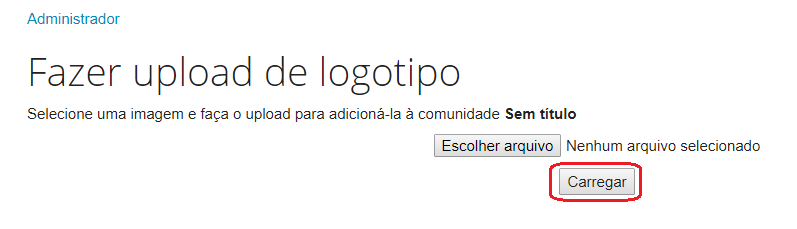
\includegraphics[scale=0.8]{figura/Figura15.png}
                \caption{Upload do arquivo}
            \label{Rotulo}
        \end{figure}
        
    Passo 7: Ao carregar o logotipo, a imagem poderá ser visualizada na página de gerenciamento da comunidade. Nela você poderá alterar a imagem carregada por outra, clicando em <Carregar novo logotipo> ou Excluir a imagem carregada, clicando em <Deletar (logotipo)>.
    
    \begin{figure}[!htp]
                \centering
                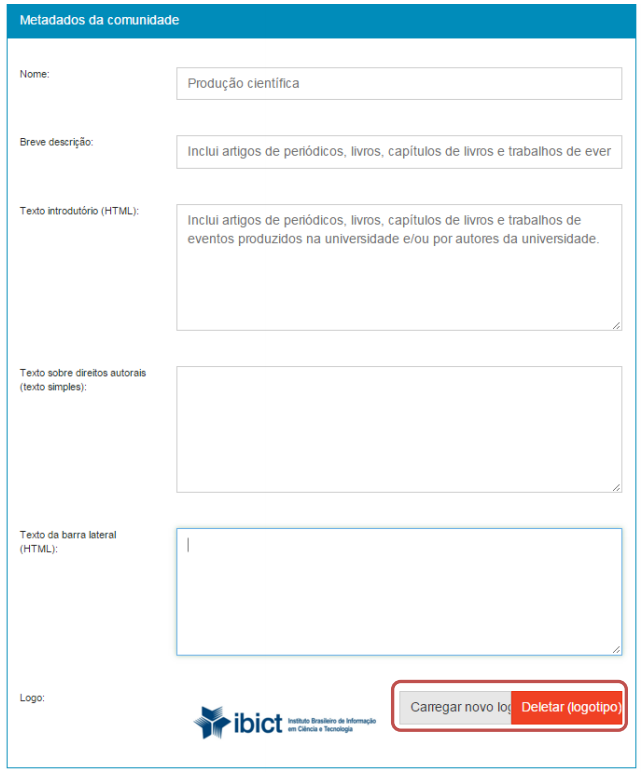
\includegraphics[scale=0.7]{figura/Figura16.png}
                \caption{Editar comunidade}
            \label{Rotulo}
        \end{figure}
        
    \subsection{Editar comunidade}
    
    Passo 1: Para editar alguma configuração da comunidade, entre na página da comunidade e clique em <Editar>.
    
    \begin{figure}[!htp]
                \centering
                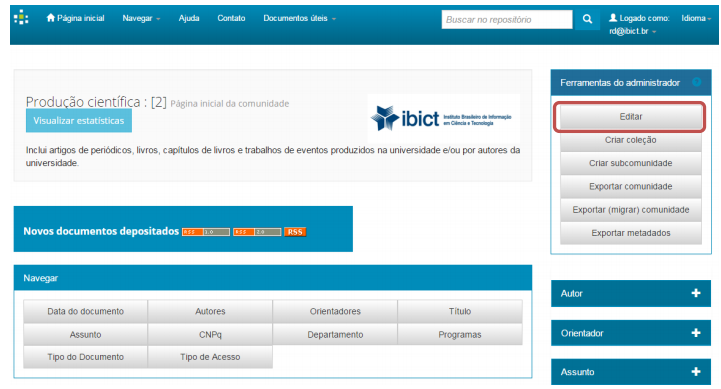
\includegraphics[scale=0.8]{figura/Figura17.png}
                \caption{Editar configuração da comunidade}
            \label{Rotulo}
        \end{figure}
        
    Passo 2: A página de edição assemelha-se com a imagem abaixo. Além de poder modificar a descrição da comunidade, você poderá:
    \singlespacing
    Excluir a comunidade, clicando em “Deletar esta comunidade”;
    Selecionar, mudar ou excluir os usuários administradores dessa comunidade;
    Estabelecer e editar políticas para a comunidade;
    Acessar as ferramentas de curadoria da comunidade.
    
    \begin{figure}[!htp]
                \centering
                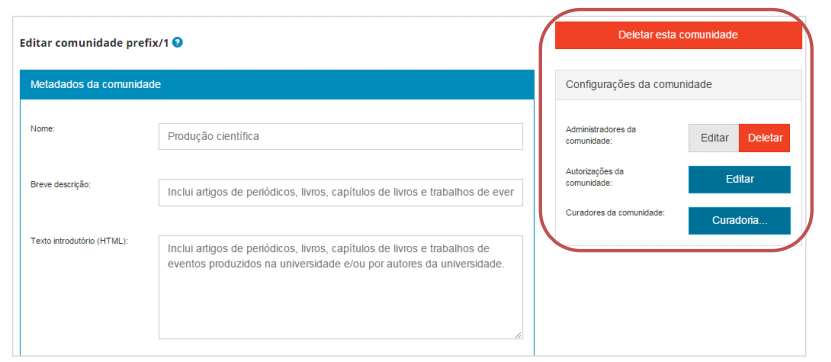
\includegraphics[scale=0.7]{figura/Figura18.png}
                \caption{Editar comunidade}
            \label{Rotulo}
        \end{figure}
        
\newpage
    \subsection{Estabelecimento de políticas para as comunidades}

    Para cada comunidade criada também é permitida a atribuição de grupos de usuários e políticas específicas para o seu gerenciamento.
    \singlespacing
    Passo 1: Acesse a página de edição da comunidade. Caminho:
    
    \begin{figure}[!htp]
                \centering
                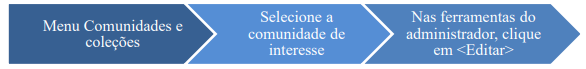
\includegraphics[scale=0.6]{figura/MenuComunidadesColecoes.png}
            \label{Rotulo}
        \end{figure}
    
    Passo 2: Clique em <Criar> para estabelecer um grupo de usuários como Administradores da comunidade.
    
    \begin{figure}[!htp]
                \centering
                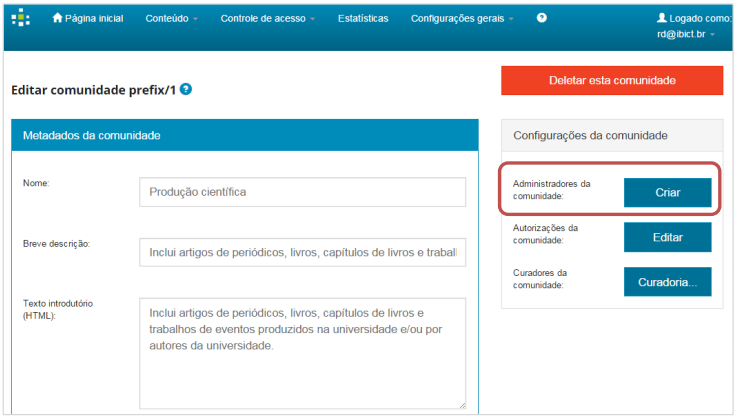
\includegraphics[scale=0.7]{figura/Figura19.png}
                \caption{Criar grupo de administradores da comunidade}
            \label{Rotulo}
        \end{figure}
    
    Passo 3: Para selecionar usuários específicos clique em <Selecionar usuários>.
    
    \begin{figure}[!htp]
                \centering
                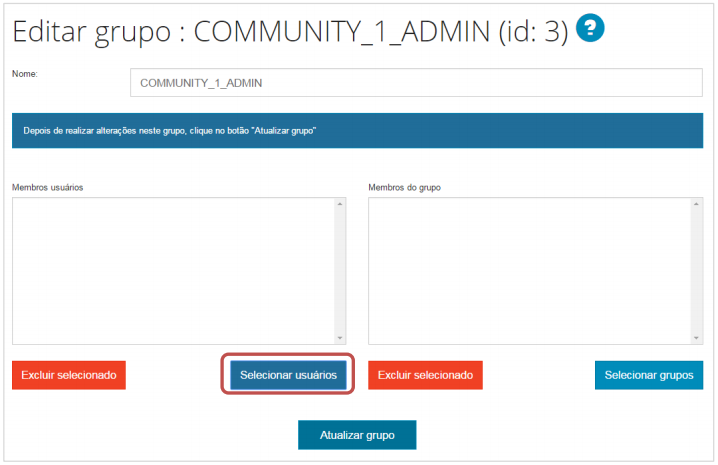
\includegraphics[scale=0.7]{figura/Figura20.png}
                \caption{Selecionar usuários}
            \label{Rotulo}
        \end{figure}
        
\newpage

    Passo 4: Uma lista com todos os usuários já cadastrados no repositório será aberta. Selecione os
    usuários que receberão as permissões de administrador da comunidade e clique em <Adicionar>
    
    \begin{figure}[!htp]
                \centering
                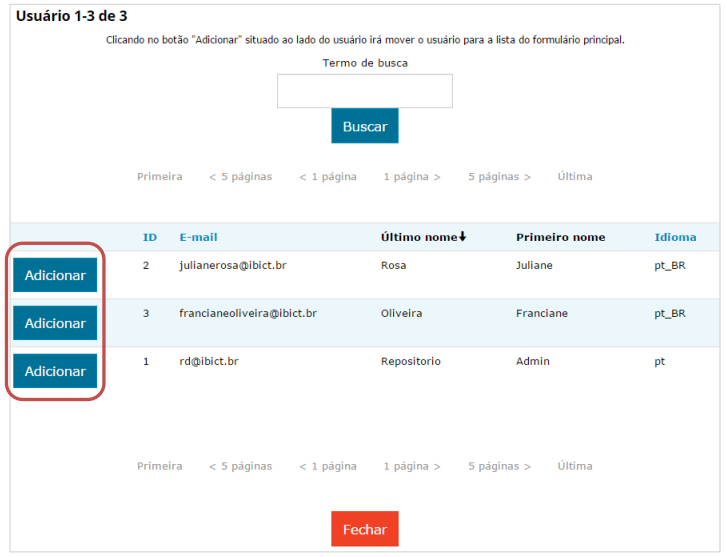
\includegraphics[scale=0.6]{figura/Figura21.png}
                \caption{Selecionar administradores}
            \label{Rotulo}
        \end{figure}
    
    \singlespacing
    Note que é possível navegar pela lista ou realizar uma busca pelo nome dos usuários cadastrados no campo “Termo de busca”.
    \singlespacing
    Passo 5: Após selecionados os usuários, estes deverão aparecer na caixa “Membros usuários”. Para finalizar esta ação clique em <Atualizar grupo>.
    \singlespacing
    \begin{figure}[!htp]
                \centering
                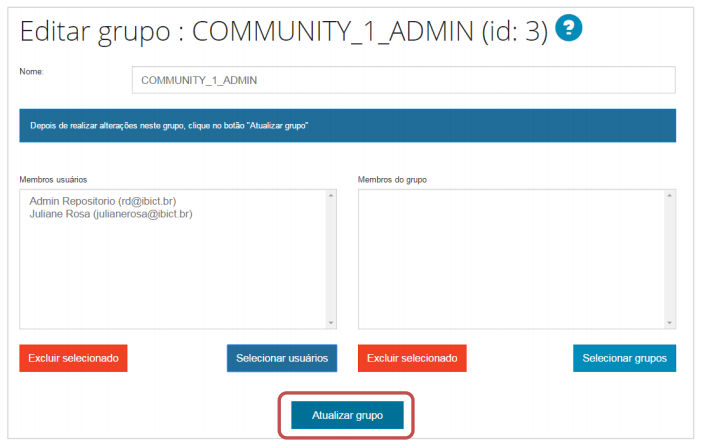
\includegraphics[scale=0.7]{figura/Figura22.png}
                \caption{Atualizar grupo}
            \label{Rotulo}
        \end{figure}

\newpage
    
    Passo 6: Caso queira retirar algum usuário da lista “Membros usuários” da comunidade, selecione o usuário e clique em <Excluir selecionado>.
    
    \begin{figure}[!htp]
                \centering
                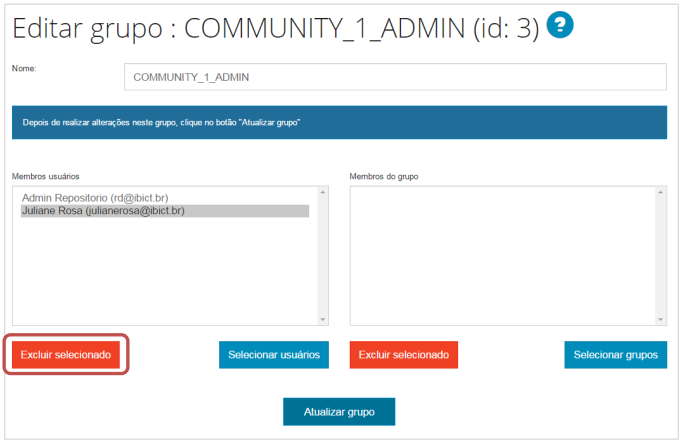
\includegraphics[scale=0.7]{figura/Figura23.png}
                \caption{Excluir membro do grupo}
            \label{Rotulo}
        \end{figure}
        
    Passo 7: O mesmo procedimento para a atribuição de usuários pode ser feito para grupo de usuários. Para tanto, clique em <Selecionar grupos>.
    
    \begin{figure}[!htp]
                \centering
                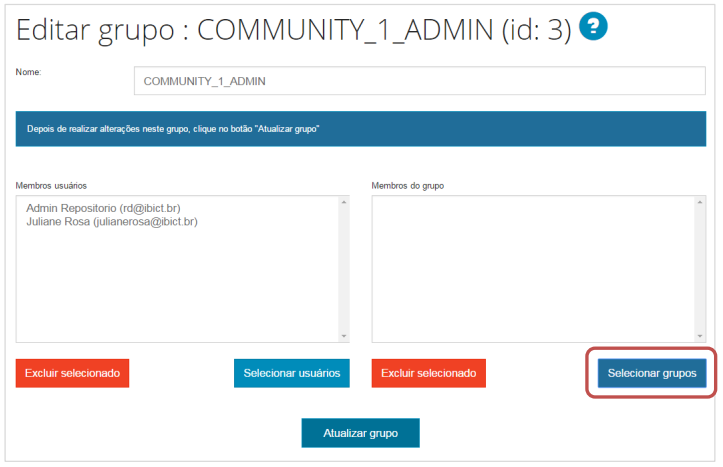
\includegraphics[scale=0.7]{figura/Figura24.png}
                \caption{Grupo de usuários}
            \label{Rotulo}
        \end{figure}

\newpage
    Passo 8: Uma lista com todos os grupos criados será aberta em uma nova janela. Selecione os grupos que receberão as permissões de administrador da comunidade e clique em <Adicionar>.
    
    \begin{figure}[!htp]
                \centering
                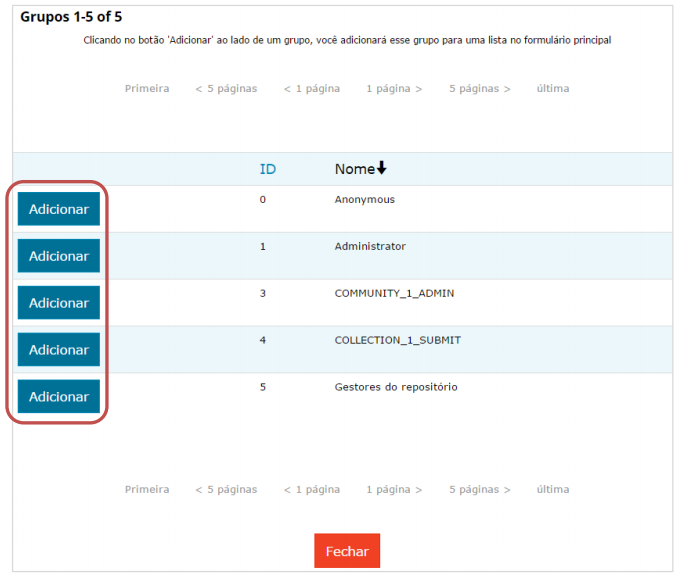
\includegraphics[scale=0.7]{figura/Figura25.png}
                \caption{Permissões aos grupos}
            \label{Rotulo}
        \end{figure}
    
    Passo 9: Depois de selecionado(s) o(s) grupo(s), este(s) deverão aparecer na caixa “Membros do grupo”. Para finalizar esta ação clique em <Atualizar grupo>.
    
    \begin{figure}[!htp]
                \centering
                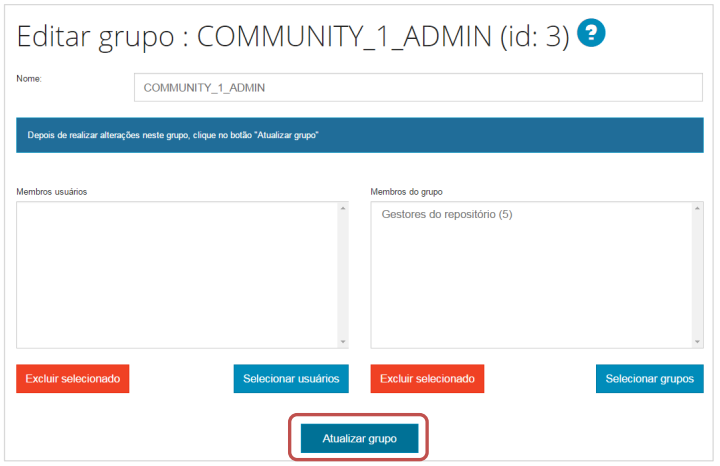
\includegraphics[scale=0.7]{figura/Figura26.png}
                \caption{Confirmar membros do grupo}
            \label{Rotulo}
        \end{figure}
        
\newpage
    Passo 10: Caso queira retirar algum grupo da lista “Membros do grupo” da comunidade, selecione o grupo e clique em <Excluir selecionado>.
    
    \begin{figure}[!htp]
                \centering
                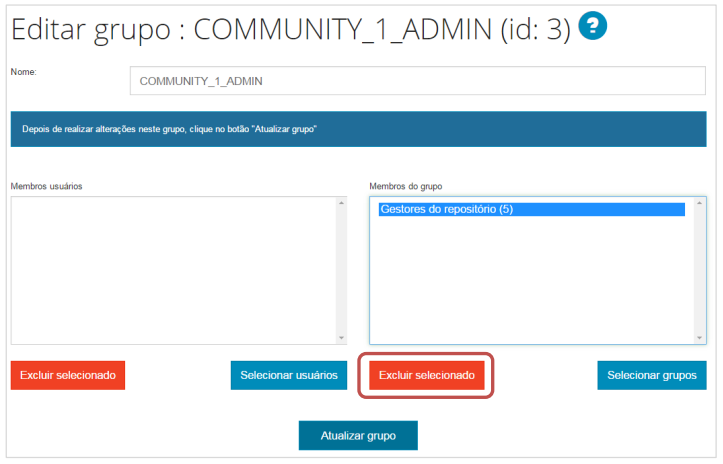
\includegraphics[scale=0.7]{figura/Figura27.png}
                \caption{Excluir membros do grupo}
            \label{Rotulo}
        \end{figure}
        
    Passo 11: Concluída esta etapa, volte para a comunidade para estabelecer suas políticas de funcionamento. Dentro da página <Editar comunidade>, o estabelecimento de políticas de funcionamento será feito na seção “Autorizações da comunidade”, clicando em <Editar>
    
    \begin{figure}[!htp]
                \centering
                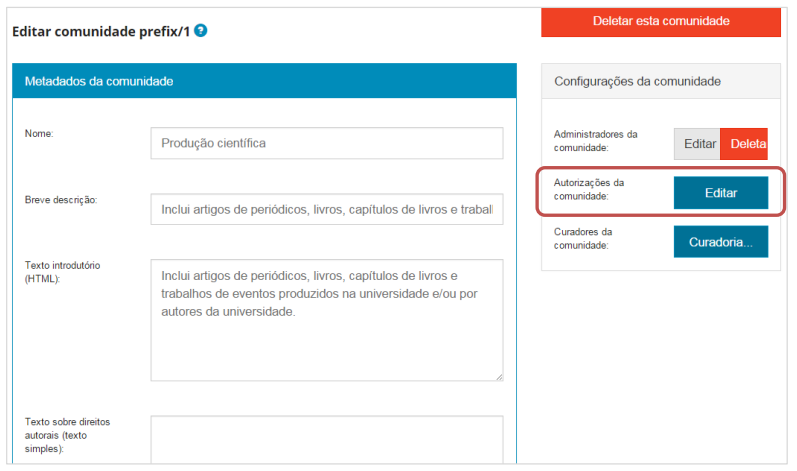
\includegraphics[scale=0.7]{figura/Figura28.png}
                \caption{Estabelecer políticas de funcionamento da comunidade}
            \label{Rotulo}
        \end{figure}
        
\newpage
        
    Passo 12: Para estabelecer uma política diferente da criada automaticamente para a coleção clique em <Adicionar nova política>.
    \singlespacing
    A política criada automaticamente para todas as coleções consiste em permissões de administração do sistema para os usuários pertencentes ao grupo administrador e permissões de navegação e leitura dos documentos depositados na coleção por todos os usuários (Anonymous), exceto dos itens embargados e restritos.
    
    \begin{figure}[!htp]
                \centering
                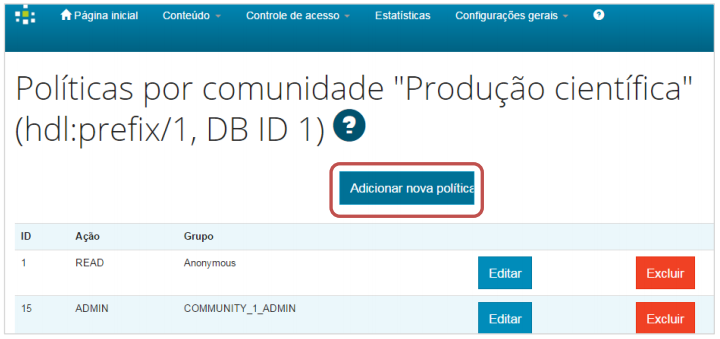
\includegraphics[scale=0.8]{figura/Figura29.png}
                \caption{Estabelecer políticas de funcionamento da comunidade}
            \label{Rotulo}
        \end{figure}
    
    Passo 13: Selecione o grupo de usuários, a permissão que lhe será dada e clique em <Salvar>.
    
    \begin{figure}[!htp]
                \centering
                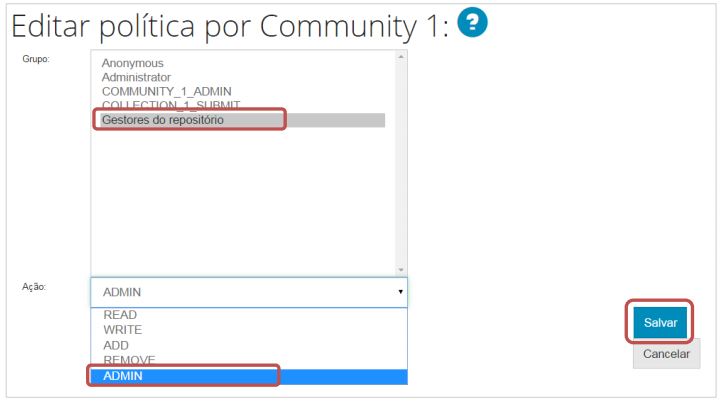
\includegraphics[scale=0.8]{figura/Figura30.png}
                \caption{Editar política por comunidade}
            \label{Rotulo}
        \end{figure}

\newpage
    Informações sobre as permissões:\\
    READ – permissão de visualização/leitura dos registros; \\
    WRITE – permissão de edição dos itens da comunidade;
    ADD – permissão para adicionar/depositar itens dentro da comunidade;
    REMOVE – permissão para remover/excluir itens da comunidade;
    ADMIN – permissão de administrador da comunidade (possui todas as permissões).
    
  \subsection{Criação de subcomunidade}  
  
  Passo 1: Para criar uma subcomunidade, entre em uma comunidade e clique em <Criar subcomunidade>, disponível na caixa de “Ferramentas do administrador”.
  
  \begin{figure}[!htp]
                \centering
                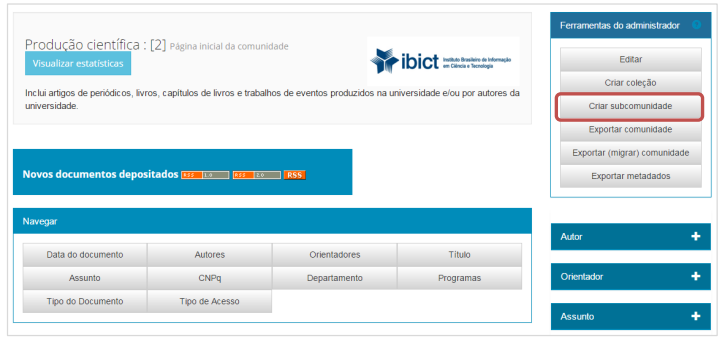
\includegraphics[scale=0.8]{figura/Figura31.png}
                \caption{Criar subcomunidade}
            \label{Rotulo}
        \end{figure}
    
    Passo 2: O processo de criação da subcomunidade é idêntico ao da comunidade. Para acompanhar passo a passo, volte aos itens 3 a 7 da seção 4.1 Criação de comunidade. O processo de estabelecimento de políticas para subcomunidades também é o mesmo das comunidades. A diferença é que você deve acessar a subcomunidade a ser alterada e acessar a respectiva página de edição.
    
    \subsection{Criação de subcomunidade} 
    
    Passo 1: Para editar uma subcomunidade, entre em sua página e clique em <Editar> na caixa de “Ferramentas do administrador”.
    
    \begin{figure}[!htp]
                \centering
                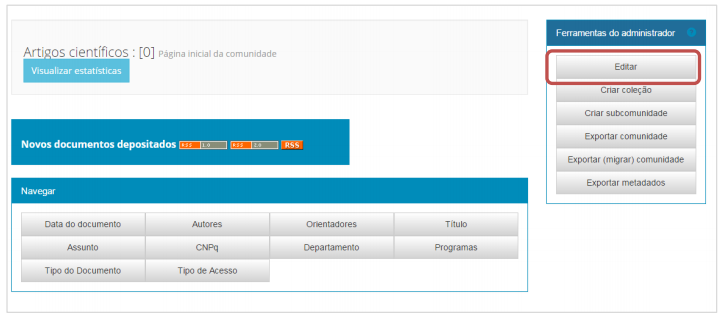
\includegraphics[scale=0.8]{figura/Figura32.png}
                \caption{Criar subcomunidade}
            \label{Rotulo}
        \end{figure}

\newpage  
    \subsection{Criação de coleção}
    
    Passo 1: Para criar uma coleção, entre em uma comunidade ou subcomunidade e clique em <Criar coleção>, nas “Ferramentas do administrador”.
    
    \begin{figure}[!htp]
                \centering
                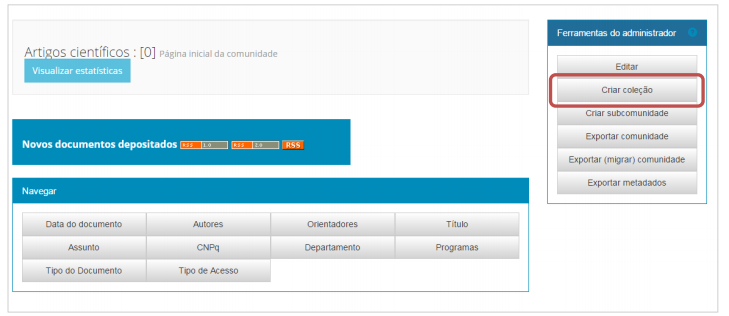
\includegraphics[scale=0.8]{figura/Figura33.png}
                \caption{Criar coleção}
            \label{Rotulo}
        \end{figure}

\newpage
    Passo 2: Descreva a coleção selecionando as características que lhe serão atribuídas. Para selecionar uma característica, basta clicar no quadrado ao lado da frase. Ao finalizar esta fase clique em <Próximo> para continuar o processo de criação da coleção.
    
    \begin{figure}[!htp]
                \centering
                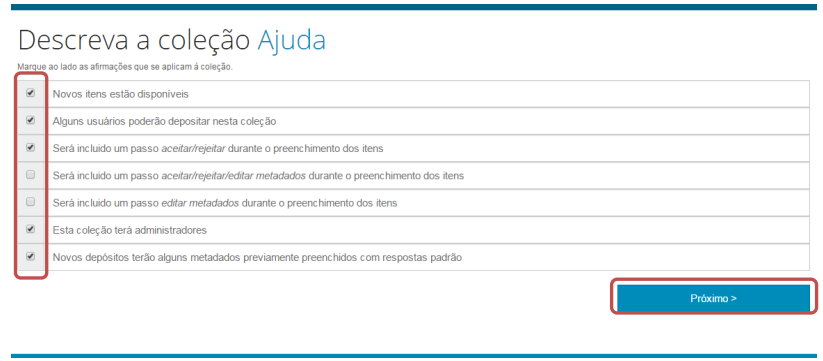
\includegraphics[scale=0.8]{figura/Figura34.png}
                \caption{Descrição da coleção}
            \label{Rotulo}
        \end{figure}
        
    \textbf{\underline{NOTA}}: Essas configurações podem ser editadas posteriormente. 
    
    \singlespacing
    Essas opções formam um fluxo de depósito (workflow) no repositório. Isso significa que elas incluem ou excluem etapas no processo de depósito, que podem ser atribuídas a pessoas diferentes, com permissões diferentes.
    \singlespacing
    
    \textbf{Novos itens estão disponíveis}: os itens inseridos nessa coleção poderão ser visualizados (READ) por usuários anônimos (grupo: Anonymous), ou seja, o padrão para a coleção é ter seus documentos disponíveis ao público, com exceção dos itens restritos e embargados. Se esta opção não estiver marcada, será necessário definir os usuários específicos (ou grupos de usuários) que terão acesso aos itens dessa coleção.
    
    \singlespacing
    
    \textbf{Alguns usuários poderão depositar nesta coleção}: você deverá selecionar quais usuários poderão fazer depósitos nessa determinada coleção. Se esta opção não for marcada ou se nenhum usuário for selecionado, apenas usuários com perfil de administrador poderão realizar o depósito
    
    \singlespacing
    
    \textbf{Será incluído um passo aceitar/rejeitar durante o preenchimento dos itens}: inclui a etapa de avaliação no processo de depósito. Após os usuários depositantes realizarem a submissão de um item, ele não ficará automaticamente disponível no repositório. É preciso que o administrador ou outro usuário/grupo determinado aprove o depósito. Quando esta opção é marcada, é preciso definir os usuários ou grupos responsáveis por aprovar ou rejeitar um depósito. Esses usuários terão acesso ao registro feito pelo depositante e poderão visualizar os metadados preenchidos. Terão a opção de aprovar o depósito (enviando-o para a próxima etapa do fluxo, se houver, ou tornando-o disponível) ou rejeitar o depósito (envia mensagem ao depositante sobre motivo da não aprovação).
    
    \singlespacing
    
    \textbf{Será incluído um passo aceitar/rejeitar/editar metadados durante o preenchimento dos itens}: funciona da mesma maneira que a opção anterior, mas além do usuário responsável pela revisão poder “aprovar” e “rejeitar” um depósito, ele poderá também alterar os seus metadados. Se houver erros a serem corrigidos no depósito, o próprio revisor poderá consertá-los, em vez de solicitar que o depositante os conserte.
    
\newpage
    
    \textbf{Será incluído um passo editar metadados durante o preenchimento dos itens}: novamente, tem o mesmo funcionamento das opções anteriores. É preciso selecionar um usuário ou grupo responsável por revisar os depósitos realizados na coleção. Esses usuários terão a opção de alterar os metadados desse depósito. Após revisar e editar os metadados desejados, os responsáveis podem completar e disponibilizar o depósito, ou seja, tornar o registro disponível para o público.
    
    \singlespacing
    
    \textbf{Esta coleção terá administradores}: caso deseje selecionar usuários específicos para administrarem uma determinada coleção, marque essa opção. Esta opção pode ser usada, por exemplo, para dar autonomia para cada campus da universidade ou para cada faculdade/instituto gerenciar a sua coleção.
    
    \singlespacing
    
    \textbf{Novos depósitos terão alguns metadados previamente preenchidos com respostas padrão}: você pode determinar que certos metadados de uma coleção específica sejam preenchidos sempre com os mesmos valores. Por exemplo, em uma coleção que só receberá artigos científicos, você pode pré-determinar o metadado que registra o tipo de documento como “artigo de periódico” para todos os itens dessa coleção.
    
    \singlespacing
    
    A configuração do fluxo de depósito é explicada no tópico 3.3.2 Estabelecimento de políticas e fluxo de depósito da coleção. 
    
    \singlespacing
    
    Passo 3: Preencha os campos que julgar necessários para descrever a coleção e clique em <Próximo>.
    
    \begin{figure}[!htp]
                \centering
                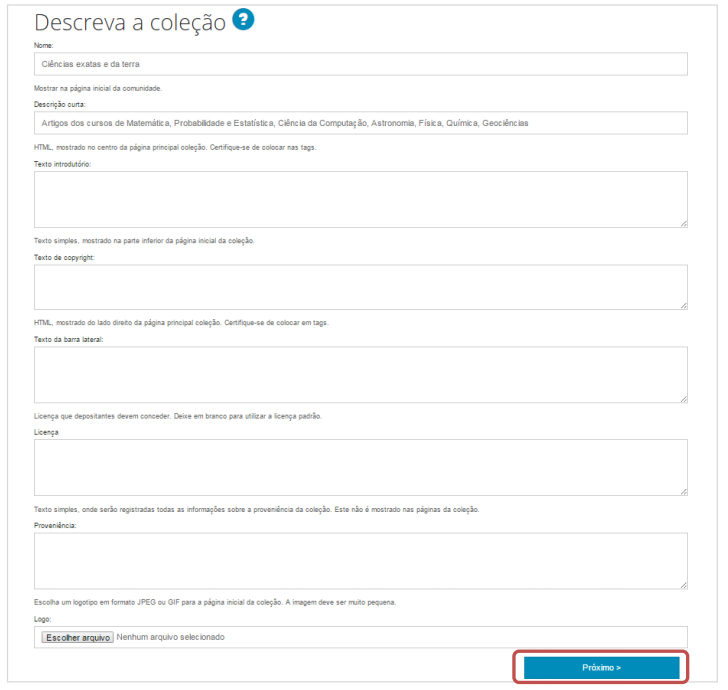
\includegraphics[scale=0.7]{figura/Figura35.png}
                \caption{Descrever a coleção}
            \label{Rotulo}
        \end{figure}

\newpage

    \singlespacing 
     
    \textbullet \hspace{6pt} \textbf{Nome}: informe o nome que será dado à coleção. Exemplo: Ciências exatas e da terra.
     
    \singlespacing
     
    \textbullet \hspace{6pt} \textbf{Descrição curta}: descreva a coleção. Exemplo: Artigos dos cursos de Matemática, Probabilidade e Estatística, Ciência da Computação, Astronomia, Física, Química, Geociências.
    
    \singlespacing
     
    \textbullet \hspace{6pt} \textbf{Texto introdutório (HTML)}: insira um texto sobre a coleção. Permite o uso de tags html que alteram a apresentação do texto. Exemplo: <p><b> Coleção de artigos 34 publicados por alunos e docentes dos cursos de Matemática, Probabilidade e Estatística, Ciência da Computação, Astronomia, Física, Química, Geociências. </b> </p>
    
    \singlespacing
     
    \textbullet \hspace{6pt} \textbf{Texto de copyright}: utilizado para informar os usuários sobre os direitos do autor. É um campo meramente informativo, implica num aviso, estando em conformidade com a política de acesso e de preservação da instituição mantenedora do repositório. Pode ser utilizado para explicar a restrição em coleções de acesso controlado, por exemplo.
    
    \singlespacing
     
    \textbullet \hspace{6pt} \textbf{Texto da barra lateral}: insira outro texto que queira para descrever a comunidade que aparecerá na barra lateral da página da comunidade.
    
    \singlespacing
     
    \textbullet \hspace{6pt} \textbf{Proveniência}: não aparece na página da coleção. Esse campo pode ser utilizado para inserir outras informações relevantes à coleção, sendo que apenas o administrador terá acesso a essas informações no processo de edição da coleção. É utilizado para indicar a origem dos documentos depositados em determinada coleção.
    
    \singlespacing
    
    Passo 4: Se anteriormente você marcou a opção “Alguns usuários poderão depositar nesta coleção”, o próximo passo é a atribuir autorização para o depósito de documentos na coleção, ou seja, selecionar os usuários que poderão adicionar itens a essa coleção.
    
    Clique em <Selecionar usuários> para selecionar usuários individualmente ou <Selecionar grupos> para selecionar grupos de usuários previamente estabelecidos. Após a seleção clique em <Próximo>.
    
    \begin{figure}[!htp]
                \centering
                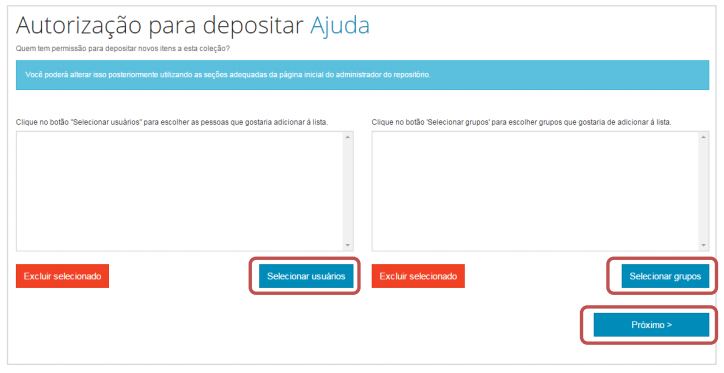
\includegraphics[scale=0.8]{figura/Figura36.png}
                \caption{Permissões de depósito na coleção}
            \label{Rotulo}
        \end{figure}

\newpage

    Passo 5: Se anteriormente você marcou a opção “Esta coleção terá administradores”, o próximo passo é selecionar os usuários ou grupo de usuários que terão permissão de administrador da coleção. Após selecioná-los, clique em <Próximo>
    
    \begin{figure}[!htp]
                \centering
                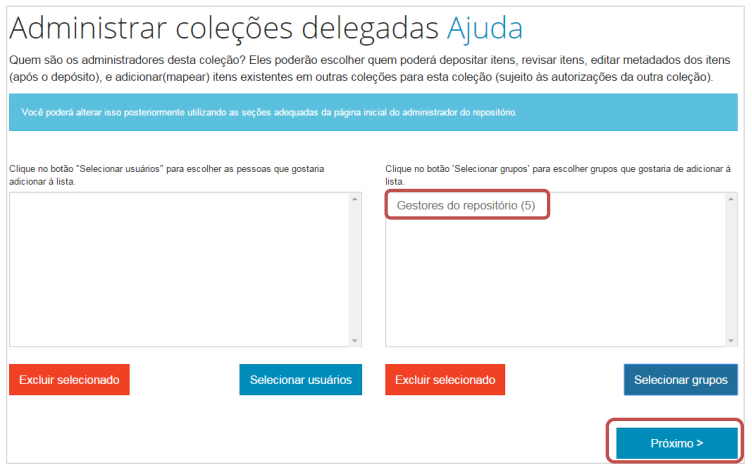
\includegraphics[scale=0.7]{figura/Figura37.png}
                \caption{Permissões de administrador da coleção}
            \label{Rotulo}
        \end{figure}
    
    Passo 6: Se anteriormente você marcou a opção “Novos depósitos terão alguns metadados previamente preenchidos com respostas padrão”, o próximo passo é configurar os campos que terão valores pré-definidos dentro da coleção.
    
    \singlespacing
    
    Escolha o metadado nas caixas de seleção. Insira o valor do campo, ou seja, como ele será preenchido, e a sigla do idioma, de acordo com o padrão adotado. A seguir, clique em Próximo.
    
    \begin{figure}[!htp]
                \centering
                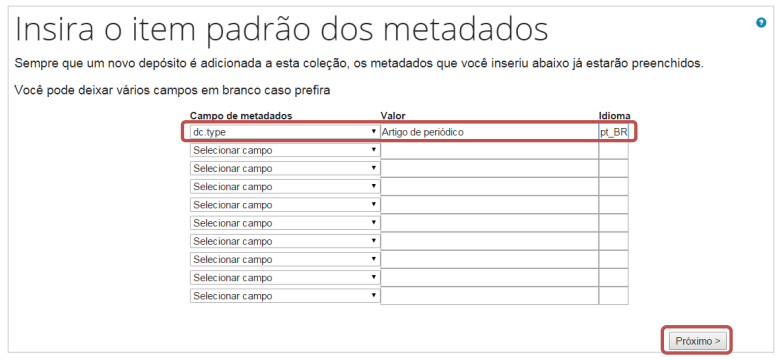
\includegraphics[scale=0.7]{figura/Figura38.png}
                \caption{Configurar metadados pré-definidos}
            \label{Rotulo}
        \end{figure}
        
\newpage

    Passo 7: Finalizada esta etapa, a coleção está criada. A próxima tela que aparecerá é de edição
    da coleção. Nesta tela, é possível alterar todas as informações inseridas nas etapas anteriores ou incluir novas informações. Clique em <Atualizar> para confirmar as alterações.
    
    \begin{figure}[!htp]
                \centering
                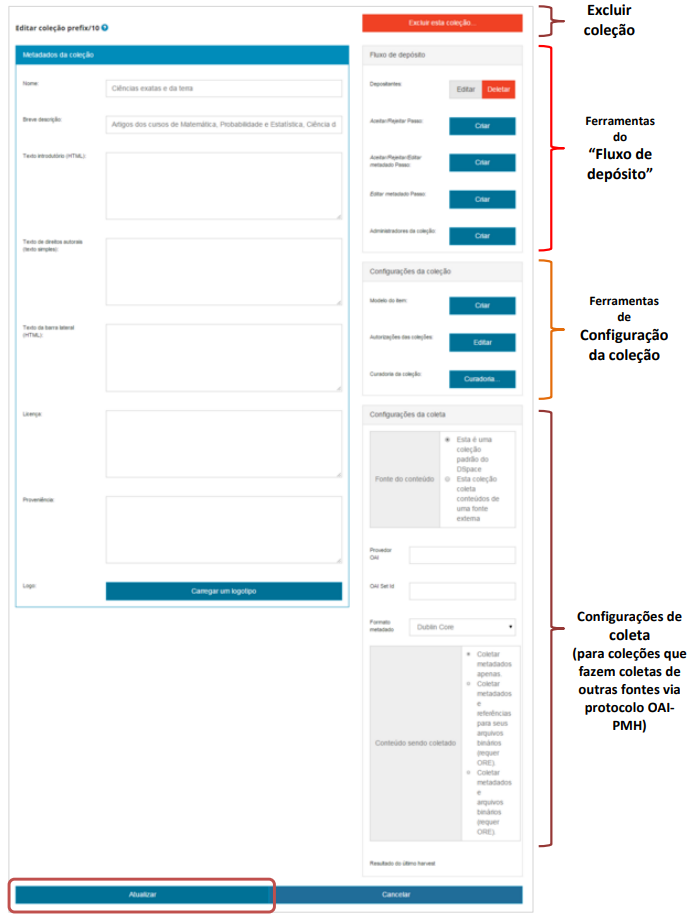
\includegraphics[scale=0.9]{figura/Figura39.png}
                \caption{Página de edição da coleção}
            \label{Rotulo}
        \end{figure}
    
\newpage

    \subsection{Editar coleção}
    
    Passo 1: Para editar as configurações de uma coleção, entre na página da mesma e clique em <Editar>, disponível na caixa de “Ferramentas do administrador”.
    
    \begin{figure}[!htp]
                \centering
                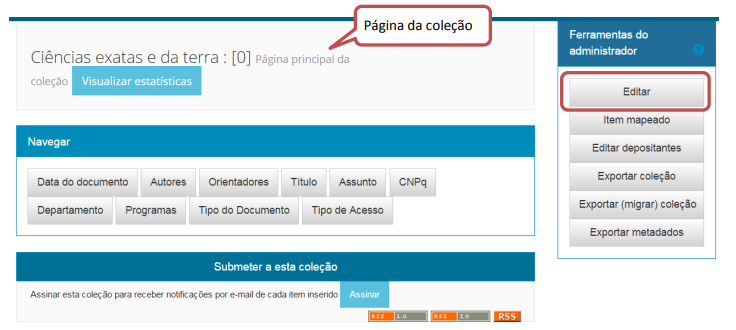
\includegraphics[scale=0.8]{figura/Figura40.png}
                \caption{Editar uma coleção}
            \label{Rotulo}
        \end{figure}
    
    \subsection{Estabelecimento de políticas e fluxo de depósito da coleção}
    
    Há duas formas de estabelecer políticas e configurar o fluxo do depósito de uma coleção. A primeira acontece no ato da criação da coleção (vide tópico 3.3 Criação de coleção). A segunda, na edição de uma coleção já criada.
    
    \singlespacing
    
    Para criar ou alterar alguma permissão estabelecida, vá para a seção de “Fluxo de depósito” na página de edição da coleção. Se você já houver definido uma determinada configuração em outro momento, você terá as opções de editar ou excluir essas configurações. Caso não tenha definido nenhuma configuração, você terá a opção de criar uma nova.
    
    \begin{figure}[!htp]
                \centering
                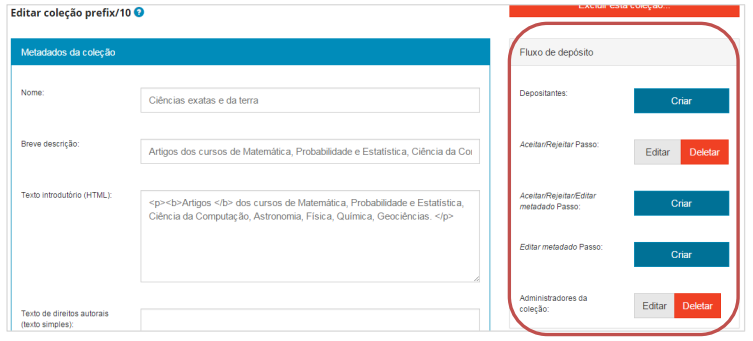
\includegraphics[scale=0.8]{figura/Figura41.png}
                \caption{Editar políticas da coleção}
            \label{Rotulo}
        \end{figure}

\newpage
    
    \textbf{IMPORTANTE}: se você alterar a política de uma coleção que já possui itens, a nova política só valerá para os itens depositados depois da mudança. Os itens existentes permanecerão com as políticas antigas, ou seja, não serão atualizados automaticamente. Para atualizá-los, siga os procedimentos descritos em x.x.x Ferramenta avançada de administração de políticas.
    
    \subsection{Configurar depositantes}
    
    Passo 1: Para determinar os usuários que podem depositar na coleção, clique em “Criar”, caso não tenha definido ainda, ou “Editar”, se você já concedeu permissões anteriormente. Se nenhum usuário ou grupo específico forem selecionados, só os usuários com perfil de “administrador” poderão incluir itens.
    
    \begin{figure}[!htp]
                \centering
                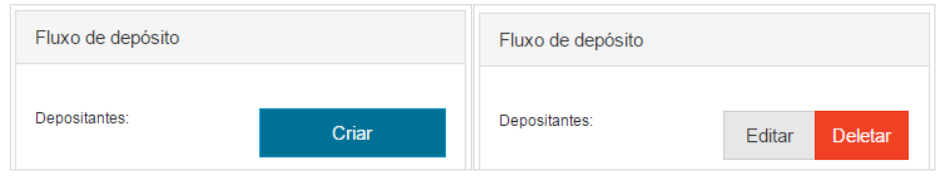
\includegraphics[scale=0.7]{figura/Figura42.png}
                \caption{Configurar depositantes}
            \label{Rotulo}
        \end{figure}

    \singlespacing
    
    Passo 2: Aqui, o processo de selecionar usuários segue o mesmo princípio já apresentado. Clique em “Selecionar usuários” para escolher individualmente as pessoas que poderão fazer depósitos nessa coleção, ou clique em “Selecionar grupos” para dar permissão de depósito a um grupo de usuários. Confirme a ação, clicando em “Atualizar grupo”.
    
    \begin{figure}[!htp]
                \centering
                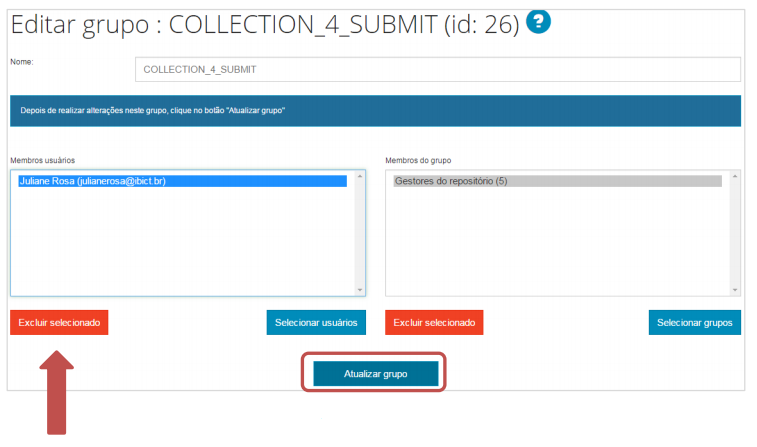
\includegraphics[scale=0.8]{figura/Figura43.png}
                \caption{Selecionar ou excluir depositantes}
            \label{Rotulo}
        \end{figure}

\newpage

    Você também poderá retirar as permissões de usuários e grupos, selecionando-os na lista e clicando em “Excluir selecionado”
    
    \subsection{Aceitar/Rejeitar Passo}
    
    O fluxo de depósito pode ser composto por 3 etapas diferentes: Submissão do item, Avaliação da pertinência do item à coleção e ao repositório (etapa de avaliação), e Revisão dos metadados (etapa de revisão).
    
    \begin{figure}[!htp]
                \centering
                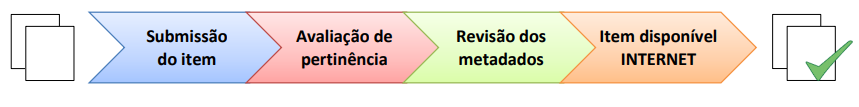
\includegraphics[scale=0.7]{figura/Aceitar-Rejeitar-passo.png}
            \label{Rotulo}
        \end{figure}
    
    Esta é a etapa de avaliação do depósito. Criando esta política, os depósitos realizados só ficarão disponíveis ao público depois de serem aprovados pela(s) pessoa(s) responsável(is). Para definir os usuários ou grupos que farão a avaliação dos itens depositados, clique em “Criar” ou “Editar”.
    
    \begin{figure}[!htp]
                \centering
                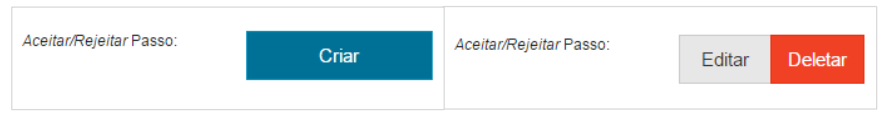
\includegraphics[scale=0.7]{figura/Figura44.png}
                \caption{Configurar etapa de avaliação}
            \label{Rotulo}
        \end{figure}
        
    Clique em “Selecionar usuários” para escolher individualmente as pessoas que irão avaliar os depósitos dessa coleção, ou clique em “Selecionar grupos” para escolher um grupo de usuários avaliadores. Confirme a ação, clicando em “Atualizar grupo”.
    
    \begin{figure}[!htp]
                \centering
                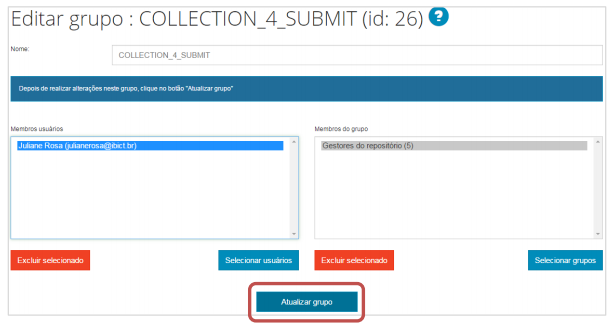
\includegraphics[scale=0.9]{figura/Figura45.png}
                \caption{Selecionar ou excluir avaliadores}
            \label{Rotulo}
        \end{figure}
        
    Esses usuários terão acesso ao registro feito pelo depositante e poderão visualizar os metadados preenchidos. Terão a opção de aprovar ou rejeitar o depósito (envia mensagem ao depositante sobre motivo da não aprovação). Se o fluxo de depósito contiver também a etapa de revisão dos

\newpage

    metadados, ao aprovar um depósito, ele ficará aguardando a execução da revisão. Se não houver a etapa de revisão dos metadados, um depósito aprovado ficará automaticamente disponível ao público geral, isto é, será finalizado.
    
    \subsection{Aceitar/Rejeitar/Editar metadado Passo}
    
    Esta configuração acrescenta duas etapas no fluxo de depósito: avaliação da pertinência e revisão dos metadados, ou seja, consiste em um fluxo de trabalho mais complexo.
    
    \singlespacing
    
    Criando esta política, os depósitos realizados só ficarão disponíveis ao público depois de serem aprovados pelos usuários avaliadores. Selecionando-se essa opção, os usuários avaliadores poderão aprovar ou rejeitar um depósito e também ficarão responsáveis pela revisão dos metadados (poderão não só ver, como editar os metadados dos depósitos realizados).
    
    \singlespacing
    
    Para definir os usuários ou grupos que farão a avaliação e revisão dos metadados dos itens depositados, clique em “Criar” ou “Editar”.
    
    \begin{figure}[!htp]
                \centering
                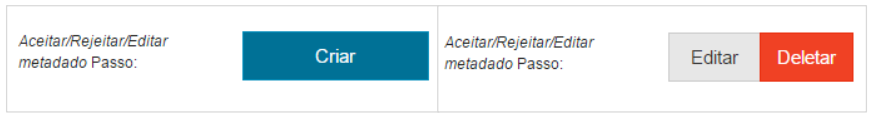
\includegraphics[scale=0.7]{figura/Figura46.png}
                \caption{Configurar fluxo de trabalho completo}
            \label{Rotulo}
        \end{figure}
    
    Clique em “Selecionar usuários” para escolher individualmente as pessoas que irão avaliar e revisar os depósitos dessa coleção, ou clique em “Selecionar grupos” para escolher um grupo de usuários avaliadores/revisores. Confirme a ação, clicando em “Atualizar grupo”.
    
    \begin{figure}[!htp]
                \centering
                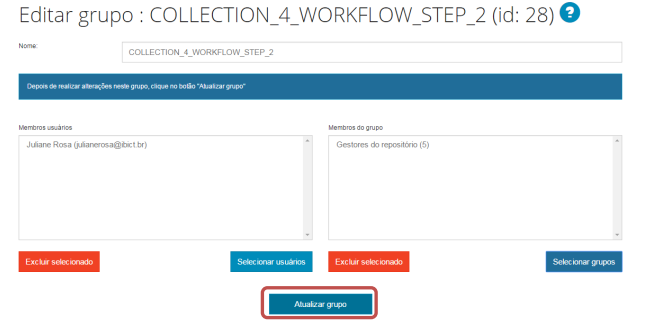
\includegraphics[scale=0.8]{figura/Figura47.png}
                \caption{Selecionar ou excluir avaliadores e revisores}
            \label{Rotulo}
        \end{figure}
    
\newpage

    \subsection{Editar metadado Passo}
    
    Esta é a etapa de revisão de metadados do depósito. Criando esta política, os depósitos realizados só ficarão disponíveis ao público depois de terem seus metadados avaliados pela(s) pessoa(s) responsável(is). Os usuários revisores terão a opção de visualizar e alterar os metadados dos depósitos. Após revisar e/ou editar os metadados desejados, os revisores podem completar o depósito, disponibilizando-o ao público geral.
    
    \singlespacing
    
    Para definir os usuários ou grupos que farão a revisão dos metadados dos itens depositados, clique em “Criar” ou “Editar”.
    
    \begin{figure}[!htp]
                \centering
                \includegraphics[scale=0.6]{figura/Figura48.png}
                \caption{Configurar etapa de revisão de metadados}
            \label{Rotulo}
        \end{figure}
    
    Clique em “Selecionar usuários” para escolher individualmente as pessoas que irão revisar os metadados dos itens depositados nessa coleção, ou clique em “Selecionar grupos” para escolher um grupo de usuários revisores. Confirme a ação, clicando em “Atualizar grupo”.
    
    \begin{figure}[!htp]
                \centering
                \includegraphics[scale=0.8]{figura/Figura49.png}
                \caption{Selecionar revisores dos metadados}
            \label{Rotulo}
        \end{figure}

    \singlespacing
    
    \textbf{Observação}: as três possíveis etapas do fluxo de depósito apresentadas podem ser combinadas de acordo com o contexto e complexidade de cada instituição. Podem ser usadas exclusiva ou cumulativamente, possibilitando que o gestor do repositório delegue tarefas específicas à equipe, atribuindo permissões a apenas um grupo ou pessoa, ou a vários grupos e pessoas.
    
\newpage

\section{Ferramentas do administrador}

\newpage
    
    Para acessar as ferramentas do administrador primeiro você deve ter permissão para isto. Caso você já tenha a permissão, após fazer o login no sistema (vide tópico 1.2 Logar no repositório), clique em <Administrador>.
    
    \begin{figure}[!htp]
                \centering
                \includegraphics[scale=0.7]{figura/Figura50.png}
                \caption{Campo do administrador}
            \label{Rotulo}
        \end{figure}
    
    As ferramentas do administrador são apresentadas nos seguintes menus: <Conteúdo>, <Controle de acesso>, <Estatísticas> e <Configurações gerais>.
    
    \begin{figure}[!htp]
                \centering
                \includegraphics[scale=0.8]{figura/Figura51.png}
                \caption{Ferramentas de administração}
            \label{Rotulo}
        \end{figure}
        
    \subsection{Administrar usuários}

    O menu “Controle de acesso” apresenta um módulo de administração que permite adicionar, excluir e editar o cadastro de usuários do sistema. Caso deseje realizar alguma destas tarefas siga os passos abaixo:
    
    \singlespacing
    
    No menu “Controle de acesso”, selecione <Usuários>.

    \begin{figure}[!htp]
                \centering
                \includegraphics[scale=0.8]{figura/Figura52.png}
                \caption{Administrar usuários}
            \label{Rotulo}
        \end{figure}

\newpage 

    \subsection{Inclusão de novos usuários}
    
    Passo 1: Para adicionar um novo usuário clique em <Adicionar usuário>.
    
    \begin{figure}[!htp]
                \centering
                \includegraphics[scale=0.8]{figura/Figura53.png}
                \caption{Adicionar usuário}
            \label{Rotulo}
        \end{figure}
        
    Passo 2: Preencha as informações solicitadas e para finalizar clique em <Salvar>. Note que o campo “E-mail” virá automaticamente preenchido, no entanto, para o cadastro ser realizado é necessário apagar o texto e incluir um endereço de e-mail válido.

\newpage

    \begin{figure}[!htp]
                \centering
                \includegraphics[scale=0.8]{figura/Figura54.png}
                \caption{Editar usuário}
            \label{Rotulo}
        \end{figure}
    
    Após o preenchimento das informações, o usuário estará cadastrado no sistema. Uma vez registrado, o usuário poderá receber ou perder permissões, como permissão para depositar, permissão para avaliar a pertinência dos depósitos, permissão para revisar os metadados dos depósitos, permissão de administrador etc.
    
    \singlespacing
    
    \textbf{Observação}: Para que o novo usuário receba um e-mail para cadastrar uma senha, deve-se clicar no botão <Redefinir Senha>.

    \subsection{Exclusão de usuários}
    
    Passo 1: Para excluir um usuário já cadastrado no sistema, clique em <Selecionar usuário>.
    
    \begin{figure}[!htp]
                \centering
                \includegraphics[scale=0.8]{figura/Figura55.png}
                \caption{Selecionar usuário}
            \label{Rotulo}
        \end{figure}
    
\newpage

    Passo 2: Selecione o usuário desejado.
    
    \begin{figure}[!htp]
                \centering
                \includegraphics[scale=0.8]{figura/Figura56.png}
                \caption{Selecionar usuário}
            \label{Rotulo}
        \end{figure}

\newpage

    Passo 3: Confira se o usuário selecionado é de fato o que deve ser excluído e depois clique em <Excluir>
    
    \begin{figure}[!htp]
                \centering
                \includegraphics[scale=0.8]{figura/Figura57.png}
                \caption{Excluir usuário}
            \label{Rotulo}
        \end{figure}
    
    \textcolor{red}{ATENÇÃO}: \textbf{Não} é possível excluir um usuário que tenha depósitos ou tarefas pendentes. Neste caso é possível somente bloquear seu acesso ao se desmarcar o botão \textbf{<Pode Entrar>}.
    
    \begin{figure}[!htp]
                \centering
                \includegraphics[scale=0.8]{figura/Figura58.png}
                \caption{Bloquear acesso do usuário}
            \label{Rotulo}
        \end{figure}

\newpage

    \subsection{Editar informações dos usuários cadastrados}
    
    Passo 1: Para editar as informações cadastradas sobre os usuários clique em <Selecionar usuário>
    
    \begin{figure}[!htp]
                \centering
                \includegraphics[scale=0.8]{figura/Figura59.png}
                \caption{Selecionar usuário para editar}
            \label{Rotulo}
        \end{figure}

    Passo 2: Selecione o usuário desejado.
    
    \begin{figure}[!htp]
                \centering
                \includegraphics[scale=0.8]{figura/Figura60.png}
                \caption{Selecionar usuário para editar}
            \label{Rotulo}
        \end{figure}

\newpage

    Passo 3: Clique em <Editar>.
    
    \begin{figure}[!htp]
                \centering
                \includegraphics[scale=0.8]{figura/Figura61.png}
                \caption{Editar usuário selecionado}
            \label{Rotulo}
        \end{figure}
    
    Passo 4: Altere as informações necessárias e depois clique em <Salvar>.
    
    \begin{figure}[!htp]
                \centering
                \includegraphics[scale=0.7]{figura/Figura62.png}
                \caption{Editar usuário selecionado}
            \label{Rotulo}
        \end{figure}

\newpage

    \subsection{Administrar grupos de usuários}
    
    Este módulo de administração permite adicionar, excluir e editar grupos de usuários do sistema. Caso deseje realizar alguma destas tarefas, siga os passos abaixo:
    
    \singlespacing
    
    Passo 1: Nas ferramentas de administração, acesse o menu “Controle de acesso” e clique em <Grupos>.
    
    \begin{figure}[!htp]
                \centering
                \includegraphics[scale=0.8]{figura/Figura63.png}
                \caption{Administrar grupos de usuários}
            \label{Rotulo}
        \end{figure}
    
    \subsection{Criar grupos de usuários}
    
    Passo 1: Para criar um novo grupo de usuários clique em <Criar novo grupo>.
    
    \begin{figure}[!htp]
                \centering
                \includegraphics[scale=0.8]{figura/Figura64.png}
                \caption{Administrar grupos de usuários}
            \label{Rotulo}
        \end{figure}
\newpage
    
    Passo 2: Edite o nome do grupo no campo “Nome”. Note que um nome automático é dado para o grupo criado. Caso este nome não seja alterado o grupo ficará com o nome que foi gerado automaticamente.
    
    \begin{figure}[!htp]
                \centering
                \includegraphics[scale=0.8]{figura/Figura65.png}
                \caption{Administrar grupos de usuários}
            \label{Rotulo}
        \end{figure}
    
    Passo 3: Selecione membros para participar do grupo. Para tanto, clique em <Selecionar usuários> para escolher participantes individualmente e/ou clique em <Selecionar grupos> para selecionar grupos de usuários. Finalizada a seleção, clique em <Atualizar grupo>.
    
    \begin{figure}[!htp]
                \centering
                \includegraphics[scale=0.7]{figura/Figura66.png}
                \caption{Selecionar membros ou grupos de usuários}
            \label{Rotulo}
        \end{figure}
        
\newpage
    
    \subsection{Excluir grupos de usuários}
    
    Passo 1: Para excluir um grupo de usuários basta clicar em <Excluir> ao lado do nome do grupo.
    
    \begin{figure}[!htp]
                \centering
                \includegraphics[scale=0.8]{figura/Figura67.png}
                \caption{Excluir grupo de usuários}
            \label{Rotulo}
        \end{figure}
    
    Passo 2: Ao solicitar a exclusão de um grupo, será pedido que você confirme a ação. Caso esteja seguro da exclusão do grupo clique em <Excluir>.
    
    \begin{figure}[!htp]
                \centering
                \includegraphics[scale=0.8]{figura/Figura68.png}
                \caption{Confirmação de exclusão de grupo}
            \label{Rotulo}
        \end{figure}

\newpage

    \subsection{Editar grupo de usuários}
    
    Passo 1: Para editar as configurações de um grupo já criado, clique em <Editar> ao lado do nome do grupo em que pretende realizar as alterações. 
    
    \begin{figure}[!htp]
                \centering
                \includegraphics[scale=0.8]{figura/Figura69.png}
                \caption{Editar grupo de usuários}
            \label{Rotulo}
        \end{figure}
        
    Passo 2: Na edição do grupo, você poderá incluir e/ou excluir usuários ou grupos. Após finalizadas as edições, clique em <Atualizar grupo>.
    
    \begin{figure}[!htp]
                \centering
                \includegraphics[scale=0.7]{figura/Figura70.png}
                \caption{Incluir e excluir usuários no grupo de usuários}
            \label{Rotulo}
        \end{figure}

\newpage
    
    \subsection{Administrar políticas de autorização}
    
    Para gerenciar as políticas de autorização das comunidades, coleções e itens do repositório, use as ferramentas da página <Autorização>, no menu <Controle de acesso>.
    
    \begin{figure}[!htp]
                \centering
                \includegraphics[scale=0.7]{figura/Figura71.png}
                \caption{Gerenciar políticas de autorização}
            \label{Rotulo}
        \end{figure}
    
    Selecione uma das opções de administração de políticas.
    
    \begin{figure}[!htp]
                \centering
                \includegraphics[scale=0.7]{figura/Figura72.png}
                \caption{Opções para administrar políticas de autorização}
            \label{Rotulo}
        \end{figure}
    
    \subsection{Gerenciar políticas de uma comunidade}
    
    Passo 1: Para visualizar, criar ou editar as políticas de uma comunidade clique em <Gerenciar políticas de uma comunidade>.

\newpage

    Note que também é possível realizar essas alterações acessando a página da comunidade de interesse e clicando em <Editar> (vide tópico 4.2 Editar comunidade).
    
    \begin{figure}[!htp]
                \centering
                \includegraphics[scale=0.7]{figura/Figura73.png}
                \caption{Gerenciar políticas de uma comunidade}
            \label{Rotulo}
        \end{figure}
    
    Passo 2: Selecione a comunidade ou subcomunidade desejada e clique em <Editar políticas>.
    
    \begin{figure}[!htp]
                \centering
                \includegraphics[scale=0.8]{figura/Figura74.png}
                \caption{Editar política de uma comunidade selecionada}
            \label{Rotulo}
        \end{figure}
    
    Passo 3: Selecione a política que você deseja editar, clicando em <Editar> ao lado da mesma ou crie uma nova política clicando em <Adicionar nova política>. 
    
    \begin{figure}[!htp]
                \centering
                \includegraphics[scale=0.8]{figura/Figura75.png}
                \caption{Editar ou criar uma política para uma comunidade}
            \label{Rotulo}
        \end{figure}

\newpage
    
    Passo 4: o passo seguinte, tanto durante a edição ou criação de uma política, consiste em escolher o grupo que receberá a nova permissão e a respectiva ação que esse grupo de usuários poderá executar. Clique em <Salvar> para manter as alterações ou em <Cancelar> para voltar à página anterior.
    
    \begin{figure}[!htp]
                \centering
                \includegraphics[scale=0.8]{figura/Figura76.png}
                \caption{Selecionar novas permissões para a comunidade}
            \label{Rotulo}
        \end{figure}
    
    Informações sobre as permissões:
    
    \singlespacing
    
    READ – permissão de visualização/leitura dos registros; \\
    WRITE – permissão de edição dos itens da comunidade; \\
    ADD – permissão para adicionar/depositar itens dentro da comunidade; \\
    REMOVE – permissão para remover/excluir itens da comunidade; \\
    ADMIN – permissão de administrador da comunidade (possui todas as permissões).
    
    \singlespacing
    
    Passo 5: Para excluir uma política, clique em <Excluir> no campo da política que pretende deletar. Confira se realmente deseja apagar a política em questão, pois o sistema não exige confirmação e a exclusão não poderá ser desfeita.
    
    \begin{figure}[!htp]
                \centering
                \includegraphics[scale=0.8]{figura/Figura77.png}
                \caption{Excluir políticas da comunidade}
            \label{Rotulo}
        \end{figure}

\newpage
    
    \subsection{Gerenciar políticas de uma coleção}
    
    Passo 1: Para visualizar, criar ou editar as políticas de uma coleção clique em <Gerenciar políticas de uma coleção>.
    
    Note que também é possível realizar essas alterações acessando a página da coleção de interesse e clicando em <Editar> (vide tópico 4.7 Editar coleção).
    
    \begin{figure}[!htp]
                \centering
                \includegraphics[scale=0.8]{figura/Figura78.png}
                \caption{Gerenciar políticas de uma coleção}
            \label{Rotulo}
        \end{figure}
    
    Passo 2: Selecione a coleção desejada e clique em <Editar políticas>.
    
    \begin{figure}[!htp]
                \centering
                \includegraphics[scale=0.8]{figura/Figura79.png}
                \caption{Selecionar coleção para editar política}
            \label{Rotulo}
        \end{figure}
        
    Para realizar as alterações, repita os passos 3, 4 e 5 da seção anterior.

\newpage

    \subsection{Gerenciar políticas de um item}
    
    Passo 1: Para visualizar, criar ou editar as políticas de um item clique em <Gerenciar políticas de um item>.
    
    \singlespacing
    
    Note que também é possível realizar essas alterações acessando o registro do item, navegando pelas comunidades e coleções ou usando a ferramenta de busca (vide tópico 5.14 Editar itens depositados no repositório).
    
    \begin{figure}[!htp]
                \centering
                \includegraphics[scale=0.8]{figura/Figura80.png}
                \caption{Gerenciar políticas de um item}
            \label{Rotulo}
        \end{figure}
    
    \singlespacing
    
    Passo 2: informe o número identificador do item. Veja mais sobre como encontrar o identificador do item no tópico 5.14 Editar itensdepositados no repositório.
    
    \begin{figure}[!htp]
                \centering
                \includegraphics[scale=0.8]{figura/Figura81.png}
                \caption{Informe o número identificador do item}
            \label{Rotulo}
        \end{figure}
    
    Passo 3: serão apresentadas as políticas relacionadas ao item. Para saber mais sobre a edição dessas políticas, acesse o tópico 4.4.8 Editar autorizações dos itens.
    
     \begin{figure}[!htp]
                \centering
                \includegraphics[scale=0.8]{figura/Figura82.png}
                \caption{Gerenciar políticas do item}
            \label{Rotulo}
        \end{figure}

\newpage

    \subsection{Ferramenta avançada de administração de políticas}
    
    Esta ferramenta é usada para definir e excluir políticas para todos os itens (refere-se ao conjunto metadados + arquivos) ou bitstreams (arquivos digitais) pertencentes a uma coleção. Por exemplo, se você possuir uma coleção com vários itens e precisar mudar as permissões de acesso à essa coleção. Se você alterar a política padrão de uma coleção que já possui itens, essa nova política só valerá para itens incluídos a partir da mudança, ou seja, os itens existentes permanecerão sob a antiga política. Como os itens existentes não terão suas políticas atualizadas automaticamente é necessário mudar as suas permissões usando esta ferramenta.
    
    \singlespacing
    
    Passo 1: Para acessá-la, clique em <Ferramenta de administração política>.
    
    \begin{figure}[!htp]
                \centering
                \includegraphics[scale=0.8]{figura/Figura83.png}
                \caption{Ferramenta de administração de política}
            \label{Rotulo}
        \end{figure}
    
    \singlespacing
    
    Passo 2: A ferramenta permite a configuração de 4 elementos:
    
    \singlespacing
    
    \textbullet \hspace{6pt} Selecione na lista a coleção a qual deseja atribuir ou remover a permissão; \\
    \textbullet \hspace{6pt} Selecione o elemento que terá a permissão editada (item ou bitstream); \\
    \textbullet \hspace{6pt} Selecione o grupo de usuários que receberá/perderá a permissão; 
    \textbullet \hspace{6pt} Selecione a permissão que o grupo terá sobre o elemento.
    
    \begin{figure}[!htp]
                \centering
                \includegraphics[scale=0.6]{figura/Figura84.png}
                \caption{Gerenciar políticas avançadas}
            \label{Rotulo}
        \end{figure}
    
\newpage
    
    Exemplo de uso 1: digamos que você queira dar a um determinado grupo privilegiado (grupo Professores) uma permissão de acesso de leitura a todos os arquivos (bitstreams) de uma coleção restrita. Você iria indicar a coleção, selecionar a opção <Professores> na lista “Grupo”, <bitstream> na lista “Tipo de conteúdo”, <READ> na lista “Ação”, e depois clicar em <Adicionar política>.
    
    \subsection{Editar itens depositados no repositório}
    
    Este modo de edição do item permite que sejam adicionados novos campos que não foram preenchidos anteriormente e excluir campos existentes do registro. Há duas maneiras de acessar a página de edição de um item: a) navegar até o item, por meio das comunidades e coleções ou usando a ferramenta de busca; b) por meio do menu <Itens>, nas ferramentas de administração.
    
    \singlespacing
    
    Passo 1: Para editar os itens depositados no repositório, acesse “Conteúdo” e clique em <Itens>, no menu do Administrador. 
    
    \begin{figure}[!htp]
                \centering
                \includegraphics[scale=0.8]{figura/Figura85.png}
                \caption{Administrar itens}
            \label{Rotulo}
        \end{figure}
    
    Passo 2: Para editar um item, por meio desse menu, será necessário informar o identificador do registro no campo adequado e clicar em <Buscar>. O identificador pode ser o Handle ou o ID interno
    
    \begin{figure}[!htp]
                \centering
                \includegraphics[scale=0.8]{figura/Figura86.png}
                \caption{Editar um item}
            \label{Rotulo}
        \end{figure}
    
\newpage
    
    \underline{Como encontrar o identificador}: O identificador de um item é um número que aparece em sua descrição. É dado automaticamente pelo sistema no momento do seu registro.
    
    \begin{figure}[!htp]
                \centering
                \includegraphics[scale=0.8]{figura/Figura87.png}
                \caption{Identificador URI}
            \label{Rotulo}
        \end{figure}
    
    Note que o número que deverá ser informado para a edição do item é somente o número identificador do item, apresentado no final do campo URI. 
    
    \begin{figure}[!htp]
                \centering
                \includegraphics[scale=0.8]{figura/Figura88.png}
                \caption{Identificador do item = último número do URI}
            \label{Rotulo}
        \end{figure}

\newpage
    
    Neste exemplo, o número que deverá ser informado é o dígito “13”. Isto porque no campo Handle os outros algarismos já vêm preenchidos por constituírem um número padrão.
    
    \begin{figure}[!htp]
                \centering
                \includegraphics[scale=0.8]{figura/Figura89.png}
                \caption{Inserir identificador do item}
            \label{Rotulo}
        \end{figure}
    
    \singlespacing
    
    Passo 3: Ao buscar o item, você acessará sua página de edição. Nesta página, é possível visualizar, editar, acrescentar e excluir metadados do registro. Além disso, é possível excluir o registro, movê-lo para outra coleção e mudar as permissões de acesso aos itens.
    
    \begin{figure}[!htp]
                \centering
                \includegraphics[scale=0.7]{figura/Figura90.png}
                \caption{Página de edição do registro}
            \label{Rotulo}
        \end{figure}
    
\newpage
    
    Nota: para salvar qualquer mudança feita, é necessário clicar em “Atualizar”, no final da página de edição. Para cancelar as alterações, clique em “Cancelar”.
    
    \begin{figure}[!htp]
                \centering
                \includegraphics[scale=0.8]{figura/Figura91.png}
                \caption{Salvar ou cancelar mudanças}
            \label{Rotulo}
        \end{figure}
    
    \subsection{Excluir metadado do registro}
    
    \singlespacing
    
    Passo 1: Para excluir um campo de metadado, clique na figura da <lixeira>, ao lado do campo desejado. Confira se o campo que deseja excluir está correto, pois o sistema não exige confirmação antes de apagar o metadado e não há como desfazer a operação
    
    \begin{figure}[!htp]
                \centering
                \includegraphics[scale=0.7]{figura/Figura92.png}
                \caption{Excluir metadados do registro}
            \label{Rotulo}
        \end{figure}
    
    \subsection{Editar uma informação do registro}
    
    Passo 1: Para editar o conteúdo de um determinado campo basta alterar seu texto na coluna “Valor”. Após realizar as alterações, clique em “Atualizar” no fim da página, para salvar as mudanças, ou “Cancelar” para desfazer as alterações.
    
    \begin{figure}[!htp]
                \centering
                \includegraphics[scale=0.7]{figura/Figura93.png}
                \caption{Editar um campo do registro}
            \label{Rotulo}
        \end{figure}
    
    \subsection{Editar uma informação do registro}
    
    
    Passo 1: Para adicionar um novo campo, navegue pela página até o último campo apresentado.
    Abaixo do último campo preenchido, há uma caixa de seleção. Nessa caixa, escolha o metadado
    adequado, preencha-o no campo “Valor” com as informações que deseja adicionar ao registro,
    preencha o campo “Idioma” com “pt\_BR” (sem as aspas) e clique na figura com o sinal de adição.
    
    \begin{figure}[!htp]
                \centering
                \includegraphics[scale=0.7]{figura/mais.png}
            \label{Rotulo}
        \end{figure}

\newpage

    \begin{figure}[!htp]
                \centering
                \includegraphics[scale=0.7]{figura/Figura94.png}
                \caption{Adicionar metadado ao registro}
            \label{Rotulo}
        \end{figure}
    
    \subsection{Adicionar novos documentos ao registro}
    
    Passo 1: Alguns documentos podem ser compostos por mais de um arquivo digital. Nesses casos, para adicionar um novo arquivo ao registro, navegue até a área “Bitstreams”, no final da página de edição, e clique em <Adicionar Bitstream>.
    
    \begin{figure}[!htp]
                \centering
                \includegraphics[scale=0.7]{figura/Figura95.png}
                \caption{Adicionar novo documento ao registro}
            \label{Rotulo}
        \end{figure}

\newpage
    
    Passo 2: Selecione o arquivo desejado, clicando em <Escolher arquivo>.
    
    \begin{figure}[!htp]
                \centering
                \includegraphics[scale=0.7]{figura/Figura96.png}
                \caption{Escolher arquivo binário}
            \label{Rotulo}
        \end{figure}
    
    Passo 3: Navegue pelas pastas de arquivos de seu computador e selecione o arquivo que deseja adicionar ao registro.
    
    \begin{figure}[!htp]
                \centering
                \includegraphics[scale=0.7]{figura/Figura97.png}
                \caption{Selecionar local do arquivo}
            \label{Rotulo}
        \end{figure}
    
    Passo 4: Após ter selecionado o arquivo clique em <Carregar>.
    
    \begin{figure}[!htp]
                \centering
                \includegraphics[scale=0.7]{figura/Figura98.png}
                \caption{Carregar arquivo binário}
            \label{Rotulo}
        \end{figure}

\newpage
    
    Passo 5: Concluídas todas as alterações desejadas, clique em <Atualizar>. Caso queira cancelar as alterações feitas clique em <Cancelar>.
    
    \begin{figure}[!htp]
                \centering
                \includegraphics[scale=0.8]{figura/Figura99.png}
                \caption{Carregar arquivo binário}
            \label{Rotulo}
        \end{figure}
    
    \subsection{Excluir item}
    
    Passo 1: Para excluir um item registrado no sistema você tem duas opções: <Excluir> e <Excluir definitivamente>. Selecione a opção desejada e confirme a ação.
    
    \singlespacing
     
     \textbf{Excluir}: o item não é apagado, e sim “retirado”. O registro fica restrito, apenas pessoas autorizadas poderão acessá-lo. Itens retirados poderão ser reativados ou poderão ser excluídos definitivamente, mediante aprovação de usuários com esta permissão.
     
     \singlespacing
     
    \textbf{Excluir definitivamente}: o item é imediatamente apagado do repositório. Não é possível  recuperar um item excluído definitivamente.
    
    \begin{figure}[!htp]
                \centering
                \includegraphics[scale=0.8]{figura/Figura100.png}
                \caption{Excluir item}
            \label{Rotulo}
        \end{figure}

\newpage

    Passo 2: \textbf{Excluir}. Se optar pela ação de <Excluir>, uma tela de confirmação da retirada do item irá surgir. Você pode confirmar a exclusão, clicando em <Retirar>, ou cancelar a exclusão, clicando em <Cancelar>.
    
    \begin{figure}[!htp]
                \centering
                \includegraphics[scale=0.8]{figura/Figura101.png}
                \caption{Confirmar retirada do item}
            \label{Rotulo}
        \end{figure}
    
    Note que os itens retirados da coleção ou comunidade ficam invisíveis ao público, mas ainda podem ser acessados pelos usuários ou grupo de usuários que possuem a devida permissão. Os itens retirados podem ser visualizados por meio do menu <\textbf{Itens retirados}>, nas Ferramentas de administração. Esses itens podem ser restabelecidos à coleção, se desejado.

\newpage

    \begin{figure}[!htp]
                \centering
                \includegraphics[scale=0.8]{figura/Figura102.png}
                \caption{Acessar itens retirados}
            \label{Rotulo}
        \end{figure}
    
    Passo 2: \textbf{Excluir definitivamente}. Se optar pela ação de <Excluir definitivamente>, uma tela de confirmação da exclusão do item irá surgir. Essa opção é definitiva e o item não poderá ser recuperado novamente. Você pode confirmar a eliminação do item, clicando em <Excluir>, ou cancelar a exclusão, clicando em <Cancelar>.
    
    \begin{figure}[!htp]
                \centering
                \includegraphics[scale=0.7]{figura/Figura103.png}
                \caption{Excluir item definitivamente}
            \label{Rotulo}
        \end{figure}

\newpage

    \subsection{Mover um item para outra coleção}
    
    É possível mover um item de uma coleção para outra, um item de cada vez. \\
    
    Passo 1: Para transferir um item de uma coleção para outra, clique em <Mover item>.
    
    \begin{figure}[!htp]
                \centering
                \includegraphics[scale=0.8]{figura/Figura104.png}
                \caption{Mover um item para outra coleção}
            \label{Rotulo}
        \end{figure}
    
    Passo 2: Selecione o novo destino do item dentre as opções apresentadas na lista “Mover para coleção”.
    
    \singlespacing
    
    Quando um item é movido de uma coleção para outra, ele levará suas permissões com ele, ou seja, manterá as autorizações atuais. Caso queira que o item assuma a política padrão da coleção de destino, marque o campo “Manter o padrão de políticas da coleção de destino”. Ao marcar essa opção, atente-se para que a política da nova coleção não substitua as restrições de acesso do item, como acesso embargado, por exemplo. Por fim, clique em <Mover>.
    
     \begin{figure}[!htp]
                \centering
                \includegraphics[scale=0.8]{figura/Figura105.png}
                \caption{Escolher coleção para mover o item selecionado}
            \label{Rotulo}
        \end{figure}

\newpage

    \subsection{Tornar item privado}
    
    Um item privado não tem os metadados nem os arquivos disponibilizados ao público. Apenas os administradores do repositório e pessoas autorizadas poderão acessá-lo.
    
    \singlespacing
    
    Passo 1: Caso necessite restringir o acesso a um determinado item, clique em <Tornar item privado>.
    
    \begin{figure}[!htp]
                \centering
                \includegraphics[scale=0.7]{figura/Figura106.png}
                \caption{Tornar item privado}
            \label{Rotulo}
        \end{figure}
    
    Passo 2: Uma página de confirmação será apresentada. Confira se o item está correto e clique em <Restringir acesso ao item> para torná-lo privado, ou em <Cancelar> para voltar a página anterior.
    
    \begin{figure}[!htp]
                \centering
                \includegraphics[scale=0.7]{figura/Figura107.png}
                \caption{Confirmar ou cancelar restrição do item}
            \label{Rotulo}
        \end{figure}
        
\newpage

    Note que os itens privados ficam invisíveis ao público, mas ainda podem ser acessados pelos usuários ou grupo de usuários que possuem a devida permissão. Os itens privados podem ser visualizados por meio do menu <\textbf{Itens privados}>, nas Ferramentas de administração. É possível torná-los públicos novamente, se desejado
    
    \begin{figure}[!htp]
                \centering
                \includegraphics[scale=0.7]{figura/Figura108.png}
                \caption{Acessar itens privados}
            \label{Rotulo}
        \end{figure}
    
    \subsection{Editar autorizações dos itens}
    
    É possível visualizar e alterar as políticas (permissões) de cada item, individualmente, na página “Editar item”. \\
    
    Para acessar as políticas do item, clique em <Autorizações dos itens>.
    
    \begin{figure}[!htp]
                \centering
                \includegraphics[scale=0.7]{figura/Figura109.png}
                \caption{Editar autorizações do item}
            \label{Rotulo}
        \end{figure}

\newpage

    A página seguinte apresenta todas as permissões que envolvem o item. As políticas são divididas em: <Políticas por item>, <Políticas por Bundle Original> e <Políticas por Bundle License>.
    
    \begin{figure}[!htp]
                \centering
                \includegraphics[scale=0.7]{figura/Figura110.png}
                \caption{Políticas por item}
            \label{Rotulo}
        \end{figure}
        
    Um item é composto por um conjunto de metadados e objetos digitais. Os objetos digitais são os arquivos depositados no repositório (p. ex., arquivo PDF de um artigo) e os arquivos das licenças associadas ao documento (p. ex., arquivo de texto da licença Creative Commons).
    
    \singlespacing
    
    Os objetos digitais que compõem o item são agrupados em pacotes chamados “bundles”. Há dois tipos de bundles, um que reúne os documentos depositados (Bundle original) e outro que reúne os arquivos das licenças associadas ao item (Bundle License).
    
    \begin{figure}[!htp]
                \centering
                \includegraphics[scale=0.7]{figura/Figura111.png}
                \caption{Estrutura do item}
            \label{Rotulo}
        \end{figure}

\newpage
    
    É possível, portanto, estabelecer uma permissão geral para o item, que será aplicada a todos os seus elementos: metadados, licenças e bitstreams (arquivos); ou estabelecer permissões específicas para cada objeto digital que faz parte de um item. 
    
    \subsection{Política por item}
    
    Para adicionar, alterar ou excluir uma permissão que vale para todos os elementos do item (metadados e objetos digitais), clique na opção correspondente na seção “Políticas por item”.
    
    \begin{figure}[!htp]
                \centering
                \includegraphics[scale=0.8]{figura/Figura112.png}
                \caption{Políticas do item}
            \label{Rotulo}
        \end{figure}
    
    Passo 1: Clique em <Adicionar nova política> para criar novas permissões de acesso ao item. Na página seguinte, escolha o grupo de usuários e a ação que o grupo poderá executar. Clique em <Salvar> para criar a política, ou em <Cancelar> para voltar à página anterior.
    
    \begin{figure}[!htp]
                \centering
                \includegraphics[scale=0.8]{figura/Figura113.png}
                \caption{Editar políticas do item}
            \label{Rotulo}
        \end{figure}
        
\newpage

    Informações sobre as permissões:
    
    \singlespacing
    
    READ – permissão de visualização/leitura do item; \\
    WRITE – permissão de alteração do item, tanto dos objetos digitais quanto dos metadados. \\
    ADD – permissão para adicionar objetos digitais ao bundle do item. \\
    REMOVE - permissão para excluir objetos digitais do bundle do item. \\
    ADMIN – permissão de administrador do item. Inclui todas as permissões anteriores.
    
    Passo 2: Clique em <Editar> para alterar uma política existente. O processo é o mesmo do passo anterior, selecione o grupo e a ação a ser executada por ele. Clique em <Salvar> para manter as alterações, ou em <Cancelar> para voltar à página anterior.
    
    \singlespacing
    
    Passo 3: Clique em <Excluir> para apagar uma política existente. Confira se a política selecionada é realmente aquela que você deseja excluir, pois o sistema não exige confirmação para concluir a exclusão e não é possível desfazer essa operação.
    
    \subsection{Políticas por Bundle original}
    
    \singlespacing
    
    Para adicionar, alterar ou excluir uma permissão que vale apenas para os arquivos depositados em um item, clique na opção correspondente na seção “Políticas por Bundle Original”. As opções e os procedimentos são os mesmos da seção anterior.
    
    \singlespacing
    
    Note que há dois níveis de configuração de políticas para os objetos digitais depositados:
    
    \singlespacing
    
    \textbullet \hspace{6pt} É possível adotar uma política que valha para todos os arquivos que fazem parte do item, ou seja, uma política para o pacote (bundle) de documentos depositados. 
    
    \singlespacing
    
    \textbullet \hspace{6pt} É possível adotar uma política individual para cada arquivo que compõe o item. Essa ferramenta é útil em casos, por exemplo, de substituição de um arquivo por outro, sendo que o antigo não será apagado do repositório, apenas ficará restrito.

    \begin{figure}[!htp]
                \centering
                \includegraphics[scale=0.7]{figura/Figura114.png}
                \caption{Editar políticas do bundle}
            \label{Rotulo}
        \end{figure}

    Note que a prevalência das políticas ocorre de forma hierárquica, valendo sempre a de menor hierarquia, ou seja, uma permissão dada a um elemento superior não se sobrepõe à permissão dada a um elemento inferior
    
    \singlespacing
    
    Nesse caso, uma política atribuída ao item não prevalece sobre a política atribuída ao bundle. Da  mesma maneira, uma política atribuída ao arquivo digital (bitstream) não é substituída por uma política atribuída aos níveis maiores (bundle e item).

\newpage

    \subsection{Política por Bundle License}
    
    Para adicionar, alterar ou excluir uma permissão que vale apenas para as licenças associadas aos arquivos depositados, clique na opção correspondente na seção “Políticas por Bundle License”. As opções e os procedimentos são os mesmos da seção anterior.
    
    \begin{figure}[!htp]
                \centering
                \includegraphics[scale=0.7]{figura/Figura115.png}
                \caption{Editar políticas do bundle licença}
            \label{Rotulo}
        \end{figure}
    
    \subsection{Gerenciar depósitos realizados}
    
    A ferramenta “Gerenciar depósitos” permite visualizar os depósitos realizados que ainda não foram aprovados para inclusão em uma coleção.
    
    \singlespacing
    
    No menu <Conteúdo>, nas Ferramentas de administração, clique em <Gerenciar depósitos>.
    
    \begin{figure}[!htp]
                \centering
                \includegraphics[scale=0.8]{figura/Figura116.png}
                \caption{Gerenciar depósitos}
            \label{Rotulo}
        \end{figure}
    
    Caso exista algum depósito que necessite de avaliação para ser incluído em uma coleção ele será listado em “Áreas de trabalho atualmente ativas”. Use esta ferramenta para limpar fluxos de depósito que foram abandonados e nunca serão finalizados.
    
    \singlespacing
    
    Para finalizar um depósito que não será completado, clique em <Excluir>.
    
    \begin{figure}[!htp]
                \centering
                \includegraphics[scale=0.8]{figura/Figura117.png}
                \caption{Áreas de trabalho ativas}
            \label{Rotulo}
        \end{figure}
  
\newpage

    Confirme a exclusão clicando em <Abortar> ou retorne à página anterior, clicando em <Cancelar>.
    
    \begin{figure}[!htp]
                \centering
                \includegraphics[scale=0.8]{figura/Figura118.png}
                \caption{Excluir área de trabalho}
            \label{Rotulo}
        \end{figure}
    
    \subsection{Sistema de curadoria}
    
    O sistema de curadoria é um mecanismo que permite a realização de operações de rotina no conteúdo do repositório de maneira simples para verificar erros e garantir a qualidade dos dados depositados. 
    
    \singlespacing
    
    Essas operações são chamadas de tarefas de curadoria e podem ser executadas em todo o repositório, comunidades, subcomunidades, coleções e itens. As tarefas podem ser executadas da interface de usuário (apresentada abaixo) ou através de linhas de comando.
    
    \singlespacing
    
    As tarefas podem acessar e modificar o DSpace, por isso estão disponíveis somente para os administradores. O DSpace oferece algumas tarefas de curadoria por padrão, mas é possível que os administradores criem suas próprias operações.
    
    \subsection{Tarefas de curadoria}
    
    Passo 1: Para fazer a gestão do sistema de curadoria, clique no menu “Conteúdo” e em acesse <Tarefas de curadoria>.
    
    \begin{figure}[!htp]
                \centering
                \includegraphics[scale=0.6]{figura/Figura119.png}
                \caption{Tarefas de curadoria}
            \label{Rotulo}
        \end{figure}

\newpage
    
    Passo 2: Na tela que será apresentada, você poderá escolher qual tarefa será executada. Informe em “Handle do objeto do repositório” o endereço URI da comunidade, coleção ou item que será alvo da tarefa.
    
    \begin{figure}[!htp]
                \centering
                \includegraphics[scale=0.7]{figura/Figura120.png}
                \caption{Handle do objeto}
            \label{Rotulo}
        \end{figure}
    
    Passo 3: Selecione a tarefa que será executada. Nota: As tarefas apresentadas aqui são as que fazem parte da configuração padrão do DSpace.
    
    \begin{figure}[!htp]
                \centering
                \includegraphics[scale=0.7]{figura/Figura121.png}
                \caption{Opções de tarefas de curadoria}
            \label{Rotulo}
        \end{figure}
    
    \textbf{Profile Bitstream Formats}: verifica os itens do repositório e apresenta como resultado os formatos dos objetos digitais encontrados e a frequência em que ocorreram.
    
    \begin{figure}[!htp]
                \centering
                \includegraphics[scale=0.7]{figura/Figura122.png}
                \caption{Resultado do teste de formatos}
            \label{Rotulo}
        \end{figure}
    
\newpage
    
    \textbf{Check for Required Metadata}: examina os itens para determinar se os metadados obrigatórios (de acordo com o formulário de entrada) foram preenchidos. Apresenta os itens e respectivos campos que devem ser revistos.
    
    \begin{figure}[!htp]
                \centering
                \includegraphics[scale=0.7]{figura/Figura123.png}
                \caption{Resultado do teste de metadados}
            \label{Rotulo}
        \end{figure}
    
    
    \textbf{Check Links in Metadata}: analisa todos os metadados buscando URLs válidas (http:// e https://) e tenta estabelecer conexões para verificar a resposta dessas. Apresenta como resultado os itens que possuem URLs que não estão funcionando e os respectivos endereços.
    
    \begin{figure}[!htp]
                \centering
                \includegraphics[scale=0.7]{figura/Figura124.png}
                \caption{Resultado do teste de links}
            \label{Rotulo}
        \end{figure}

\newpage
    
    \subsection{Registrar metadados}
    
    Para registrar novos metadados no DSpace é necessário inseri-los tanto via interface, o que será mostrado abaixo, quanto no formulário de entrada (ver tópico 8). Por padrão o DSpace utiliza uma versão qualificada do esquema Dublin Core. É possível também configurar outros esquemas de metadados no registro.
    
    \singlespacing
    
    Passo 1: Para registrar novos metadados ou alterar vá no menu do Administrador e em “Configurações gerais” e clique na opção <Registrar metadados>
    
    \begin{figure}[!htp]
                \centering
                \includegraphics[scale=0.7]{figura/Figura125.png}
                \caption{Registrar metadados}
            \label{Rotulo}
        \end{figure}
    
    Passo 2: A página seguinte apresenta a lista dos esquemas registrados. Como será adicionado um metadado no Dublin Core (dc), clique no primeiro link como mostrado na figura abaixo.
    
    \begin{figure}[!htp]
                \centering
                \includegraphics[scale=0.7]{figura/Figura126.png}
                \caption{Registro de esquema de metadados}
            \label{Rotulo}
        \end{figure}

\newpage

    Passo 3: Na página seguinte é fornecida uma lista dos metadados registrados, separando elementos e qualificadores e os comentários. É possível atualizar ou excluir esses metadados, clicando respectivamente em “Atualizar” ou “Excluir”. Para adicionar novo metadado, vá até o fim da página.
    
    \begin{figure}[!htp]
                \centering
                \includegraphics[scale=0.8]{figura/Figura127.png}
                \caption{Campo de metadados no registro}
            \label{Rotulo}
        \end{figure}
    
    Passo 4: Em “Adicionar campo de metadado”, preencha os campos “Elemento”, “Qualificador” e “Nota de Escopo”. O preenchimento do qualificador e da nota de escopo não é obrigatório e pode ser deixado em branco. O qualificador quando preenchido NÃO pode conter espaços ou sublinhados. Depois de preenchido, clique em “Adicionar novo” e o metadado será criado.
    
    \begin{figure}[!htp]
                \centering
                \includegraphics[scale=0.8]{figura/Figura128.png}
                \caption{Adicionar campo de metadado}
            \label{Rotulo}
        \end{figure}
    
    Após a adição dos metadados via interface, é necessário criar o metadado no formulário de entrada, pois as alterações feitas pela interface do usuário somente será refletido no registro de banco de dados, e não no arquivo XML (formulário de entrada).
    
\newpage
    
    As notícias que aparecem na página inicial do DSpace podem ser editadas através da opção <Editar notícias> que fica localizada no menu “Configurações gerais”. O lugar onde as notícias aparecerão dependerá do layout1 utilizado pelo repositório. No entanto, normalmente, aparecem na caixa superior do quadro de centro e/ou na barra lateral direita.
    
    \singlespacing
    
    Passo 1: Para editar as notícias, acesse o menu “Configurações gerais” e clique em <Editar notícias>.
    
    \begin{figure}[!htp]
                \centering
                \includegraphics[scale=0.8]{figura/Figura129.png}
                \caption{Editar notícias}
            \label{Rotulo}
        \end{figure}
    
    Passo 2: Selecione a notícia que deseja editar e clique em “Editar”.
    
    \begin{figure}[!htp]
                \centering
                \includegraphics[scale=0.8]{figura/Figura130.png}
                \caption{Selecionando a notícia a editar}
            \label{Rotulo}
        \end{figure}
    
    \textcolor{red}{Na versão do DSpace disponibilizada pelo IBICT não é possível, inicialmente, utilizar o recurso para mostrar as notícias devido às alterações feitas no layout.}
    
    \singlespacing
    
    Passo 3: Adicione ou edite o texto que aparecerá na barra superior (notícias do cabeçalho) ou na barra lateral.
    
    \singlespacing
    
    É possível usar tags HTML para formatar o texto na caixa de edição. Porém, o HTML só será válido na página inicial do repositório, ou seja, o texto formatado com as tags aparecerá na página inicial do repositório e não durante a edição dele na caixa de edição de texto.
    
    \singlespacing
    
    Em seguida, clique em “Salvar”.
    
\newpage

    \begin{figure}[!htp]
                \centering
                \includegraphics[scale=0.8]{figura/Figura131.png}
                \caption{Salvando a notícia editada}
            \label{Rotulo}
        \end{figure}
    
    \subsection{Editar licença padrão}
    
    Para editar a licença padrão do DSpace acesse a opção <Editar licença padrão> que fica no menu “Configurações gerais”. A licença padrão é usada quando nenhuma licença específica está definida. A licença não pode estar vazia e é necessário se certificar que ela cumpre os requisitos legais do seu país e de sua instituição. As alterações na licença padrão não afetarão os itens e coleções que possuem licenças próprias, definidas anteriormente. Recomenda-se fazer um depósito fictício para verificar as alterações feitas na licença.
    
    \singlespacing
    
    Passo 1: Para editar a licença padrão, acesse o menu \textbf{“Configurações gerais”} e clique em \textbf{“Editar licença padrão”}. 
    
    \begin{figure}[!htp]
                \centering
                \includegraphics[scale=0.8]{figura/Figura132.png}
                \caption{Editar licença padrão}
            \label{Rotulo}
        \end{figure}
        
\newpage
    
    Passo 2: Faça as alterações necessárias na licença padrão e clique em “Salvar”.
    
    \begin{figure}[!htp]
                \centering
                \includegraphics[scale=0.8]{figura/Figura133.png}
                \caption{Salvando alterações na licença padrão}
            \label{Rotulo}
        \end{figure}

\newpage        
\section{Iniciar um novo depósito}
\newpage
    
    Para iniciar um novo depósito, você pode fazê-lo a partir da área “Meu espaço”, sendo necessário fazer o login, ou realizar por determinada coleção. 
    
    \subsection{Iniciar um novo depósito na área “Meu espaço”}
    
    \singlespacing
    
    Para iniciar um novo depósito é necessário que você esteja logado no sistema a partir de uma conta já existente (vide tópico 3.2 Logar no repositório a partir de uma conta já existente). Realizado o login, você terá em sua área de trabalho (Meu espaço) as opções para <Iniciar um novo depósito> ou <Ver depósito(s) aceito(s)>.
    
    \singlespacing
    
    Passo 1: Para incluir um novo documento no repositório, clique em <Iniciar um novo depósito>.
    
    \begin{figure}[!htp]
                \centering
                \includegraphics[scale=0.8]{figura/Figura134.png}
                \caption{Iniciar um novo depósito na área "Meu espaço"}
            \label{Rotulo}
        \end{figure}
    
    Passo 2: Clique na seta da caixa de seleção apresentada e escolha a coleção onde será depositado o novo documento. Em seguida, clique em \textbf{<Próximo>}.
    
    \begin{figure}[!htp]
                \centering
                \includegraphics[scale=0.8]{figura/Figura135.png}
                \caption{Escolha uma coleção para depositar um item}
            \label{Rotulo}
        \end{figure}

\newpage

    \subsection{Descrevendo um item}
    
    A parte de descrição dos documentos é a mais importante durante o depósito. Nessa etapa, você preencherá os \textbf{metadados}, ou seja, os campos com informações que representam o documento. Esses metadados incluem \textcolor{red}{campos obrigatórios} (o depósito não prossegue enquanto não são preenchidos) e \textcolor{applegreen}{campos opcionais} (seu preenchimento é facultativo, mas é altamente recomendado o seu uso, caso se aplique ao documento que está sendo depositado). 
    
    \singlespacing
    
    Passo 1: Preencha o campo \textbf{“Tipo de documento”} (\textcolor{red}{CAMPO OBRIGATÓRIO}), clique na caixa de seleção e escolha o tipo que descreve o documento que está depositando. Nesse exemplo, usaremos “Artigo de periódico”.
    
    \begin{figure}[!htp]
                \centering
                \includegraphics[scale=0.8]{figura/Figura136.png}
                \caption{Descrição do tipo de documento}
            \label{Rotulo}
        \end{figure}
    
    Passo 2: No campo \textbf{“Título”} (\textcolor{red}{CAMPO OBRIGATÓRIO}), preencha o título do documento. Confira a digitação para evitar erros de escrita.
    
    \singlespacing
    
    No campo \textbf{“Título alternativo”} (\textcolor{applegreen}{CAMPO OPCIONAL}), preencha o título do documento em inglês. Confira a digitação para evitar erros de escrita. Se desejar adicionar outros títulos alternativos do documento, em diferentes idiomas, clique na opção “Adicionar mais” e preencha os novos campos que surgirem. 
    
    \begin{figure}[!htp]
                \centering
                \includegraphics[scale=0.7]{figura/Figura137.png}
                \caption{Descrição do título}
            \label{Rotulo}
        \end{figure}
 
\newpage

    Passo 3: No campo \textbf{“Permissão de acesso”} (\textcolor{red}{CAMPO OBRIGATÓRIO}), selecione uma das 3 opções apresentadas. 

    \begin{figure}[!htp]
                \centering
                \includegraphics[scale=0.7]{figura/Figura138.png}
                \caption{Descrição da permissão de acesso}
            \label{Rotulo}
        \end{figure}
    
    É sempre recomendado que os itens sejam disponibilizados em \textbf{\underline{Acesso Aberto}}, ou seja, qualquer pessoa poderá acessá-los online.
    
    \singlespacing
    
    \textbf{\underline{Acesso Embargado}}: apenas os metadados do documento ficarão disponíveis ao público depois do depósito. Itens embargados só serão disponibilizados para visualização e download pelo público depois de um prazo preestabelecido, que deve ser informado no campo seguinte: \textbf{“Data de liberação para acesso”}.
    
    \begin{figure}[!htp]
                \centering
                \includegraphics[scale=0.8]{figura/Figura139.png}
                \caption{Descrição da permissão de acesso}
            \label{Rotulo}
        \end{figure}
    
    \textbf{\underline{Acesso Restrito}}: apenas os metadados do documento ficarão disponíveis ao público depois do depósito. A diferença entre acesso restrito e embargado consiste em que no acesso restrito, não é necessário informar a “Data de liberação para acesso”, ou seja, não há prazo para o item ser disponibilizado.
    
    \singlespacing
    
    \textbf{\underline{NOTA}}: É possível restringir acesso também aos metadados dependendo da política de um item
    
    Passo 4: Após preencher os campos pertinentes, clique em \textbf{“Próximo”} para continuar a descrição.
    
    \begin{figure}[!htp]
                \centering
                \includegraphics[scale=0.8]{figura/Figura140.png}
                \caption{Continuando a descrição}
            \label{Rotulo}
        \end{figure}
    
\newpage
    
    Nota: a qualquer momento você pode cancelar ou pausar o processo de depósito, clicando em <Cancelar/Salvar> no final da página. Para excluir o depósito atual, clique em <Deletar o depósito>. Para pausá-lo, clique em <Salvá-lo, eu vou trabalhar nisto mais tarde>, e ele ficará disponível na página “Meu espaço”.
    
    \begin{figure}[!htp]
                \centering
                \includegraphics[scale=0.8]{figura/Figura141.png}
                \caption{Cancelar ou salvar o depósito}
            \label{Rotulo}
        \end{figure}
    
    Você também pode navegar pelas etapas do depósito clicando na aba correspondente, na barra superior
    
    \begin{figure}[!htp]
                \centering
                \includegraphics[scale=0.8]{figura/Figura142.png}
                \caption{Barra de navegação do depósito}
            \label{Rotulo}
        \end{figure}
    
    Passo 5: No campo \textbf{“Data da publicação”} (\textcolor{red}{CAMPO OBRIGATÓRIO}), informe a data em que o documento foi publicado. É \underline{necessário preencher pelo menos o \textbf{ANO}} em que o trabalho foi publicado. As informações sobre mês e dia são facultativas, mas caso tenha esses dados, é muito importante que os registre. 
    
    \begin{figure}[!htp]
                \centering
                \includegraphics[scale=0.8]{figura/Figura143.png}
                \caption{Descrição da data de publicação}
            \label{Rotulo}
        \end{figure}

\newpage

    Passo 6: No campo \textbf{“Autor(es)”} (\textcolor{red}{CAMPO OBRIGATÓRIO}), informe os sobrenomes e os nomes dos autores do trabalho. A forma de preenchimento dependerá das recomendações de cada instituição. Por padrão, no primeiro campo insere-se o último sobrenome do autor, e no segundo campo insere-se o restante do nome. Para adicionar autores, clique em \textbf{“Adicionar mais”}.
    
    \begin{figure}[!htp]
                \centering
                \includegraphics[scale=0.8]{figura/Figura144.png}
                \caption{Descrição do(s) autor(es) do artigo}
            \label{Rotulo}
        \end{figure}
    
    \begin{figure}[!htp]
                \centering
                \includegraphics[scale=0.8]{figura/Figura145.png}
                \caption{Adicionando/excluindo entradas de autores}
            \label{Rotulo}
        \end{figure}
    
    Passo 7: No campo \textbf{“Título do periódico”} (\textcolor{red}{CAMPO OBRIGATÓRIO}), informe o nome da revista em que o documento foi publicado.
    
    \singlespacing
    
    Preencha o campo “Volume do periódico” (\textcolor{applegreen}{CAMPO OPCIONAL}), se houver indicação de volume na revista, preencha com a numeração do volume.
    
    \singlespacing
    
    Preencha o campo “Número de edição do periódico” (\textcolor{applegreen}{CAMPO OPCIONAL}), se houver indicação de número na revista, preencha com o número informado.

\newpage
    
    \begin{figure}[!htp]
                \centering
                \includegraphics[scale=0.8]{figura/Figura146.png}
                \caption{Descrição do título, volume e número do periódico}
            \label{Rotulo}
        \end{figure}
    
    Passo 8: No campo “Página inicial” (\textcolor{applegreen}{CAMPO OPCIONAL}), se o artigo tiver suas páginas numeradas, preencha com a numeração da primeira página do trabalho. E no campo \textbf{“Página final”} (\textcolor{applegreen}{CAMPO OPCIONAL}), se o artigo tiver suas páginas numeradas, preencha com a numeração da última página do trabalho.
    
    Em seguida, clique em \textbf{“Próximo>”}.
    
    \begin{figure}[!htp]
                \centering
                \includegraphics[scale=0.8]{figura/Figura147.png}
                \caption{Descrição da página inicial e final do artigo}
            \label{Rotulo}
        \end{figure}
    
    Passo 9: No campo \textbf{“Nome da instituição por extenso”} (\textcolor{red}{CAMPO OBRIGATÓRIO}), selecione o nome da instituição publicadora da revista.
    
\newpage
    
    No campo \textbf{“Sigla da instituição”} (\textcolor{red}{CAMPO OBRIGATÓRIO}), selecione a sigla da instituição publicadora da revista.
    
    \begin{figure}[!htp]
                \centering
                \includegraphics[scale=0.8]{figura/Figura148.png}
                \caption{Descrição do nome e sigla da instituição publicadora}
            \label{Rotulo}
        \end{figure}
    
    Passo 10: No campo \textbf{“País”} (\textcolor{red}{CAMPO OBRIGATÓRIO}), selecione o país da instituição publicadora da revista.
    
    \singlespacing
    
    No campo \textbf{“Idioma”} (\textcolor{red}{CAMPO OBRIGATÓRIO}), selecione o idioma em que o documento a ser depositado está escrito.
    
    \begin{figure}[!htp]
                \centering
                \includegraphics[scale=0.8]{figura/Figura149.png}
                \caption{Descrição da instituição publicadora do periódico}
            \label{Rotulo}
        \end{figure}
    
    Passo 11: No campo \textbf{“Identificador persistente”} (\textcolor{applegreen}{CAMPO OPCIONAL}), preencha com o identificador persistente da revista, se houver. O identificador persistente é um endereço, formado por números e/ou letras, que identifica e localiza um arquivo digital. Ele é único e exclusivo para cada arquivo existente. Exemplo: DOI, handle.

\newpage
    
    E no campo “ISSN” (\textcolor{applegreen}{CAMPO OPCIONAL}), informe o número do ISSN da revista, se houver.
    
    Em seguida, clique em \textbf{“Próximo>”}.
    
    \begin{figure}[!htp]
                \centering
                \includegraphics[scale=0.8]{figura/Figura150.png}
                \caption{Descrição do identificador persistente e ISSN}
            \label{Rotulo}
        \end{figure}
    
    Passo 12: No campo \textbf{“Palavras-chave”} (\textcolor{red}{CAMPO OBRIGATÓRIO}), digite as palavras ou expressões que descrevem o assunto do documento. Para adicionar mais palavras-chave, clique em “Adicionar mais”. Para excluir palavras-chave, clique no ícone da lixeira \textbf{“Excluir esta entrada”} ou deixe o campo em branco, isto é, sem preenchimento.
    
    \begin{figure}[!htp]
                \centering
                \includegraphics[scale=0.8]{figura/Figura151.png}
                \caption{Inserindo palavras-chave}
            \label{Rotulo}
        \end{figure}
    
    Passo 13: No campo \textbf{“Áreas do conhecimento”} (\textcolor{red}{CAMPO OBRIGATÓRIO}), selecione a(s) áreas de conhecimento correspondente(s) ao assunto do trabalho. Neste exemplo, usamos as categorias de assuntos estabelecidas pelo CNPq. Sua instituição pode adotar outro tipo de vocabulário, mas o procedimento é o mesmo. 
    
    \singlespacing
    
    Clique em \textbf{“Categorias de assuntos”} ou na lista preexistente da sua instituição e navegue até encontrar a área de conhecimento mais adequada.
    
    \singlespacing
    
    Para adicionar mais de uma área de conhecimento, clique em \textbf{“Adicionar mais”}.
    
\newpage

    \begin{figure}[!htp]
                \centering
                \includegraphics[scale=0.8]{figura/Figura152.png}
                \caption{Inserindo área do conhecimento}
            \label{Rotulo}
        \end{figure}
    
    Passo 14: No campo \textbf{“Resumo”} (\textcolor{red}{CAMPO OBRIGATÓRIO}), você pode digitar ou copiar e colar o resumo do trabalho que está depositando. Não há limite de caracteres para o texto do resumo.
    
    \singlespacing
    
    No campo \textbf{“Abstract”} (\textcolor{red}{CAMPO OBRIGATÓRIO}), você pode digitar ou copiar e colar o resumo, em língua estrangeira, do trabalho que está depositando. Não há limite de caracteres para o texto do abstract. Para adicionar resumos em mais de uma língua estrangeira, clique em \textbf{“Adicionar mais”}.
    
    \begin{figure}[!htp]
                \centering
                \includegraphics[scale=0.8]{figura/Figura153.png}
                \caption{Descrição do resumo e abstract}
            \label{Rotulo}
        \end{figure}
    
    \singlespacing
    
    Passo 15: No campo “Citação” (CAMPO OPCIONAL), informe a forma sugerida de citação para o documento, de acordo com a norma adotada pela instituição, exemplo: ABNT, APA, Vancouver. Apesar de ser opcional, este é um campo importante, pois auxilia e incentiva os usuários dessa informação a citarem o documento utilizado.
    
\newpage
    
    Em seguida, clique em \textbf{“Próximo>”}.
    
    \begin{figure}[!htp]
                \centering
                \includegraphics[scale=0.8]{figura/Figura154.png}
                \caption{Insira a citação recomendada}
            \label{Rotulo}
        \end{figure}
    
    Passo 16: O próximo passo é fazer o upload do arquivo, ou seja, enviá-lo do seu computador para armazená-lo no repositório. Para isso, clique em \textbf{“Selecione um arquivo ou arraste arquivos...”}.
    
    \begin{figure}[!htp]
                \centering
                \includegraphics[scale=0.8]{figura/Figura155.png}
                \caption{Fazendo upload do arquivo}
            \label{Rotulo}
        \end{figure}

\newpage
    
    Passo 17: Na janela que se abre, vá até a pasta no seu computador onde está salvo o documento que você está depositando. Clique duas vezes sobre o documento ou clique em abrir.
    
    \begin{figure}[!htp]
                \centering
                \includegraphics[scale=0.8]{figura/Figura156.png}
                \caption{Janela para selecionar o documento a ser depositado}
            \label{Rotulo}
        \end{figure}

\newpage

    Passo 18: Após selecionar o arquivo, o nome dele irá aparecer na parte inferior da página. Confira se é o arquivo correto e clique em \textbf{“Próximo”}.
    
    \begin{figure}[!htp]
                \centering
                \includegraphics[scale=0.8]{figura/Figura157.png}
                \caption{Documento carregado}
            \label{Rotulo}
        \end{figure}
    
    A tela seguinte apresenta o arquivo carregado no sistema, o tamanho, a descrição, o formato do arquivo e as configurações de acesso.
    
    \begin{figure}[!htp]
                \centering
                \includegraphics[scale=0.7]{figura/Figura158.png}
                \caption{Página de envio do arquivo}
            \label{Rotulo}
        \end{figure}

\newpage
    
    Se o documento for composto ou estiver dividido em vários arquivos, você pode adicioná-los na opção \textbf{“Adicionar outro arquivo”}.
    
    \begin{figure}[!htp]
                \centering
                \includegraphics[scale=0.7]{figura/AdicionarOutroArquivo.png}
            \label{Rotulo}
        \end{figure}
    
    Passo 19: Certifique-se que o arquivo carregado para o depósito é o correto. Para verificar o conteúdo do arquivo, clique no nome do arquivo e faça o download. Se o arquivo estiver correto, clique em \textbf{“Próximo>”}.
    
    \begin{figure}[!htp]
                \centering
                \includegraphics[scale=0.8]{figura/Figura159.png}
                \caption{Página para upload do arquivo}
            \label{Rotulo}
        \end{figure}
    
    A última etapa consiste na concessão de \textbf{Licença de Distribuição Não-Exclusiva}. Essa licença não tira os direitos do autor sobre o próprio trabalho. Apenas permite que o repositório possa gerenciar e disponibilizar a sua publicação e os respectivos metadados (aquelas informações que foram preenchidas durante o depósito) para qualquer pessoa, seja em meio impresso ou eletrônico.
    
    \singlespacing
    
    Cada instituição possui a sua própria versão da licença, podendo variar em alguns aspectos.
    
    \singlespacing
    
    \textbf{O depósito só é completado se a licença for aceita}. Caso não tenha permissão para aceitar a licença, o seu progresso no depósito será salvo e ficará disponível na página \textbf{“Meu espaço”} até que você possa aceitá-la.
    
\newpage

    \begin{figure}[!htp]
                \centering
                \includegraphics[scale=0.8]{figura/Figura160.png}
                \caption{Licença de distribuição}
            \label{Rotulo}
        \end{figure}
    
    Passo 20: Possuindo a permissão para conceder a licença, clique em \textbf{“Eu concedo a licença”} para completar o processo de depósito do item.

    \begin{figure}[!htp]
                \centering
                \includegraphics[scale=0.8]{figura/Figura161.png}
                \caption{Concedendo a licença}
            \label{Rotulo}
        \end{figure}
    
    O depósito está completo.
    
    \singlespacing
    
    Após a submissão completa, seu depósito seguirá para o fluxo estabelecido pela coleção à qual você está submetendo o item.
    
\newpage
    
    \begin{figure}[!htp]
                \centering
                \includegraphics[scale=0.8]{figura/Figura162.png}
                \caption{Depósito completo}
            \label{Rotulo}
        \end{figure}
    
    \subsection{Iniciar um novo depósito a partir de uma coleção}
    
    Para iniciar um novo depósito é necessário que você esteja logado no sistema a partir de uma conta já existente. Também é possível iniciar um novo depósito a partir de uma coleção específica.
    
    \singlespacing
    
    Passo 1: Para iniciar uma nova submissão a partir de uma coleção, você deve acessar o menu \textbf{“Navegar”} e clicar em \textbf{“Comunidades e coleções”}.
    
    \begin{figure}[!htp]
                \centering
                \includegraphics[scale=0.8]{figura/Figura163.png}
                \caption{Navegar por comunidades e coleções}
            \label{Rotulo}
        \end{figure}
    
    Passo 2: Escolha a coleção em que deseja depositar um item. No exemplo acima, foi escolhida a coleção \textbf{“Ciências exatas e da terra”}.

\newpage

    É importante observar que o depósito só poderá ser feito a partir de uma coleção, ou seja, caso seja selecionada comunidade ou subcomunidade as opções para depósito não serão mostradas. Se necessário, volte a consultar a explicação sobre organização do Dspace.
    
    \begin{figure}[!htp]
                \centering
                \includegraphics[scale=0.8]{figura/Figura164.png}
                \caption{Escolha a coleção para iniciar o depósito}
            \label{Rotulo}
        \end{figure}
    
    Passo 3: Clique em \textbf{“Submeter a esta coleção”}.
    
    \begin{figure}[!htp]
                \centering
                \includegraphics[scale=0.8]{figura/Figura165.png}
                \caption{Submeter o item à coleção}
            \label{Rotulo}
        \end{figure}
    
    A partir deste ponto, o processo de submissão seguirá o mesmo passo-a-passo descrito na seção Descrevendo um item. 
    
    \subsection{Ver depósito(s) aceito(s)}
    
    Passo 1: Para visualizar todos os itens enviados por você ao repositório, clique em \textbf{“Ver depósito(s) aceito(s)”} na área “Meu espaço”.
    
\newpage
    
    \begin{figure}[!htp]
                \centering
                \includegraphics[scale=0.8]{figura/Figura166.png}
                \caption{Ver depósito(s) aceito(s)}
            \label{Rotulo}
        \end{figure}
    
    Passo 2: Uma lista contendo a data, o título, o(s) autor(es) e tipo de documento aparecerá com todos os itens enviados por você ao repositório.
    
    \begin{figure}[!htp]
                \centering
                \includegraphics[scale=0.8]{figura/Figura167.png}
                \caption{Depósitos aceitos no repositório}
            \label{Rotulo}
        \end{figure}
    
    Passo 3: Caso não tenha realizado nenhum depósito, será apresentada uma mensagem informando que não há itens aceitos submetidos por você.
    
     \begin{figure}[!htp]
                \centering
                \includegraphics[scale=0.8]{figura/Figura168.png}
                \caption{Nenhum depósito realizado}
            \label{Rotulo}
        \end{figure}

\newpage
\section{Conjunto de tarefas}
\newpage
    
    Quando um item é depositado no repositório, ele é submetido ao fluxo de trabalho da coleção para a qual foi enviado. De acordo com as permissões atribuídas aos grupos, o avaliador e o revisor devem aceitar uma tarefa para realizar a avaliação e revisão do depósito. Essas tarefas podem ser atribuídas à mesma pessoa ou a pessoas diferentes.
    
    \singlespacing
    
    Passo 1: Para acessar as tarefas pendentes, faça login no sistema e acesse a página “Meu espaço” (vide tópico Logar no repositório a partir de uma conta já existente). Nesta página serão apresentadas as tarefas de revisar e checar depósitos, de acordo com a sua função no fluxo de depósito.
    
    \begin{figure}[!htp]
                \centering
                \includegraphics[scale=0.8]{figura/Figura169.png}
                \caption{Conjunto de tarefas na página “Meu espaço”}
            \label{Rotulo}
        \end{figure}

\newpage

    Passo 2: Para executar uma tarefa, selecione a tarefa desejada e clique em <Executar uma tarefa>. 
    
    \begin{figure}[!htp]
                \centering
                \includegraphics[scale=0.7]{figura/Figura170.png}
                \caption{Conjunto de tarefas na página “Meu espaço”}
            \label{Rotulo}
        \end{figure}
    
    Tarefas existentes:
    
    \singlespacing
    
    \textbf{Revisar depósito} – opções de visualizar os metadados e aprovar ou rejeitar um item. Corresponde à primeira etapa do fluxo de depósito.
    
    \singlespacing
    
    \textbf{Edição final do depósito} – opções de editar os metadados e completar o depósito (enviar o item). Corresponde à última etapa do fluxo de depósito.
    
    \singlespacing
    
    \textbf{Checar depósito} – opções de visualizar e editar os metadados; aprovar ou rejeitar um item. Corresponde ao fluxo de depósito completo.
    
    \singlespacing
    
    Passo 4: Na página seguinte, você verá uma tela de confirmação com os metadados do documento a ser revisado. Clique em <Aceitar esta tarefa> para realizar a avaliação do depósito.
    
    \begin{figure}[!htp]
                \centering
                \includegraphics[scale=0.7]{figura/Figura171.png}
                \caption{Aceitar esta tarefa}
            \label{Rotulo}
        \end{figure}
    
\newpage

    Passo 5: A seguir, você deverá realizar a tarefa propriamente dita, de acordo com as possibilidades de cada uma, apresentadas no passo 2 desta seção.
    
    \begin{figure}[!htp]
                \centering
                \includegraphics[scale=0.7]{figura/Figura172.png}
                \caption{Tarefa de checagem do depósito}
            \label{Rotulo}
        \end{figure}
    
    \textbf{Aprovar}: Após revisar os metadados do item, clique em <Aprovar> para concluir a tarefa. Uma notificação será enviada aos responsáveis do repositório. Ainda, o item receberá um identificador Handle. O item seguirá para a próxima etapa do fluxo de submissão.
    
    \begin{figure}[!htp]
                \centering
                \includegraphics[scale=0.7]{figura/Figura173.png}
                \caption{Aprovar depósito}
            \label{Rotulo}
        \end{figure}
    
    \textbf{Rejeitar}: Se você não considerar o item pertinente ou encontrar erros (e não tiver permissão de editar os metadados), você pode rejeitar o depósito clicando em <Rejeitar>. Você deverá indicar o motivo por meio de uma mensagem que será enviada ao depositante. Após, deve-se clicar em <Rejeitar item>.
    
    \begin{figure}[!htp]
                \centering
                \includegraphics[scale=0.7]{figura/Figura174.png}
                \caption{Rejeitar depósito}
            \label{Rotulo}
        \end{figure}
    
\newpage

    \textbf{Editar metadados}: Use essa opção para acessar a página de edição dos metadados do depósito e realizar alterações (vide seção descrevendo um item).
    
    \begin{figure}[!htp]
                \centering
                \includegraphics[scale=0.7]{figura/Figura175.png}
                \caption{Editar metadados do depósito}
            \label{Rotulo}
        \end{figure}
    
    \textbf{Fazer depois}: Será redirecionado à página “Meu espaço”. A tarefa será colocada como “Prioritária”, pois você já aceitou executá-la.
    
    \begin{figure}[!htp]
                \centering
                \includegraphics[scale=0.7]{figura/Figura176.png}
                \caption{Adiar tarefa de revisão do depósito}
            \label{Rotulo}
        \end{figure}
    
    \textbf{Voltar ao conjunto de tarefas}: Será redirecionado à página “Meu espaço”.
    
    \begin{figure}[!htp]
                \centering
                \includegraphics[scale=0.7]{figura/Figura177.png}
                \caption{Voltar ao conjunto de tarefas}
            \label{Rotulo}
        \end{figure}
    
    \underline{Observação}: Em um fluxo de depósito em que um usuário fique responsável apenas pela parte de edição dos metadados, são apresentadas as seguintes opções: 
    
    \begin{figure}[!htp]
                \centering
                \includegraphics[scale=0.7]{figura/Figura178.png}
                \caption{Voltar ao conjunto de tarefas}
            \label{Rotulo}
        \end{figure}
    
    \textbf{Enviar arquivo}: Após editar os metadados, clique em <Enviar ao arquivo> para finalizar o depósito.
    
    \begin{figure}[!htp]
                \centering
                \includegraphics[scale=0.7]{figura/Figura179.png}
                \caption{Depósito aceito no repositório}
            \label{Rotulo}
        \end{figure}
    
\newpage
\section{Formulário de Entrada no DSpace}
\newpage
    
    O objetivo desta seção é auxiliar os gestores de repositórios a compreender como se estruturam os metadados que estão inclusos no formulário de entrada padrão na versão do DSpace disponibilizada pelo Instituto Brasileiro de Informação em Ciência e Tecnologia (Ibict) e em outras versões dos formulários de entradas que possam ser utilizadas.
    
    \subsection{Formulário de Entrada}
    
    O formulário de entrada é utilizado para determinar a estrutura dos metadados que serão usados para descrever os documentos durante o processo de submissão. 
    
    \singlespacing
    
    Em linguagem mais simples e no contexto dos repositórios, os metadados são os campos que serão preenchidos para descrever o objeto digital que está sendo submetido
    
    \singlespacing
    
    É um arquivo em XML (eXtensible Markup Language) composto por campos (indicados pela tag <\textcolor{applegreen}{field}>) que podem ser adequados aos tipos de documentos contidos no repositório, ou seja, você pode configurar o formulário para que este contenha os metadados necessários de acordo com o tipo de documento a ser depositado
    
    \singlespacing
    
    Essa configuração \underline{\textbf{não}} pode ser feita através da interface gráfica, sendo necessário o auxílio de equipe com conhecimento técnico do DSpace para que seja executada
    
    \singlespacing
    
    O endereço do arquivo que permite a edição do formulário é o \textbf{[dspacebase]/config/input-forms.xml}.
    
    \singlespacing
    
    O DSpace usa por padrão o esquema de metadados Dublin Core. Esse formato de metadados dispõe de uma quantidade básica de descritores (Dublin Core Simplificado), mas que pode ser ampliada com qualificadores conforme a necessidade (Dublin Core Qualificado).
    
    \singlespacing
    
    Para registrar novos metadados no DSpace é necessário inseri-los também via interface, conforme mostrado em tópicos anteriores.
    
    Veja o exemplo abaixo e as explicações a seguir:
    
    \begin{figure}[!htp]
                \centering
                \includegraphics[scale=0.6]{figura/Figura180.png}
                \caption{Exemplo de formulário de entrada}
            \label{Rotulo}
        \end{figure}
        
\newpage

    \begin{figure}[!htp]
                \centering
                \includegraphics[scale=0.5]{figura/Figura181.png}
                \caption{Exemplo de metadado no formulário de entrada}
            \label{Rotulo}
        \end{figure}
    
    \begin{figure}[!htp]
                \centering
                \includegraphics[scale=0.5]{figura/Figura182.png}
                \caption{Explicação sobre as tags do formulário de entrada}
            \label{Rotulo}
        \end{figure}

\newpage

\section{Diretrizes de metadados}

\newpage
    
    Para que os repositórios funcionem de forma interoperável, foram criados padrões e diretrizes de preenchimento e uso dos metadados. Tratou-se abaixo de algumas das recomendações dadas pelas diretrizes \textbf{OpenAIRE 3.0 (2015), LA Referencia (2015) e Driver 2.0 (2008)} sobre preenchimento padronizado para os principais metadados. Cabe lembrar que tanto as diretrizes OpenAIRE 3.0 quanto as da LA Referencia assimilam conceitos e sugestões dadas pela Driver 2.0.
    
    \begin{figure}[!htp]
                \centering
                \includegraphics[scale=0.9]{figura/OpenAIRE.png}
            \label{Rotulo}
        \end{figure}
    
    \begin{figure}[!htp]
                \centering
                \includegraphics[scale=0.9]{figura/OpenAIRE2.png}
            \label{Rotulo}
        \end{figure}
        
    \begin{figure}[!htp]
                \centering
                \includegraphics[scale=0.9]{figura/OpenAIRE(2015).png}
            \label{Rotulo}
        \end{figure}
        
\newpage
   
    Vale ainda salientar que o preenchimento desses metadados pode ficar oculto dos usuários do sistema, basta efetuar modificações no formulário de entrada nos metadados necessários, como no exemplo abaixo:
    
    \begin{figure}[!htp]
                \centering
                \includegraphics[scale=0.7]{figura/Figura183.png}
                \caption{Displayed value x Stored value}
            \label{Rotulo}
        \end{figure}

\newpage

\section{Google OpenRefine: Ferramenta de correção de metadados}

\newpage
    
    O \textbf{OpenRefine} foi desenvolvido pela Google, no ano de 2010, e tem como objetivo principal tratar e limpar massas de dados sem que usuários necessitem conhecer com profundidade, termos e conceitos deste tipo de procedimento. Com uma interface simples, o OpenRefine se assemelha bastante a uma planilha (divide o banco em linhas e colunas, o que facilita a visão do usuário)
    
    \singlespacing
    
    Entre outras facilidades, é possível realizar transformações em massa, exploração de datasets, atomização de dados, eliminação de duplicações, preenchimento de dados e tratamento de valores múltiplos
    
    \singlespacing
    
    O OpenRefine suporta os mais diversos formatos de importação/exportação de dados e aplicação de filtros por facetamento, desde CSV (padrão de exportação do DSpace, do inglês: Comma-separated value), à TSV, *SV, Excel (.xls e .xlsx), JSON, XML, RDF e XML, entre outros.
    
    \subsection{Utilizando o Google OpenRefine}
    
    Nesta seção são fornecidas instruções para correção de metadados no DSpace. 
    
    \singlespacing
    
    Primeiro baixe o Google Refine, também chamado de Open Refine, de acordo com o sistema operacional que esteja utilizando, a partir do link \url{http://openrefine.org/download.html}.
    Para as explicações abaixo foi utilizada a versão 2.5 do programa no sistema operacional Linux. Caso necessite de informações adicionais sobre a instalação do programa acesse o seguinte link
    \url{https://github.com/OpenRefine/OpenRefine/wiki/Installation-Instructions}.
    
    \singlespacing
    
    No Linux, após download do programa, faz-se necessário apenas extrair o arquivo e rodar o comando: ./refine dentro da pasta descompactada. Em seu navegador padrão, a aplicação será iniciada automaticamente.
    
    No Windows, depois de feito o download do programa, extraia os arquivos e dê um clique duplo sobre o arquivo google-refine.exe (versão 2.5) ou openrefine.exe (versão 2.6), como alternativa é possível clicar com o botão direito do mouse e selecionar a opção “Executar como administrador”. Caso o software não inicialize de forma automática, é possível acessá-lo por meio do endereço <http://localhost:3333>.
    
    Após o processo de instalação, é necessário acessar o DSpace para exportar os metadados que necessitam de correção, conforme os passos listados abaixo.
    
    \subsection{Exportando os metadados e criando o projeto}
    
    Passo 1: Acesse como administrador e, nas comunidades que necessitem realizar as alterações, localize no menu a direita a opção \textbf{"Exportar metadados"}. Ao clicar, será iniciado o download de um \textbf{arquivo.csv}, provavelmente estará nomeado como o handle da comunidade.

\newpage

    \begin{figure}[!htp]
                \centering
                \includegraphics[scale=0.7]{figura/Figura184.png}
                \caption{Exportar metadados da comunidade}
            \label{Rotulo}
        \end{figure}
    
    \underline{\textbf{NOTA}}: Se desejar exportar todos os metadados do repositório via terminal é necessário estar logado como root ou usuário do DSpace e executar o comando: /dspace-base/bin/dspace metadata-export -f nomeDoArquivo.csv .
    
    \begin{minted}{bash}
/dspace-base/bin/dspace metadata-export -f nomeDoArquivo.csv
        \end{minted}
    
    Passo 2: De posse do arquivo CSV, volte ao Google Refine, vá em \textbf{"Create Project"}, clique em \textbf{“Escolher arquivos”}, selecione o arquivo que foi gerado no passo anterior e aperte \textbf{“Next”}.
    
    \begin{figure}[!htp]
                \centering
                \includegraphics[scale=0.7]{figura/Figura185.png}
                \caption{Create Project}
            \label{Rotulo}
        \end{figure}


\newpage

    Passo 3: Clicando no campo \textbf{Character encoding}. Selecione o formato de codificação UTF-8, para evitar problemas de codificação, quando a base for importada para o repositório.  
    
    \begin{figure}[!htp]
                \centering
                \includegraphics[scale=0.7]{figura/Figura186.png}
            \label{Rotulo}
        \end{figure}
    
    \begin{figure}[!htp]
                \centering
                \includegraphics[scale=0.7]{figura/Figura186-1.png}
                \caption{Character  encoding}
            \label{Rotulo}
        \end{figure}
    
    Passo 4: Aparecerá a tela descrita na Figura 187 - Opção Comma (CSV). Para que os dados sejam apresentados de forma a facilitar a manipulação, na parte inferior, selecione a forma de disposição de itens: \textbf{“Comma (CSV)”} e os dados serão organizados como algo similar a uma planilha Excel [linhas (dados) e colunas (metadados)].
    
    \begin{figure}[!htp]
                \centering
                \includegraphics[scale=0.7]{figura/Figura187.png}
                \caption{Character  encoding}
            \label{Rotulo}
        \end{figure}
    
    \singlespacing

\newpage

    Passo 5: Após executar o passo anterior, os dados serão apresentados como a tela abaixo. Escolha o nome do projeto (no espaço em \textbf{“Project Name”}) e clique em \textbf{“Create Project”} para criar o projeto.
    
    \begin{figure}[!htp]
                \centering
                \includegraphics[scale=0.7]{figura/Figura188.png}
                \caption{Nomear projeto e criar projeto}
            \label{Rotulo}
        \end{figure}
    
\newpage
    
    \underline{\textbf{Nota}}: A estruturação dos dados depois da criação do projeto fica dá seguinte forma:
    
    \begin{figure}[!htp]
                \centering
                \includegraphics[scale=0.7]{figura/Figura189.png}
                \caption{Organização dos dados no Google Refine}
            \label{Rotulo}
        \end{figure}
        
    \subsection{Corrigindo preenchimento incorreto de metadados}
    
    Seguindo os passos abaixo é possível eliminar preenchimentos incorretos de metadados, como por exemplo, corrigir entradas que se refiram ao mesmo autor, mas escritas de forma diferentes.
    
    \singlespacing
    
    Passo 1: É necessário localizar o metadado que necessita realizar as alterações, neste exemplo foi selecionado o metadado “dc.rights” (que descreve o tipo de acesso) para correção. Na pequena seta ao lado do nome do metadado selecionado, escolha a opção: \textbf{“Facet > Text facet”}.
    
    \begin{figure}[!htp]
                \centering
                \includegraphics[scale=0.7]{figura/Figura190.png}
                \caption{Selecione Facet > Text facet}
            \label{Rotulo}
        \end{figure}
        
\newpage

    Passo 2: A esquerda do navegador irão aparecer todos os dados preenchidos, localize os que deseje alterar e clique em \textbf{“Edit”}.
    
    \begin{figure}[!htp]
                \centering
                \includegraphics[scale=0.8]{figura/Figura191.png}
                \caption{Editando o preenchimento dos metadados}
            \label{Rotulo}
        \end{figure}
    
    Passo 3: Na caixa que aparece, coloque o preenchimento correto. Caso o preenchimento corretojá exista ele irá agregar os dados corrigidos com os corretos já existentes. No exemplo, o preenchimento correto é “Acesso Aberto”, então serão corrigidos os preenchimentos “Acesso aberto” e “open access”. Feito as correções, clique em \textbf{“Apply”}.
    
    \begin{figure}[!htp]
                \centering
                \includegraphics[scale=0.7]{figura/Figura192.png}
                \caption{Editando o preenchimento dos metadados}
            \label{Rotulo}
        \end{figure}

\newpage

    Na tela abaixo é possível ver o preenchimento já corrigido. Para retornar os metadados corrigidos para o DSpace.
    
    \begin{figure}[!htp]
                \centering
                \includegraphics[scale=0.9]{figura/Figura193.png}
                \caption{Preenchimento corrigido}
            \label{Rotulo}
        \end{figure}
    
    Esta funcionalidade pode ser utilizada para padronizar metadados, de acordo com as diretrizes adotadas, como por exemplo: dc.type, dc.language.iso, dc.rights, dentre outros.
    
    \singlespacing
    
    Para auxiliar na correção de entradas de nome, por exemplo, é possível utilizar aferramenta “Cluster” e unificar opções que apresentem similaridades como nomes iguais, porémacentuados diferentemente. Essa opção busca semelhanças nos dados preenchidos e permite que você combine as alternativas encontradas.
    
    \begin{figure}[!htp]
                \centering
                \includegraphics[scale=0.8]{figura/Figura194.png}
                \caption{Utilizando o Cluster para padronizar termos}
            \label{Rotulo}
        \end{figure}
        
\newpage

    As formas de preenchimento encontradas serão mostradas em \textbf{“Value in Cluster”}, caso comprove que o preenchimento se trata da mesma pessoa, como no exemplo, basta selecionar a opção \textbf{“Merge”} e preencher a forma correta em \textbf{“New Cell Value”} e em seguida clicar em \textbf{“Merge Selected \& Close”}, as formas não padronizadas serão unidas e transformadas no preenchimento correto informado.
    
    \singlespacing
    
    \underline{\textbf{NOTA}}: Caso queira desfazer ou refazer alguma das alterações, basta clicar no botão \textbf{“Undo / Redo”}, no canto superior esquerdo. Será mostrada uma lista ordenada com as ações realizadas, a partir desse ponto basta selecionar para qual ponto deseja voltar. 
    
    \begin{figure}[!htp]
                \centering
                \includegraphics[scale=0.8]{figura/Figura195.png}
                \caption{Desfazendo/ Refazendo alterações}
            \label{Rotulo}
        \end{figure}

\newpage

    \subsection{Substituindo massas de texto}
    
    Para substituir/modificar massas de texto onde existam apenas alguns caracteres comuns presentes e o resto seja diferente, como por exemplo, URLs identificadoras onde existem diferenças entre “http” e “https”. No exemplo, será substituído o “http://hdl.handle.net” por “http://repositorio.ibict.br/handle”. Siga os próximos passos para solucionar o problema: 
    
    \singlespacing
    
    Passo 1: Selecione a opção \textbf{“Text Filter”} no metadado desejado
    
    \begin{figure}[!htp]
                \centering
                \includegraphics[scale=0.8]{figura/Figura196.png}
                \caption{Filtrando com "Text filter"}
            \label{Rotulo}
        \end{figure}

    Passo 2: Para filtrar os dados contidos no metadado escolhido, digite o termo a ser alterado na caixa de texto apresentada, sendo possível assim encontrar todos os valores que apresentam esse termo no corpo de sua URL.
    
    \begin{figure}[!htp]
                \centering
                \includegraphics[scale=0.8]{figura/Figura197.png}
                \caption{Filtrando por termo}
            \label{Rotulo}
        \end{figure}
    
\newpage

    Passo 3: Para realizar as alterações, vá até o metadado selecionado (agora com os campos já filtrados), clique na pequena seta e selecione a opção: \textbf{“Edit Cells > Transform”}.
    
    \begin{figure}[!htp]
                \centering
                \includegraphics[scale=0.8]{figura/Figura198.png}
                \caption{Filtrando "Edit Cells > Transform}
            \label{Rotulo}
        \end{figure}
    
    Passo 4: Em seguida, na caixa que aparece, execute o seguinte comando: replace(value, ‘VALOR ATUAL’, ‘VALOR SUBSTITUTO’) e clique em \textbf{“OK”}. No exemplo, foi executado \textbf{replace(value, 'http://hdl.handle.net','http://ridi.ibict.br/handle')}. Ao efetuar esse comando, todas as ocorrências de \textbf{“http://hdl.handle.net”} são automaticamente modificadas para \textbf{“http://ridi.ibict.br/handle”}.
    
    \begin{figure}[!htp]
                \centering
                \includegraphics[scale=0.8]{figura/Figura199.png}
                \caption{Filtrando "Edit Cells > Transform}
            \label{Rotulo}
        \end{figure}
    
\newpage
    
    \subsection{Excluindo metadados}
    
    Caso algum metadado se torne obsoleto ou não seja mais necessário ser utilizado, existindo assim a necessidade de apaga-lo, esta operação também pode ser feita na ferramenta apresentada. No Google Refine esse passo é simples, existem duas possibilidades diferentes de se apagar um metadado de um banco: 
    
    \singlespacing
    
    \textbf{1ª Forma}
    
    \singlespacing
    
    Passo 1: Para apagar definitivamente um metadado no Google Refine, é necessário apenas selecionar o metadado que se quer apagar, clicar na pequena seta ao lado dele e selecionar a opção: \textbf{“Edit column > Remove this column”}. O metadado será apagado do banco de dados.
    
    \begin{figure}[!htp]
                \centering
                \includegraphics[scale=0.8]{figura/Figura200.png}
                \caption{Apagando metadados}
            \label{Rotulo}
        \end{figure}
    
    \textbf{2ª Forma}
    
    Outra maneira de excluir os metadados indesejados, sendo essa é uma forma de apagar um conjunto desses, é: 
    
    \singlespacing
    
    Passo 1: Na primeira coluna apresentada no Google Refine (nomeada como \textbf{All}), selecionar a opção: \textbf{“Edit columns > Re-order / remove columns…”}.
    
\newpage

    \begin{figure}[!htp]
                \centering
                \includegraphics[scale=0.8]{figura/Figura201.png}
                \caption{ Apagando metadados: "Edit columns > Re-order/Remove columns}
            \label{Rotulo}
        \end{figure}
    
    Passo 2: No quadro que será apresentado, selecione os metadados que deseja apagar e arraste-os da coluna da esquerda para a coluna da direita e em seguida aperte \textbf{“OK”}.
    
     \begin{figure}[!htp]
                \centering
                \includegraphics[scale=0.8]{figura/Figura202.png}
                \caption{Apagando metadados}
            \label{Rotulo}
        \end{figure}

\newpage
    
    \subsection{Corrigindo os dados duplicados}
    
    Passo 1: Selecione a coluna (metadado) da qual desejas eliminar a duplicação, clique na pequena seta ao lado do metadado e selecione a opção: \textbf{“Sort”}. 
    
    \begin{figure}[!htp]
                \centering
                \includegraphics[scale=0.8]{figura/Figura203.png}
                \caption{Ordenando os dados}
            \label{Rotulo}
        \end{figure}
    
    Escolha os critérios para ordenar e aperte “OK” na caixa que aparece.
    
    \begin{figure}[!htp]
                \centering
                \includegraphics[scale=0.8]{figura/Figura204.png}
                \caption{Ordenando os dados}
            \label{Rotulo}
        \end{figure}
    
\newpage
    
    Passo 2: No topo da tela, aparecerão as opções de quantidade de linhas por páginas, ao lado, na opção \textbf{“Sort”}, selecione: \textbf{“Reorder rows permanently”}, Isso fará com que a coluna seja ordenada de forma que, os dados duplicados estejam seguidos (um abaixo do outro).
    
    \begin{figure}[!htp]
                \centering
                \includegraphics[scale=0.8]{figura/Figura205.png}
                \caption{Ordenando linhas permanentemente}
            \label{Rotulo}
        \end{figure}
    
    Passo 3: Feito isso, volte à coluna do metadado e selecione a seguinte opção: “Edit cells > Blank down”, com isso, serão eliminados todos os valores iguais aos do seu predecessor, ou seja, os valores duplicados. Será exposta, aqui também, a quantidade de linhas alteradas, ou seja, a quantidade de duplicações eliminadas no topo da tela.
    
    \begin{figure}[!htp]
                \centering
                \includegraphics[scale=0.8]{figura/Figura206.png}
                \caption{Eliminando dados duplicados}
            \label{Rotulo}
        \end{figure}
    
\newpage
    
    Essa atividade pode ser benéfica aos metadados que mais apresentam problemas com duplicação, um dos metadados que comumente apresentam este problema é o dc.title.
    
    \textbf{NOTA}: Outra funcionalidade que o \textit{Google Refine} disponibiliza é a atomização, que é a fragmentação do preenchimento de um determinado metadado em outros diferentes campos, por exemplo: caso no metadado \textit{dc.title} estejam preenchidos tanto o título quanto o nome do autor do documento, o \textit{Google Refine} consegue segmentar esse preenchimento e preencher os campos correspondentes com os dados corretos.
    
    \singlespacing
    
    \subsection{Finalizando as alterações e retornando os metadados ao DSpace}
    
    Após realizar todas as alterações necessárias, é necessário exportar os metadados corrigidos e retorná-los ao DSpace.
    
    \singlespacing
    
    Passo 1: Para exportar os metadados do \textit{Google Refine}, localize a opção \textbf{“Export”} no canto superior direito da tela e selecione a opção \textbf{“Comma-Separated Values”}. O arquivo será salvo com o nome que escolhido na tela de criar projeto.
    
    \begin{figure}[!htp]
                \centering
                \includegraphics[scale=0.8]{figura/Figura207.png}
                \caption{Exportar metadados do Google Refine}
            \label{Rotulo}
        \end{figure}
    
    Passo 2: No terminal, logado como usuário DSpace, realize o seguinte comando:
    
    \begin{minted}{bash}
/dspace-base/bin/dspace metadata-import -f NomedoArquivo.csv
        \end{minted}
    
  
    (caso necessário coloque o caminho completo do arquivo).
    
\newpage
    
    \textbf{NOTA}: Também é possível importar os metadados via interface, porém com o limite máximo de 500 registros por importação. Para importar os metadados, é preciso estar logado como administrador. Acesse a aba \textbf{“Conteúdo”} e clique em \textbf{“Importar metadados”}.
    
    \begin{figure}[!htp]
                \centering
                \includegraphics[scale=0.8]{figura/Figura208.png}
                \caption{Importar metadados}
            \label{Rotulo}
        \end{figure}
    
    Na tela seguinte, clique em \textbf{“Escolher arquivo”} e selecione o arquivo csv que foi importado nos passos anteriores. Em seguida, clique em \textbf{“Carregar”}.
    
    \begin{figure}[!htp]
                \centering
                \includegraphics[scale=0.8]{figura/Figura209.png}
                \caption{Importar metadados}
            \label{Rotulo}
        \end{figure}

    
    \textbf{ATENÇÃO}: Se o arquivo tiver mais que 20 registros não é possível submetê-lo via interface. Porém, há a possibilidade de alterar esse limite acessando: \textbf{/dspace/config/modules/bulkedit.cfg} e descomentando o parâmetro: \textbf{gui-item-limit = 20}.

\newpage
\section{Instalação}
\newpage
\begin{enumerate}
    
    \item \textbf{Crie o usuário do DSpace:} 
    
        \begin{minted}{bash}
useradd -m dspace
        \end{minted}
    
        \begin{minted}{bash}
passwd dspace
        \end{minted}
    
   
    \item \textbf{Execute a atualização dos pacotes do seu sistema operacional:} 
    
        \begin{minted}{bash}
apt-get update && apt-get upgrade -y
        \end{minted}
   
    \item \textbf{Instale o Oracle-JDK}
        \begin{enumerate}
            \item O Java Development Kit (JDK), promove portabilidade das aplicações desenvolvidas nessa linguagem. Existem versões open source dessa ferramenta, como o Open-JDK, no entanto a compilação e execução do DSpace 6.x funciona com as versões Oracle-JDK 1.7.x e Oracle-JDK 1.8.x. Esta não é uma versão livre, mas ao aceitar sua licença, há a liberação do download, sem custos para o usuário. A Oracle-JDK 1.8.x pode ser baixada no seguinte endereço:
            \singlespacing
            https://www.oracle.com/technetwork/java/javase/downloads/jdk8-downloads-2133151.html
            
            \begin{minted}{bash}
mkdir /opt/jdk
        \end{minted}
        
        \begin{minted}{bash}
tar -zxf jdk-8u221-linux-x64.tar.gz -C /opt/jdk
        \end{minted}
        
        \item Feito isso, deve-se instalar o pacote, o que pode ser efetuado, estando ainda logado como root, por meio dos comandos:
        
        \begin{minted}{bash}
update-alternatives --install /usr/bin/java java /opt/jdk/jdk1.8.0_221/bin/
java 100
        \end{minted}
        
        \begin{minted}{bash}
update-alternatives --install /usr/bin/javac javac /opt/jdk/jdk1.8.0_221/bin/
javac 100
        \end{minted}

        \end{enumerate}
     
        
    \item \textbf{Instale o Apache Maven 3.0.5 ou superior (3.3.9 +) * (ferramenta de compilação Java)}\\
        \begin{enumerate}
            \item O Apache-Maven é a ferramenta que realiza a construção de toda a árvore de pacotes que serão necessários para instalação do DSpace, e além disso compila o código fonte, deixando-o pronto para instalação. Para a instalação do Apache-Maven, deve-se baixar o seu pacote binário no endereço http://maven.apache.org/ e descompactá-lo, estando dentro da /home/dspace/ por meio do comando (x.x.x representa o número da versão baixada):
        \end{enumerate}
        
            \texttt{tar -vzxf apache-maven-x.x.x-bin.tar.gz}\\
        
        
    \item \textbf{ Instale o Apache Ant 1.8 ou posterior (ferramenta de compilação Java)}\\
         \begin{enumerate}
            \item A ferramenta que executa a tarefa de instalação do DSpace é o Apache-Ant. Para tornar esse software disponível para uso, basta realizar o download de seu pacote binário em http://ant.apache.org/ e descompactá-lo dentro da /home/dspace.\\
            
                \texttt{tar -vzxf apache-ant-x.x.x-bin.tar.gz}\\
            
            \item \textbf{Ou então se preferir, execute:}\\
                \begin{minted}{bash}
apt-get install ant
                \end{minted}
            
        \end{enumerate}
        
        \item \textbf{Instale o Apache-Tomcat, é o servidor Web que torna disponível o acesso do DSpace via rede (seja a Intranet ou a Internet).} \\
    
        
        \begin{enumerate}
            \item Para instalá-lo basta baixar seu pacote binário em http://tomcat.apache.org/ e descompactá-lo dentro da /home/dspace. (O Tomcat 8.0.32 encontrado, por exemplo, no Debian 9 Stretch e Ubuntu 16.04 Xenial ) tem um bug que causará PropertyBatchUpdateException ou StringIndexOutOfBoundsException.   Isto foi corrigido em 8.0.33. Se você estiver usando o Tomcat 7, recomendamos executar o Tomcat 7.0.30 ou superior. Tomcat 7.0.29 e versões inferiores sofrem um vazamento de memória. Como resultado, essas versões do tomcat requerem uma quantidade incomum de memória para executar o DSpace. Isso foi resolvido a partir do Tomcat 7.0.30.)
        \end{enumerate}
        
                \texttt{tar -vzxf apache-tomcat.xxxx.tar.gz} \\
        
        \item \textbf{Baixe o DSpace customizado pelo IBICT do GitHub e jogue no diretório do dspace:}\\
            
             \begin{minted}{bash}
https://github.com/ibict-br2/repositorio-padrao/tree/dspace-6_x
            \end{minted}
        
            \texttt{cd /home/dspace/}\\
        
        \item \textbf{Descompacte o arquivo:}\\
        
            \texttt{unzip repositorio-padrao-dspace-6\_\textbf{x}.zip}\\
            
        \item \textbf{Instale o Git (na verdade não é usado com este método, mas resolve um erro produzido pelo maven):}\\    
            
            \begin{minted}{bash}
apt-get install git
            \end{minted}
            
        \item \textbf{Instale o PostgreSQL 9.6: (versões anteriores do PostgreSQL <9.4 podem não funcionar corretamente com o DSpace, por causa da extensão do pgcrypto):}\\
            
        \begin{minted}{bash}
sh -c 'echo "deb http://apt.postgresql.org/pub/repos/apt/
`lsb_release -cs`-pgdg main" >> /etc/apt/sources.list.d/pgdg.list'
        \end{minted}

       \begin{minted}{bash}
wget -q https://www.postgresql.org/media/keys/ACCC4CF8.asc -O - | apt-key add -
       \end{minted}
      
       \begin{minted}{bash}
apt-get update
       \end{minted}
            
        \begin{minted}{bash}
apt-get install postgresql-9.6 postgresql-contrib-9.6
       \end{minted}


        \item \textbf{Vamos fazer o login no PostgreSQL e criar o banco de dados e o usuário do banco de dados do DSpace:}\\
        
            \begin{minted}{bash}
su - postgres
            \end{minted}
            
            \begin{minted}{bash}
createuser --username=postgres --no-superuser --pwprompt dspace
            \end{minted}
            
            \begin{minted}{bash}
createdb --username=postgres --owner=dspace --encoding=UNICODE dspace
            \end{minted}
            
            \begin{minted}{bash}
psql --username=postgres dspace -c "CREATE EXTENSION pgcrypto;"
            \end{minted}
            
             \begin{minted}{bash}
exit
            \end{minted}
            
        \item \textbf{Agora devemos adicionar uma linha ao PostgreSQL para autenticação do cliente:}\\
    
        \begin{enumerate}
            \item Abra o arquivo pg\_hba.conf com seu editor favorito (nano, vi, etc.)\\
            
                \texttt{nano /etc/postgresql/9.6/main/pg\_hba.conf}\\

            \item E adicione a seguinte linha\\
            
                \texttt{local     all     dspace    md5}\\
                
             \item Reinicie o PostgreSQL para adotar as mudanças\\
            
                \texttt{/etc/init.d/postgresql restart}\\

            \end{enumerate}
            
        \item \textbf{Certifique-se que o diretório destino de instalação está com permissões de escrita ao usuário dspace, deve-se logar como root e executar o comandos:}\\
        
            \texttt{mkdir /dspace-base}
            
             \begin{minted}{bash}
chown -R dspace:dspace /dspace-base/
            \end{minted}
            
            \begin{minted}{bash}
chown -R dspace:dspace /home/dspace/
            \end{minted}
            
        \item \textbf{Todos comandos a seguir devem ser executados com o usuário dspace, salvo se explicitado o login de root.}\\
        
        \item \textbf{Entre na pasta DSpace-fonte.  Será necessário que se realize uma cópia do local.cfg EXAMPLE para local.cfg. Localizado em: DSpace/config/local.cfg.exemple.}\\
        
            \texttt{cp local.cfg.EXAMPLE local.cfg}\\
            
        \item \textbf{Não esqueça de entrar no arquivo local.cfg. E Preencher o campo do dspace.install.dir como dspace-base}\\
            
            \texttt{dspace.install.dir=/dspace-base}\\
        
        \item \textbf{Comandos para executar o maven:}\\
        
            \texttt{cd repositorio-padrao-dspace-6\_x/}\\
            
             \begin{minted}{bash}
/home/dspace/apache-maven-x.x.x/bin/mvn -U package
            \end{minted}
            
            \begin{enumerate}
            \item Após aproximadamente 30 min, o sistema deve responder com um log na tela, e ao final a mensagem BUILD SUCCESSFUL.\\

            \end{enumerate}
            
        \item \textbf{O próximo é o apache Ant:}\\
        
         \begin{enumerate}
            \item Caso tenha baixado o pacote binário. Com o usuário dspace, a instalação deve ser executada dentro do DSpace-fonte/dspace/target/dspace-installer, e é realizada por meio do comando.\\
            
                \begin{minted}{bash}
/home/dspace/apache-ant-x.x.x/bin/ant fresh_install\\
            \end{minted}
            
            \item Se tiver baixado o pacote pelo apt-get install ant, siga os seguintes passos:\\
            
            \texttt{cd dspace/target/dspace-installer}\\
            
            \begin{minted}{bash}
ant fresh_install
            \end{minted}

            \end{enumerate}
            
        \item \textbf{Finalizada a instalação do apache-Ant. Faça as modificações necessárias no arquivo dspace.cfg. Localizado em /dspace-base/config. Este arquivo é composto dos parâmetros de configuração do dspace. Segue uma tabela descritiva dos principais variáveis a serem configuradas:}
            
        \begin{figure}[!ph]
            \centering
            \includegraphics[scale=0.7]{figura/variaveis.pdf}
            \caption{Tabela das configurações básicas.}
        \label{Rotulo}
        \end{figure}
        
        
        \newpage

        \item \textbf{É necessário que se faça ainda uma mudança na codificação de apresentação dos arquivos. Acessando o arquivo home/dspace/apache-tomcat-x.x.x/conf/server.xml e inserindo o termo \textcolor{red}{URIEncoding="UTF-8"} no seguinte conector:}
        
            \texttt{<Connector port="8080" protocol="HTTP/1.1"\\
                    connectionTimeout="20000"\\
                    redirectPort="8443" URIEncoding="UTF-8" />}\\
            
        
        \item \textbf{A ativação do servidor Web Apache-Tomcat com a aplicação do DSpace se dá por meio dos comandos. E deve ser executada dentro encontra /dspace-base/webapps:}\\
            
         \begin{minted}{bash}
cp -R jspui/ solr/ oai/  /home/dspace/apache-tomcat-x.x.x/webapps/
         \end{minted}
         
          \item \textbf{Este último expande os parâmetro de memória reservada para o Apache-Tomcat. Contudo, se o servidor for reiniciado, essa configuração será perdida. Para torná-la definitiva, edite o arquivo que se encontra em home/dspace/apache-tomcat-x.x.x/bin/catalina.sh e adicione ao final dele as linhas:}\\
          
            \begin{minted}{bash}
JAVA_OPTS="-Djava.awt.headless=true -Xms512M -Xmx768M -XX:MaxPermSize=256M 
-XX:+UseParallelGC -XX:MaxGCPauseMillis=1500 -XX:GCTimeRatio=9 -server
-XX:+DisableExplicitGC"
            \end{minted}
         
         \item \textbf{Por fim, com o usuário dspace basta que se inicie o servidor Apache-Tomcat:}\\

            \begin{minted}{bash}
/home/dspace/apache-tomcat-x.x.x/bin/startup.sh
            \end{minted}
            
        \item \textbf{Em seguida, crie o administrador do DSpace. Após a instalação do DSpace é necessário que se crie uma senha de administrador, o que pode ser feito pelo comando:}\\
        
            \begin{minted}{bash}
/dspace-base/bin/dspace create-administrator
            \end{minted}
            
        \item \textbf{Agora você pode acessar a página principal do DSpace JSPUI em:}\\
        
        \begin{minted}{bash}
http://localhost:8080/jspui
            \end{minted}

\end{enumerate}

\newpage
\section{Configurações básicas}
\newpage
      \subsection{Protocolo oai}
 
      É por meio do protocolo OAI-PMH que é feita a coleta dos Repositórios, Bibliotecas e Revistas para o Portal brasileiro de publicações científicas em acesso aberto (oasisbr) <http://oasisbr.ibict.br/vufind/>  e a Biblioteca Digital Brasileira de Teses e Dissertações (BDTD) <http://bdtd.ibict.br/vufind/>. Devem ser feito os devidos apontamentos neste arquivo para o perfeito funcionamento da url de coleta.\\
      
      Localizado em \textbf{/dspace-base/config/modules/oai.cfg} 

          \begin{figure}[!htp]
                \centering
                \includegraphics[scale=0.9]{figura/oai.png}
                \caption{Arquivo oai.cfg.}
            \label{Rotulo}
          \end{figure}
        
    \subsection{Ativação da url oai}
   
    Em sua instalação padrão, o OAI está disponível dentro da pasta \textbf{[dspace-base]/webapps/oai/} da instalação do DSpace. E para sua ativação, deve-se seguir os seguintes passos:
        
        
        \begin{enumerate}
            \item Copiar as pastas \textbf{[dspace-base]/webapps/oai/} e \textbf{[dspace-base]/webapps/solr/} para dentro da webapps, do servidor de aplicação Apache-Tomcat;
            
            \item Reiniciar o servidor Apache-Tomcat;
            
            \item Executar o comando:\\
             \texttt{[dspace-base]/bin/dspace oai import -c -v}\\
             \texttt{[dspace-base]/bin/dspace oai clean-cache}

        \end{enumerate}
        
\newpage
    \subsection{Sincronização automática da url OAI do repositório}
    Ainda é necessário que se inclua alguns comandos na \textbf{contrab} do sistema, que é uma forma de agendar algumas tarefas que deverão ser executadas durante o período em que o uso do sistema pela comunidade não seja tão intenso. Esse procedimento pode ser efetuado, quando se está logado como root, se executa o comando: \textbf{crontab -e}. Após abertura do arquivo da crontab, devem ser adicionadas as seguintes linhas, informando o usuário dspace, os caminhos e os comandos no final do documento:
    
    \begin{minted}{bash}
0 0 * * * dspace /dspace-base/bin/dspace oai import
    \end{minted}

\newpage

\section{Upgrade de versões}
\newpage
\subsection{Upgrade de versões}
Realizar upgrade de versões não é uma tarefa simples e direta. Há alguns dificultadores, os mais comuns são:\\

\textbullet \hspace{6pt} Migrar as configurações antigas para a nova versão;\\
\textbullet \hspace{6pt} Migrar arquivos de layout que foram alterados pelo usuário;\\
\textbullet \hspace{6pt} Migrar as estatísticas antigas do solr;\\
\textbullet \hspace{6pt} Atualizar a base de dados;\\
\textbullet \hspace{6pt} Migrar a assetstore (pasta que contém os documentos);
\singlespacing
É possível perceber uma diferença entre os procedimentos descritos no manual oficial do DSpace 6.x e o que aqui se apresenta. De fato, entende-se que existe maior segurança em se realizar uma instalação clean da nova versão e se aplicar nela as configurações particulares da antiga. Essa tarefa gera também uma melhor compreensão do processo de atualização, e é possível estabelecer um procedimento genérico de migração de uma versão 1.x ou 3.x para a 6.x.
\singlespacing
Para melhor entender como é feita a atualização de versões, a figura abaixo descreve, de forma simples, os passos explicados nessa página:

\subsection{Backup}\label{cap_BKP}
Para o backup da base de dados basta que se execute o comando:

\begin{minted}{bash}
pg_dump dspace4x > bkp_dspace4x_DDMMAA.sql
\end{minted}

Já para o backup da(s) pasta(s) assetstore, basta que se execute o comando, para cada pasta utilizada (em geral só se utiliza uma única pasta, que deve estar dentro da pasta base de instalação. Contudo para se ter certeza de qual(is) pasta(s) é(são) utiliza(s), deve-se verificar no arquivo \textbf{dspace-4.x-base/config/dspace.cfg} os parâmetros \textbf{assetstore.dir, assetstore.dir.1 e assetstore.dir.2}, estando dentro da pasta dspace-4.x-base:   

\begin{minted}{bash}
tar -cvzf bkp_assetstore_DDMMAA.tar.gz assetstore
\end{minted}

O backup das estatísticas pode ser feito, dentro da pasta dspace-4.x-base/solr/, com:

\begin{minted}{bash}
tar -cvzf bkp_solr_DDMMAA.tar.gz data
\end{minted}

\subsection{Restore}

\textbf{Base de dados}
\singlespacing

A atualização do DSpace precisa da criação de um banco de dados novo, não é aconselhado utilizar o banco da versão anterior. Dessa forma, é necessário criar um novo banco de dados, \textbf{dspace6x}(nome ilustrativo) \ref{cap_BKP} 

\begin{minted}{bash}
su - dspace
\end{minted}


\begin{minted}{bash}
createdb --owner=dspace --encoding=UNICODE dspace6x

psql dspace6x -c "CREATE EXTENSION pgcrypto;"
\end{minted}

Acesse a pasta com o backup do banco de dados, \textbf{bkp $\_$ dspace4x $\_$ DDMMAA.sql}, e execute o comando de restauração para o bando \textbf{dspace6x}.


\begin{minted}{bash}
psql -d dspace6x -f bkp_dspace4x_DDMMAA.sql
\end{minted}

Finalizado a restauração do banco, acesse a pasta de binários do DSpace 6.3,
\begin{minted}{bash}
cd /dspace-base/bin
\end{minted}
e execute o comando,
\begin{minted}{bash}
./dspace database migrate
\end{minted}

\subsection{Arquivos do repositório Assetstore}

O backup do arquivo dos repositório devem ser movidos para a pasta base do DSpace 6.3.
\begin{minted}{bash}
cp bkp_assetstore_DDMMAA.tar.gz /dspace-base/
\end{minted}
Em seguinda descompacte o backup,
\begin{minted}{bash}
tar -vzxf bkp_assetstore_DDMMAA.tar.gz
\end{minted}
renomei a pasta descompactada para assetstore
\begin{minted}{bash}
mv -R bkp_assetstore_DDMMAA assetstore 
\end{minted}


\subsection{Estatísticas}

O backup da estatística do Solr
\textbullet \hspace{6pt} Mova o arquivo backup da(s) assetstore(s) para dentro da pasta \textbf{dspace-6.x-base}, e lá execute o comando:

\begin{minted}{bash}
tar -vzxf bkp_solr_DDMMAA.tar.gz
\end{minted}

\subsection{Atualizar Sincronizar}

O DSpace, depois de adicionado as pastas de backup, deve ser atualizado a instalação do respositório. Acesse a pasta de instalação do DSpace,
\begin{minted}{bash}
cd /home/dspace/repositorio-padrao-dspace-6/target/dspace-installer/
\end{minted}
em seguida execute o comando do Ant, agora com comando de update.
\begin{minted}{bash}
/home/dspace/apache-ant…/bin/ant update
\end{minted}

Para atualizar os índices execute, dentro da pasta dspace-6.x-base/bin, os comandos:
\begin{minted}{bash}
./dspace index-discovery -f
\end{minted}

\newpage
\section{Layout}
\newpage

\subsection{home.jsp}

Uma parte crítica de qualquer atualização são as mudanças de layout. É necessário ter conhecimento de quais arquivos foram alterados, e sobrescrevê-los na interface de usuário jspui. 

Para fazer as alterações na página principal o arquivo para tal finalidade é o home.jsp

        \begin{figure}[!htp]
                \centering
                \includegraphics[scale=0.5]{figura/home.png}
                \caption{home.jsp}
            \label{Rotulo}
        \end{figure}

\subsection{navbar-default.jsp}
Para as alterações na página que se encontra no topo você deve se atentar para o navbar-default.jsp.

\begin{figure}[!htp]
                \centering
                \includegraphics[scale=0.5]{figura/navbar-default.png}
                \caption{navbar-default.jsp}
            \label{Rotulo}
        \end{figure}

\newpage  

\subsection{Webui-browse-index}

Para a inclusão dos metadados na barra do “navegar”. 

    \begin{figure}[!htp]
        \centering
        \includegraphics[scale=0.5]{figura/navegar1.png}
        \caption{navbar-default.jsp}
        \label{Rotulo}
     \end{figure}



É feita no arquivo dspace.cfg, localizado em /dspace-base/config/ e são incluídas nas variáveis webui.browse.index


    \begin{figure}[!htp]
        \centering
        \includegraphics[scale=0.5]{figura/webui-browse-index.png}
        \caption{navbar-default.jsp}
        \label{Rotulo}
    \end{figure}
 
\newpage
\subsection{Inclusão das imagens}
       
Para a inclusão da imagem que se encontra no topo.

\begin{figure}[!htp]
        \centering
        \includegraphics[scale=0.5]{figura/logo-topo.png}
        \caption{navbar-default.jsp}
        \label{Rotulo}
    \end{figure}
    
A imagem tem que ser adicionada em \textbf{/home/dspace/apache-tomcat/webapps/jspui/image/}  
\singlespacing
Assim como, tem que ser informado o caminho da imagem nos arquivos navbar-admin.jsp e navbar-default.jsp, que ficam localizadas em: \textbf{/home/dspace/apache-tomcat-x.x.x/webapps/jspui/layout/}  

\begin{figure}[!htp]
        \centering
        \includegraphics[scale=0.3]{figura/dspace-logo-only1.png}
        \label{Rotulo}
    \end{figure}
    
\begin{figure}[!htp]
        \centering
        \includegraphics[scale=0.3]{figura/dspace-logo-only2.png}
        \caption{navbar-admin.jsp e navbar-default.jsp}
        \label{Rotulo}
    \end{figure}

Em relação a inclusão da logo principal.
\begin{figure}[!htp]
        \centering
        \includegraphics[scale=0.5]{figura/logo-principal.png}
        \caption{}
        \label{Rotulo}
    \end{figure}
    
\newpage 
A imagem tem que ser adicionada em \textbf{/home/dspace/apache-tomcat/webapps/jspui/image/} 
Assim como, tem que ser informado o caminho da imagem no arquivo header-default.jsp, que fica localizado em:  \textbf{/home/dspace/apache-tomcat-x.x.x/webapps/jspui/layout/}
    \begin{figure}[!htp]
        \centering
        \includegraphics[scale=0.5]{figura/footer-default.png}
        \caption{footer-default.jsp}
        \label{Rotulo}
    \end{figure}
    
\end{document}